\documentclass[a4paper,12pt,oneside]{book}%extreport
\usepackage{times} 
% \usepackage{multibib}
\usepackage{lipsum}
\usepackage{appendix}
\usepackage[shortlabels]{enumitem}
\usepackage{booktabs}
\usepackage{rotating} % Rotating table
\usepackage{hhline}
\usepackage{colortbl}
\usepackage{afterpage}
\usepackage{mathtools} %Fixes/improves amsmath
\usepackage{setspace}
\usepackage[utf8]{vietnam} 
\usepackage{amstext, amsmath,latexsym,amsbsy,amssymb, amssymb,amsthm,amsfonts,multicol, nccmath}
\usepackage[left=3cm,right=2cm,top=2.0cm,bottom=2cm,footskip=40pt]{geometry}
\usepackage{pdflscape}
\usepackage{apacite}
\usepackage{pdfpages}
\usepackage{tikz}
\usepackage{array}
\newcolumntype{C}[1]{>{\centering\let\newline\\\arraybackslash\hspace{0pt}}m{#1}}
\usetikzlibrary{calc}
\usepackage{tabularx}
\usepackage{multicol}
\usepackage{array,color,colortbl}
\setcounter{secnumdepth}{4}
 %\usepackage[square,numbers]{natbib}
\usepackage[square, comma, numbers, sort&compress]{natbib}
\setlength{\parindent}{1cm}
\usepackage{color}
\usepackage{indentfirst}
\usepackage{exscale,eucal}
\usepackage{fancyhdr}
\usepackage{fncychap}
\usepackage[chapter]{algorithm}
\usepackage{multirow}
\usepackage{graphicx}
\usepackage{algpseudocode}
\usepackage{tabularx,multicol,multirow,longtable}
\usepackage{etoolbox}
\usepackage{vcell}
\usepackage{tikz}	\usetikzlibrary{calc,arrows,decorations.pathmorphing,backgrounds,positioning,fit,shapes,decorations.shapes, shapes.geometric, decorations.pathreplacing, decorations.text,  calligraphy, arrows.meta,patterns}
 
	\tikzstyle{block} = [draw,rectangle,thick,minimum height=2em,minimum width=2em,drop shadow,fill=blue!50]
	\tikzstyle{sum} = [draw,circle,inner sep=0mm,minimum size=2mm]
	\tikzstyle{connector} = [->,thick]
	\tikzstyle{line} = [very thick]
	\tikzstyle{branch} = [circle,inner sep=0pt,minimum size=1mm,fill=black,draw=black]
	\tikzstyle{axes} = [->,>=stealth',semithick]
	\tikzstyle{important line} = [very thick,draw=red]
	\tikzstyle{important text} = [rounded corners,fill=red!10,inner sep=1ex]
\usepackage{circuitikz}
\usepackage{pgfplots}
\pgfplotsset{compat=1.16}
\usepackage{listofitems} % for \readlist to create arrays
\usepackage[outline]{contour} % glow around text

\usepackage[numbers]{natbib}
\usepackage{titlesec}
\usepackage[labelsep=period]{caption}
% \usepackage{subfigure}
\usepackage{subcaption}
\DeclareCaptionFormat{myformat}{\fontsize{13}{15}\selectfont#1#2#3}
\captionsetup{format=myformat}
\usepackage{titletoc}
\titlelabel{\thetitle.\,\,}
\titleformat{\chapter}[display] 
  {\fontsize{14}{16}\selectfont\bfseries\centering}
  {\MakeUppercase{\chaptertitlename}\ \thechapter}{0pt}{\fontsize{14}{16}\selectfont\MakeUppercase}
\titlespacing{\chapter}{0pt}{0pt}{40pt} 
\titleformat*{\section}{\fontsize{14}{14}\selectfont\bfseries}
\titleformat*{\subsection}{\fontsize{14}{14}\selectfont\bfseries\slshape}
\titleformat*{\subsubsection}{\fontsize{14}{14}\slshape}
\titleformat*{\paragraph}{\large\bfseries}
\titleformat*{\subparagraph}{\large\bfseries}
\graphicspath {{figures/}}

\titlespacing\section{0pt}{6pt plus 4pt minus 2pt}{1pt plus 2pt minus 2pt} 
\titlespacing\subsection{0pt}{6pt plus 4pt minus 2pt}{1pt plus 2pt minus 2pt}
\titlespacing\subsubsection{0pt}{6pt plus 4pt minus 2pt}{0pt plus 2pt minus 2pt}
\titlespacing\subsubsubsection{0pt}{6pt plus 4pt minus 2pt}{0pt plus 2pt minus 2pt}

\usepackage[titles]{tocloft}
\contentsmargin{0mm}
\titlecontents{figure}[0mm]%
    {\makebox{Hình\enspace}}%
    {\makebox{\thecontentslabel.\enspace}}%
    {\makebox{.~}}%
    {\enspace\dotfill\enspace\thecontentspage\vspace{2mm}}
\titlecontents{table}[0mm]%
    {\makebox{Bảng\enspace}}%
    {\makebox{\thecontentslabel.\enspace}}%
    {\makebox{.~}}%
    {\enspace\dotfill\enspace\thecontentspage\vspace{2mm}}

\cftsetpnumwidth{20pt}
\titlecontents{chapter}
  [0pt]
  {}
  {\fontsize{13.5}{14}\selectfont\MakeUppercase{\chaptername}\ \thecontentslabel.\,\,}
  {}
  {\cftdotfill{\cftdotsep}\contentspage} 
	\renewcommand{\cftsecaftersnum}{.}%
	\renewcommand{\cftsubsecaftersnum}{.}%

\usetikzlibrary{calc}
\newtheorem{definition}{\bf Định nghĩa}[chapter]
\newtheorem{theorem}{\bf Định lý}[chapter]
\newtheorem{lemma}{\bf Bổ đề}[chapter]

\renewcommand{\cftfigfont}{Hình~}
\renewcommand{\cfttabfont}{Bảng~ }
\floatname{algorithm}{Thuật toán}
\makeatletter
\renewcommand\@biblabel[1]{[#1]}
\renewcommand\harvardyearleft{\unskip~(}
\renewcommand\harvardyearright{\unskip )}
\makeatother
\renewcommand{\baselinestretch}{1.4}
\flushbottom
\renewcommand*{\bibfont}{\fontsize{13}{16}\selectfont}
\renewcommand{\cite}[2][]{}

\usepackage[hidelinks, unicode]{hyperref}

\begin{document}
%%% List of new cmds:


% Line
\tikzset{
    line/.style={draw, thick},
}

% Node S
\newcommand{\NodeS}[5]{\NodeSS{3mm}{draw=black, line width=1pt, fill=teal!30!white}{#4}{#5};
\node (#1) at (#2, #3) [node S, draw=black, fill=teal!10!white] {}
}
\newcommand{\NodeSS}[4]{
    \tikzset{
        old inner xsep/.estore in=\oldinnerxsep,
        old inner ysep/.estore in=\oldinnerysep,
        node S/.style 2 args={
            circle,
            old inner xsep=\pgfkeysvalueof{/pgf/inner xsep},
            old inner ysep=\pgfkeysvalueof{/pgf/inner ysep},
            /pgf/inner xsep=\oldinnerxsep+#1,
            /pgf/inner ysep=\oldinnerysep+#1,
            alias=sourcenode,
            append after command={
            let     \p1 = (sourcenode.center),
                    \p2 = (sourcenode.east),
                    \n1 = {\x2-\x1-#1-0.5*\pgflinewidth}
            in
                node [inner sep=#3, draw, fill, circle, minimum width=2*\n1,at=(\p1), #2] {#4}     % Outside box
            }
        },
        node S/.default={3mm}{black}     % inside  
    }
}

% Node R
\newcommand{\NodeR}[5]{\NodeRR{3mm}{draw=black, line width=1pt, fill=green!30!white}{#4}{#5};
\node (#1) at (#2, #3) [node R, draw=black, fill=green!10!white] {}
}
\newcommand{\NodeRR}[4]{
    \tikzset{
        old inner xsep/.estore in=\oldinnerxsep,
        old inner ysep/.estore in=\oldinnerysep,
        node R/.style 2 args={
            circle,
            old inner xsep=\pgfkeysvalueof{/pgf/inner xsep},
            old inner ysep=\pgfkeysvalueof{/pgf/inner ysep},
            /pgf/inner xsep=\oldinnerxsep+#1,
            /pgf/inner ysep=\oldinnerysep+#1,
            alias=sourcenode,
            append after command={
            let     \p1 = (sourcenode.center),
                    \p2 = (sourcenode.east),
                    \n1 = {\x2-\x1-#1-0.5*\pgflinewidth}
            in
                node [inner sep=#3, draw, fill, circle, minimum width=2*\n1,at=(\p1), #2] {#4}     % Outside box
            }
        },
        node R/.default={3mm}{black}     % inside  
    }
}

% Node E
\newcommand{\NodeE}[5]{\NodeEE{3mm}{draw=black, line width=1pt, fill=red!30!white}{#4}{#5};
\node (#1) at (#2, #3) [node E, draw=black, fill=red!10!white] {}
}
\newcommand{\NodeEE}[4]{
    \tikzset{
        old inner xsep/.estore in=\oldinnerxsep,
        old inner ysep/.estore in=\oldinnerysep,
        node E/.style 2 args={
            circle,
            old inner xsep=\pgfkeysvalueof{/pgf/inner xsep},
            old inner ysep=\pgfkeysvalueof{/pgf/inner ysep},
            /pgf/inner xsep=\oldinnerxsep+#1,
            /pgf/inner ysep=\oldinnerysep+#1,
            alias=sourcenode,
            append after command={
            let     \p1 = (sourcenode.center),
                    \p2 = (sourcenode.east),
                    \n1 = {\x2-\x1-#1-0.5*\pgflinewidth}
            in
                node [inner sep=#3, draw, fill, circle, minimum width=2*\n1,at=(\p1), #2] {#4}     % Outside box
            }
        },
        node E/.default={3mm}{black, line width=1pt, fill=red!30!white}     % inside  
    }
}

% Node D
\newcommand{\NodeD}[5]{\NodeDD{3mm}{draw=black, line width=1pt, fill=blue!30!white}{#4}{#5};
\node (#1) at (#2, #3) [node D, draw=black, fill=blue!10!white] {}
}
\newcommand{\NodeDD}[4]{
    \tikzset{
        old inner xsep/.estore in=\oldinnerxsep,
        old inner ysep/.estore in=\oldinnerysep,
        node D/.style 2 args={
            circle,
            old inner xsep=\pgfkeysvalueof{/pgf/inner xsep},
            old inner ysep=\pgfkeysvalueof{/pgf/inner ysep},
            /pgf/inner xsep=\oldinnerxsep+#1,
            /pgf/inner ysep=\oldinnerysep+#1,
            alias=sourcenode,
            append after command={
            let     \p1 = (sourcenode.center),
                    \p2 = (sourcenode.east),
                    \n1 = {\x2-\x1-#1-0.5*\pgflinewidth}
            in
                node [inner sep=#3, draw, fill, circle, minimum width=2*\n1,at=(\p1), #2] {#4}     % Outside box
            }
        },
        node D/.default={3mm}{black, line width=1pt, fill=blue!30!white}     % inside 
    }
}

% XOR symbol
\tikzset{XOR/.style={draw,circle,append after command={
        [shorten >=\pgflinewidth, shorten <=\pgflinewidth,]
        (\tikzlastnode.north) edge (\tikzlastnode.south)
        (\tikzlastnode.east) edge (\tikzlastnode.west)
        }
    }
}


% circle dot line
\tikzset{decorate sep/.style 2 args=
{decorate,decoration={shape backgrounds,shape=circle,shape size=#1,shape sep=#2}}}

% NNN
\newcommand{\NNN}{
    \newcommand{\inputnum}{4} 
    \newcommand{\numhiddenlayer}{2}
    \newcommand{\hiddennum}{5}  
    \newcommand{\outputnum}{1} 
    
    \begin{tikzpicture}
        % Input Layer
        \foreach \i in {1,...,\inputnum}
        {
            \node[circle, 
                minimum size = 6mm,
                fill=orange!30] (Input-\i) at (0,-\i) {};
        }
        \foreach \i in {1,...,3}
        {
            \draw node [circle, fill=orange!30, scale=0.5] at (0, -\i - 0.5) {};
        }
         
        % Hidden Layer
        \foreach \i in {1,...,\numhiddenlayer}
        {
        \foreach \j in {1,...,\hiddennum}
            {
                \node[circle, 
                    minimum size = 6mm,
                    fill=teal!50,
                    yshift=(\hiddennum-\inputnum)*5 mm
                ] (Hidden-\i-\j) at (2.5 * \i,-\j) {};
            }
        \foreach \j in {1,...,4}
            {
                \draw node [circle, fill=teal!50, scale=0.5] at (2.5 * \i, -\j) {};
            }    
        }
        
        % Output Layer
        \foreach \i in {1,...,\outputnum}
        {
            \node[circle, 
                minimum size = 6mm,
                fill=purple!50,
                yshift=(\outputnum-\inputnum)*5 mm
            ] (Output-\i) at (7,-\i) {};
        }
         
        % Connect neurons In-Hidden
        \foreach \i in {1,...,\inputnum}
        {
            \foreach \j in {1,...,\hiddennum}
            {
                \draw[->, shorten >=1pt, -stealth] (Input-\i) -- (Hidden-1-\j);   
            }
        }
         
        % Connect neurons Hidden-Hidden
        \foreach \i in {1,...,\hiddennum}
        {
            \foreach \j in {1,...,\hiddennum}
            {
                \draw[->, shorten >=1pt, -stealth] (Hidden-1-\i) -- (Hidden-2-\j);   
            }
        }
         
        % Connect neurons Hidden-Out
        \foreach \i in {1,...,\hiddennum}
        {
            \foreach \j in {1,...,\outputnum}
            {
                \draw[->, shorten >=1pt, -stealth] (Hidden-\numhiddenlayer-\i) -- (Output-\j);
            }
        }
        
        % Inputs
        \foreach \i in {2,...,2}
        {            
            \draw[<-, line width = 2pt, stealth-] ([xshift=-10pt]Input-\i.west) -- ++(-1,0)
                node[left, label=$X_n$]{};
        }
        \foreach \i in {3,...,3}
        {            
            \draw[<-, line width = 2pt, stealth-] ([xshift=-10pt]Input-\i.west) -- ++(-1,0)
                node[left, label=$Y_n / Z_n$]{};
        }
         
        % Outputs
        \foreach \i in {1,...,\outputnum}
        {            
            \draw[<-, line width = 2pt, -stealth] (Output-\i) -- ++(2,0)
                node[pos=0.3,right, label={$T(x_k, y_k / z_k)$}]{};
        }
    \end{tikzpicture}
}

\tikzstyle{startstop} = [rectangle, rounded corners, minimum width=3cm, minimum height=1cm,text centered, draw=black, fill=red!10!white]

\tikzstyle{io} = [trapezium, trapezium left angle=70, trapezium right angle=110, minimum width=3cm, minimum height=1cm, text centered, draw=black, fill=orange!10!white]

\tikzstyle{process} = [rectangle, minimum width=3cm, minimum height=1cm, text centered, draw=black, fill=blue!10!white]

\tikzstyle{decision} = [diamond, minimum width=3cm, minimum height=1cm, text centered, draw=black, fill=green!10!white]

\tikzstyle{arrow} = [thick,->,>=stealth]

\tikzstyle{darrow} = [thick, stealth-stealth]

\tikzstyle{arrowt1}  = [thick,->,>=stealth, draw=red]

\tikzstyle{arrowt2}  = [thick,->,>=stealth, dashed, draw=green]

\tikzstyle{arrowt3}  = [thick,->,>=stealth, dotted, draw=black]

\tikzstyle{field} = [rectangle, minimum width=5mm, minimum height=10mm, align=center, fill=green!10!white, font=\footnotesize, draw=black, line width=1pt]

\tikzstyle{field1} = [rectangle, minimum width=20mm, minimum height=5mm, align=center, fill=green!10!white, font=\scriptsize, draw=black, line width=1pt, rotate=-90]

\tikzstyle{field2} = [rectangle, minimum width=5mm, minimum height=20mm, align=center, fill=green!10!white, font=\scriptsize, draw=black, line width=1pt]

\tikzstyle{field3} = [rectangle, minimum width=31mm, minimum height=5mm, align=center, fill=green!10!white, font=\small, draw=black, line width=1pt, rotate=-90]

\tikzstyle{field4} = [rectangle, minimum width=31mm, minimum height=5mm, align=center, fill=green!10!white, draw=black, line width=1pt, rotate=-90]

\tikzstyle{field5} = [rectangle, minimum width=3mm, minimum height=10mm, align=center, fill=green!10!white, draw=black, line width=1pt]

\tikzstyle{field6} = [rectangle, minimum width=15mm, minimum height=10mm, align=center, fill=green!10!white, draw=black, line width=1pt]

\tikzstyle{field7} = [rectangle, minimum width=3mm, minimum height=10mm, align=center, fill=green!10!white, font=\footnotesize, draw=black, line width=1pt]

\tikzstyle{field8} = [rounded rectangle, minimum width=10mm, minimum height=10mm, align=center, fill=green!10!white, draw=black, line width=1pt]

\makeatletter
\tikzset{
    database/.style={
        path picture={
            \draw (0, 1.5*\database@segmentheight) circle [x radius=\database@radius,y radius=\database@aspectratio*\database@radius];
            \draw (-\database@radius, 0.5*\database@segmentheight) arc [start angle=180,end angle=360,x radius=\database@radius, y radius=\database@aspectratio*\database@radius];
            \draw (-\database@radius,-0.5*\database@segmentheight) arc [start angle=180,end angle=360,x radius=\database@radius, y radius=\database@aspectratio*\database@radius];
            \draw (-\database@radius,1.5*\database@segmentheight) -- ++(0,-3*\database@segmentheight) arc [start angle=180,end angle=360,x radius=\database@radius, y radius=\database@aspectratio*\database@radius] -- ++(0,3*\database@segmentheight);
        },
        minimum width=2*\database@radius + \pgflinewidth,
        minimum height=3*\database@segmentheight + 2*\database@aspectratio*\database@radius + \pgflinewidth,
    },
    database segment height/.store in=\database@segmentheight,
    database radius/.store in=\database@radius,
    database aspect ratio/.store in=\database@aspectratio,
    database segment height=0.1cm,
    database radius=0.25cm,
    database aspect ratio=0.35,
}
\makeatother

\pagestyle{empty}
\begin{center}
    \begin{tikzpicture}[overlay,remember picture]
        \centering
        \draw[line width = 3pt] ($(current page.north west) + (1.115in,-0.5in)$) rectangle ($(current page.south east) + (-0.6in,0.6in)$);
        \draw (0,-25.5) node[above]{\fontsize{12}{12}\selectfont{\textbf{Hà Nội - 2023}}};
    \end{tikzpicture}
\end{center}
\vspace{-1.5cm}

\begin{center}
    {\MakeUppercase{\fontsize{12}{12}\selectfont{ĐẠI HỌC QUỐC GIA HÀ NỘI}}}
    
    \noindent\textbf {\MakeUppercase{\fontsize{12}{12}\selectfont{TRƯỜNG ĐẠI HỌC CÔNG NGHỆ}}}\\

    \vspace{1.5cm}
    
    {\textbf {\fontsize{14}{14}\selectfont{ĐỖ HẢI SƠN}}}\\
    \vspace{1.5cm}
    
    {\textbf {\MakeUppercase{\fontsize{17}{17}\selectfont{NGHIÊN CỨU NHẬN DẠNG HỆ THỐNG}}}}\\[3pt]
    {\textbf {\MakeUppercase{\fontsize{17}{17}\selectfont{VỚI TRI THỨC MỚI CHO HỆ THỐNG TRUYỀN THÔNG}}}}\\[3pt]
    {\textbf {\MakeUppercase{\fontsize{17}{17}\selectfont{MIMO KÍCH THƯỚC LỚN}}}}\\[3pt]
\end{center}
\vspace{1.5cm}

Ngành: Công nghệ kỹ thuật điện tử, truyền thông\\
\indent Chuyên ngành: Kỹ thuật viễn thông\\ 
\indent Mã số: 8510302.02\\

\vspace{1.5cm}
\begin{center}
    \MakeUppercase{\textbf{\fontsize{14}{14}\selectfont{{TÓM TẮT LUẬN VĂN THẠC SĨ}}}}\\[3pt]
    \MakeUppercase{\textbf{\fontsize{14}{14}\selectfont{{NGÀNH CÔNG NGHỆ KỸ THUẬT ĐIỆN TỬ, TRUYỀN THÔNG}}}}\\[3pt]
\end{center}
\newpage
\def\baselinestretch{1.3}
\pagestyle{plain}
\pagenumbering{gobble}
\pagenumbering{roman}


\setlength{\parindent}{1cm}
\setlength{\parskip}{0.6ex}

\pagenumbering{arabic}
\pagestyle{plain}

\clearpage
\phantomsection

\addcontentsline{toc}{chapter}{{MỞ ĐẦU}}
\chapter*{Mở đầu}
\label{sec:intro}

% \subsection*{Lý do chọn đề tài}

Trong thế hệ mạng di động tiên tiến như 5G và cao hơn, để tăng hiệu quả truyền tải, các hệ truyền thông đơn ăng-ten hoặc đa đầu vào đa đầu ra (MIMO - Multi-Input Multi-Output) kích thước nhỏ (số lượng ăng-ten của trạm cơ sở nhỏ hơn $10$) đã được thay thế bằng các hệ thống \textbf{MIMO kích thước lớn} (mMIMO - Massive MIMO) với số lượng ăng-ten trạm cơ sở từ hàng trăm đến hàng nghìn phần tử và phục vụ cùng lúc hàng chục đến hàng trăm người dùng. 
% Kênh truyền của các hệ thống mMIMO có hai tính chất quan trọng bao gồm: (i) làm cứng kênh (hardening)\cite{Willhammar2020}, khi số lượng phần tử ăng-ten trong mMIMO tăng lên rất lớn, các kênh truyền vô tuyến có thể trở thành dạng pha-đinh kích thước lớn (large-scale fading) và thay đổi chậm hơn; (ii) truyền thuận lợi (favorable propagation)\cite{Ngo2014}, trong hệ thống mMIMO, tín hiệu truyền tải trên kênh đường lên từ nhiều người dùng khác nhau là trực giao với nhau (không gây nhiễu cho nhau).

Để đạt được hiệu quả truyền tải, bất kỳ thế hệ mạng di động nào như 5G hay các thế hệ mạng WiFi như $802.11$ac, $802.11$ax đều cần thực hiện ước lượng kênh truyền vô tuyến nhằm khôi phục lại tín hiệu gốc được gửi đi. Trong luận văn này, ``\textbf{nhận dạng hệ thống truyền thông}'' được hiểu là ``ước lượng kênh truyền''. Cụ thể, mạng 5G theo chuẩn 3GPP TS $38.211$ phiên bản $16$, có đến bốn loại tín hiệu tham chiếu được sử dụng cho việc đồng bộ và ước lượng kênh truyền. 
% Có thể nhận thấy, cả kênh đường lên và đường xuống của mặt phẳng dữ liệu và điều khiển đều có thể có sự xuất hiện của các tín hiệu tham chiếu này. Ví dụ, tín hiệu tham chiếu DMRS có thể chiếm đến $50$\% số sóng mang con (sub-carrier) trong một slot và từ $1$ đến $2$ slots trong một khung con (sub-frame) của 5G. Tuỳ thuộc vào điều kiện kênh truyền, trạm cơ sở sẽ tăng/giảm số lượng các tín hiệu tham chiếu này, có thể có các trường hợp lí tưởng khi DMRS chỉ cần ở kênh đường lên, nhờ tính đối xứng và cứng của kênh truyền mMIMO. Tuy nhiên, vẫn có thể nhận xét rằng, trong 5G,
Khi số lượng tín hiệu tham chiếu lớn, thì chi phí trong việc truyền tải và độ phức tạp trong việc ước lượng kênh truyền đều tăng lên. Điều tương tự với các thế hệ mạng WiFi, trong chuẩn WiFi phổ biến hiện nay như $802.11$ac, các tín hiệu tham chiếu gọi là hoa tiêu (pilot) được sử dụng. 
% Để tăng tốc độ truyền tải, $802.11$ac hoạt động ở nhiều chế độ băng thông khác nhau, từ nhỏ nhất là $20$MHz yêu cầu $4$ pilots trên tổng $64$ sóng mang con, đến lớn nhất là $160$MHz yêu cầu $16$ pilots trên tổng $512$ sóng mang con. 
Do sử dụng các ký hiệu tham chiếu đã biết trước ở cả bên thu và phát, nên nhóm kỹ thuật ước lượng kênh này được gọi là không mù (NB - Non-Blind). 
Trong luận văn này, thuật ngữ pilot sẽ được sử dụng để chỉ các tín hiệu tham chiếu như trong 5G hay pilot trong WiFi.

% Tuy nhiên, việc truyền tải không dây luôn gặp phải một hạn chế cố hữu đó là ảnh hưởng bởi kênh truyền vô tuyến là biến dạng tín hiệu. Trong luận văn này,
% ``\textbf{Nhận dạng hệ thống truyền thông}'' được hiểu là ``ước lượng kênh truyền''.

% Ngay từ các thế hệ mạng di động đầu tiên như 2G\cite{Tse2005}, các chuỗi tín hiệu hoa tiêu (pilot sequence) được biết trước ở cả bên phát và thu đã được sử dụng để ước lượng sự ảnh hưởng của kênh truyền và khôi phục dạng tín hiệu ở bên thu (NB - Non-blind)\cite{ljung1999system}. Đến thế hệ mạng di động 4G, 5G, và cao hơn, việc truyền tải đơn ăng-ten (antenna) đã được thay thế bằng các hệ thống đa đầu vào đa đầu ra (MIMO - Multi-input multi-output) hay lớn hơn nữa là MIMO kích thước lớn (mMIMO - Massive MIMO). Điều này khiến việc ước lượng kênh truyền trong các hệ thống MIMO, mMIMO trở nên phức tạp, yêu cầu các chuỗi pilot dài hơn\cite{Michelusi2009}, dẫn đến hiệu quả về mặt phổ thời gian tần số của việc truyền tải bị giảm đi. 

Nhiều phương pháp nghiên cứu đã được đề xuất để \textbf{giảm thiểu số lượng pilot} (chi phí) và \textbf{độ phức tạp tính toán} cần thiết cho việc ước lượng kênh truyền. Mà tiêu biểu trong số đó là ba hướng tiếp cận: mù (B), bán mù (SB), và dựa trên học máy, học sâu (ML/DL). Trong luận văn này, các phương pháp thuộc hai hướng tiếp cận SB khi sử dụng các thông tin bên lề về cấu hình mảng ăng-ten và sử dụng DL để tách sóng được gọi là ``\textbf{tri thức mới}''\cite{InSI} do sử dụng thông tin khác với thông tin từ các ký hiệu pilot.
Ngoài việc thay đổi các thuật toán ước lượng kênh truyền, 
% khi số lượng ăng-ten của mMIMO rất lớn thì cấu hình (kiến trúc) của các mảng ăng-ten này cũng cần được xem xét. Trong các thế hệ mạng di động cũ, các mảng ăng-ten thường ở dạng mảng thẳng cách đều (ULA - Uniform Linear Array). Tuy nhiên, nếu số lượng phần tử ăng-ten lên đến hàng trăm, trước hết dễ nhận thấy rằng kích thước của các mảng ULA này sẽ trở nên quá lớn. Ngoài ra, việc thay đổi cấu hình mảng hoàn toàn có thể ảnh hưởng đến hiệu suất của các bộ ước lượng, như trong\cite{POORMOHAMMAD2017} đã chỉ ra, các cấu hình mảng 3D cho độ chính xác vượt trội khi ước lượng DoA khi so sánh với ULA truyền thống. Mà DoA lại có thể là một thông số hữu ích bổ sung cho các phương pháp ước lượng SB, ML/DL. Do vậy,
các kiến trúc hình học 3D nên được xem xét trong mMIMO để giảm thiểu kích thước và tăng độ chính xác của các hệ thống truyền thông. Bên cạnh thay đổi cấu hình vật lý của mảng ăng-ten, các mô hình kênh truyền cũng có thể được xem xét nhằm khai thác thêm các thông tin bên lề, đảm bảo giảm thiểu sai số cho việc ước lượng.

% Từ thực tế và những phân tích nêu trên, luận văn tập trung nghiên cứu hai mục tiêu sau phương pháp nhận dạng hệ thống bán mù, học máy, học sâu và đề xuất các thuật toán mới để cải thiện các phương pháp nhận dạng này, bao gồm:
Từ thực tế và những phân tích nêu trên, luận văn tập trung nghiên cứu hai mục tiêu:
\begin{enumerate}
    % \item Phát triển thuật toán bán mù dựa trên một phương pháp nhận dạng mù truyền thống cho các hệ thống MIMO và mMIMO.
    \item Xem xét sự ảnh hưởng của các cấu hình mảng ăng-ten, mô hình kênh truyền đến hiệu suất của các thuật toán ước lượng NB và SB trong hệ thống mMIMO.
    
    \item Phát triển phương pháp nhận dạng sử dụng DL cho hệ thống mMIMO.
\end{enumerate}
\vspace{0.5cm}

% \subsection*{Phương pháp nghiên cứu}

% Trong luận văn, để đạt được mục tiêu nghiên cứu học viên đã tìm hiểu các tài liệu, bài báo, tạp chí quốc tế,\ldots có uy tín, thực hiện việc tính toán mô hình dữ liệu, phân tích số học để đưa ra các hướng giải quyết hợp lý, và sau đó kiểm nghiệm lại kết quả bằng hình thức mô phỏng trên Matlab, Python.

% Cụ thể để phát triển các thuật toán mới như mục tiêu đề ra, các bước nghiên cứu sau đã được thực hiện trong luận văn:

% \begin{enumerate}
%     \item Tìm hiểu về các mô hình kênh truyền và thuật toán nhận dạng hệ thống trong truyền thông không dây với các hướng tiếp cận khác nhau. 
% 	\item Xác định bài toán cụ thể và mục tiêu của nghiên cứu.
% 	% \item Lựa chọn thuật toán bán truyền thống phù hợp để phát triển lên SB và một phương pháp sử dụng học sâu để nhận dạng kênh truyền có thể cải tiến.
%     \item Xây dựng mô hình toán học của kênh truyền vô tuyến và lựa chọn phương pháp đánh giá hiệu suất của các cấu hình mảng ăng-ten/thuật toán ước lượng kênh truyền NB, SB.
%     \item Lựa chọn một phương pháp ước lượng kênh truyền có thể phát triển thành mạng học sâu.
% 	\item Xây dựng mô hình toán học, huấn luyện mô hình, và tối ưu hóa các thuật toán đề xuất.
% 	\item Đánh giá và phân tích kết quả ở nhiều kịch bản khác nhau, so sánh với các nghiên cứu trước đây.
% \end{enumerate} 
% \vspace{0.3cm}

% \noindent{\Large \textbf{Nội dung nghiên cứu}}

% \renewcommand{\labelitemi}{$-$}
% \begin{itemize}
% 	\item Tìm hiểu về các mô hình kênh truyền mMIMO, các thuật toán ước lượng kênh truyền trong những năm gần đây.
% 	% \item Xây dựng mô hình toán học hệ thống MIMO/mMIMO để mô tả quá trình truyền tải tín hiệu qua kênh truyền.
% 	% \item Phát triển thuật toán SB dựa trên phương pháp bộ cân bằng kênh tham chiếu (MRE - Mutually referenced equalizers).
%     \item Xây dựng mô hình toán học của kênh truyền có cấu trúc (structured), từ đó khảo sát ảnh hưởng của các cấu hình mảng ăng-ten, thuật toán ước lượng đến hiệu năng chung của việc ước lượng kênh truyền thông qua đường bao Cramér Rao (CRB).
    
% 	\item Phát triển một mạng nơ-ron sâu dựa trên thuật toán phát hiện tuần tự lặp lại (ISD - Iterative Sequential Detection) để ước lượng kênh truyền.
	
%  \item Đánh giá, kiểm tra các thuật toán được đề xuất thông qua các công cụ mô phỏng Matlab, Python.
% \end{itemize} 
% \vspace{0.3cm}

% \subsection*{Đóng góp của đề tài}

% Luận văn có hai đóng góp chính sau đây:
% \renewcommand{\labelitemi}{$-$}
% \begin{itemize}
% 	% \item Tổng quan về các thuật toán nhận dạng hệ thống truyền thông MIMO kích thước lớn.
% 	% \item Đề xuất thuật toán SB-MRE cho ước lượng kênh truyền.
%     \item Khảo sát sự ảnh hưởng của cấu hình mảng ăng-ten 3D và mô hình kênh truyền có cấu trúc đến tính chính xác của việc ước lượng kênh truyền dựa trên CRB trong các hệ thống mMIMO.
    
% 	\item Đề xuất một mạng học sâu ISDNN cho việc ước lượng kênh truyền của hệ thống mMIMO với cả hai mô hình kênh có cấu trúc và không sử dụng cấu trúc.
% \end{itemize} 
% %\newpage

% Kết quả nghiên cứu của chương\ref{sec:CRB} đã được công bố:
% \begin{enumerate}
%     \item[] \textbf{Do Hai Son} and Tran Thi Thuy Quynh (2023), ``Impact Analysis of Antenna Array Geometry on Performance of Semi-blind Structured Channel Estimation for massive MIMO-OFDM systems,'' in \textit{IEEE Statistical Signal Processing Workshop (SSP)}, Hanoi, Vietnam, July. [accepted]
% \end{enumerate}

% % Kết quả nghiên cứu liên quan khác:
% % \begin{enumerate}
% %     \item[] \textbf{Do Hai Son} and et al. (2023), ``On the Semi-Blind Mutually Referenced Equalizer for MIMO Systems,''  \textit{Asia-Pacific Signal and Information Processing Association – Annual Summit and Conference (APSIPA-ASC)}, Taipei, Taiwan, November. [submitted]
% % \end{enumerate}

% \subsection*{Bố cục của luận văn}
% \vspace{0.5cm}

% Nội dung tiếp theo của luận văn được trình bày như sau:

% \renewcommand{\labelitemi}{$-$}
% \begin{itemize}
% 	\item Chương 1: Trình bày các mô hình kênh truyền trong hệ thống viễn thông mMIMO và tổng quan về các phương pháp nhận dạng hệ thống trong truyền thông không dây.
% 	% \item Chương 2: Trình bày sơ lược về thuật toán B-MRE gốc, sau đó đề xuất phương pháp SB-MRE cho MIMO/mMIMO. Kiểm nghiệm và đánh giá kết quả thông qua mô phỏng Matlab.
%     \item Chương 2: Trình bày mô hình kênh truyền có cấu trúc cho hệ thống mMIMO với các cấu hình mảng ăng-ten khác nhau. Sử dụng đường bao Cramér Rao  để xem xét ảnh hưởng của cấu hình mảng ăng-ten và thuật toán SB đến hiệu suất của việc ước lượng kênh truyền.
% 	\item Chương 3: Trình bày sơ lược về mạng DetNet (Detection Network) phục vụ cho ước lượng kênh truyền viễn thông. Đề xuất một mô hình mạng ISDNN, cho cả mô hình kênh truyền có cấu trúc và không sử dụng cấu trúc, nhằm giảm độ phức tạp cho mô hình đầu ra. Tạo bộ dữ liệu, đào tạo, và đánh giá kết quả thông qua mô phỏng Python.
% 	\item Kết luận: Đưa ra kết luận về hai đề xuất trong luận văn và các hạn chế cùng hướng nghiên cứu tiếp theo.
% \end{itemize} 
\newpage
\clearpage
\phantomsection

\setcounter{chapter}{0}
\chapter[MÔ HÌNH KÊNH VÀ CÁC PHƯƠNG PHÁP NHẬN DẠNG HỆ THỐNG TRONG MIMO KÍCH THƯỚC LỚN]{Mô hình kênh và các phương pháp nhận dạng hệ thống trong MIMO kích thước lớn}
\label{sec:back}

\section{Mô hình kênh trong hệ thống MIMO kích thước lớn}
\label{sec:channel_model}

% Mô hình hoá kênh là quá trình mô hình hóa và đặc trưng hóa các kênh truyền thông không dây để hiểu và dự đoán hiệu suất truyền thông của hệ thống. Trong các hệ thống mMIMO, việc mô hình hoá kênh đóng một vai trò quan trọng để đảm bảo hiệu suất và hiệu quả hoạt động của hệ thống. Có thể kể đến một số lợi ích của một hình kênh truyền tốt (giống với việc truyền thông thực) như sau: hiểu và phân tích kênh truyền vô tuyến; thiết kế hệ thống và cấu hình ăng-ten phù hợp; đánh giá hiệu suất truyền thông; hay phát triển và kiểm tra các thuật toán xử lý tín hiệu. Việc xác định đầy đủ các tham số chính của kênh như độ trễ, suy hao, tán xạ, và nhiễu, từ đó tạo ra mô hình số học chính xác phản ánh sự biến đổi không gian và thời gian của kênh truyền luôn là thách thức trong các hệ mMIMO do sự tương tác phức tạp giữa số lượng khổng lồ các phần tử ăng-ten của mảng. 
% \begin{figure}[htb]
%     \centering
%     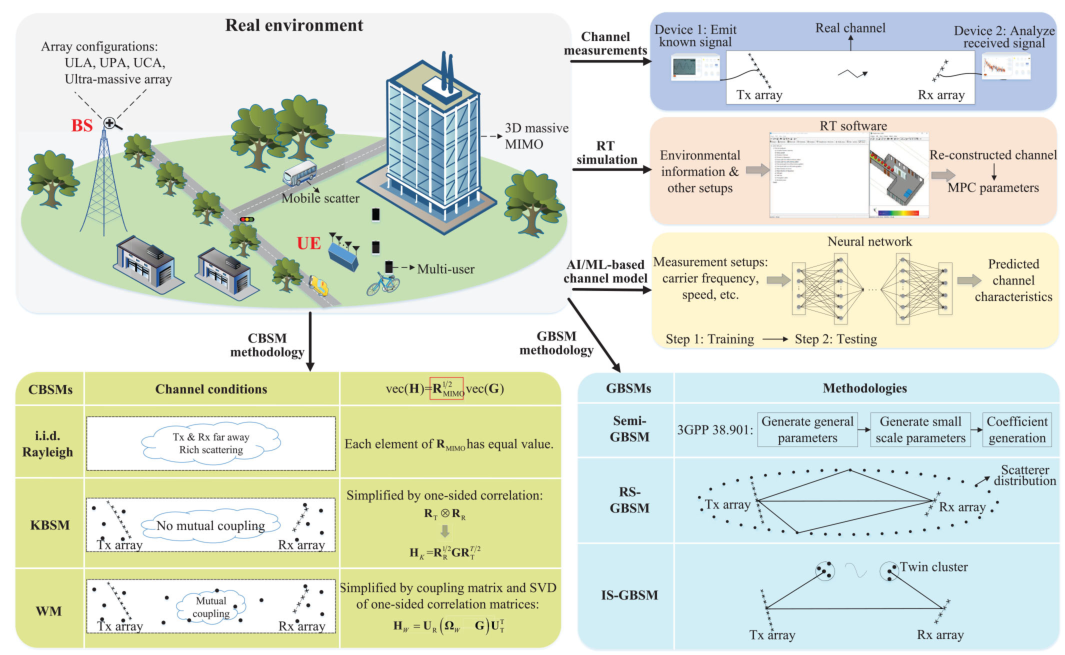
\includegraphics[width=\linewidth]{figures/Fig5.pdf}
%     \caption{Môi trường truyền thông MIMO kích thước lớn và một số mô hình kênh truyền tiêu biểu~\cite{Feng2022}.}
%     \label{fig:channel_model}
% \end{figure}

% Các mô hình kênh truyền MIMO kích thước lớn cũng đã được nhiều tác giả quan tâm nghiên cứu, tổng hợp và phân loại theo những hướng tiếp cận khác nhau như phân loại kênh truyền vật lý/toán học trong~\cite{Almers2007}, kênh xác định/ngẫu nhiên trong~\cite{Wang2018}, hay kênh tiên đoán/không tiên đoán trong~\cite{Feng2022}. Mô hình kênh vật lý biểu diễn kênh dưới dạng các thành phần đa đường trong đó mỗi thành phần được đặc trưng bởi các tham số như biên độ phức, độ trễ, góc đi, góc đến,~\ldots Trong khi đó, mô hình kênh toán học được thiết lập dưới dạng toán học có ma trận kênh với các phần tử là các biến ngẫu nhiên, phụ thuộc nhiều vào kênh và việc sắp đặt hệ thống như băng thông và cấu hình mảng ăng-ten. Mô hình kênh xác định/ngẫu nhiên phụ thuộc vào các tham số trong mô hình là các giá trị cố định hay các biến ngẫu nhiên. Mô hình kênh xác định thường đạt được từ việc giải phương trình Maxwell hay xấp xỉ phương trình truyền sóng trong khi mô hình kênh ngẫu nhiên mô tả các tham số kênh bằng phân bố xác suất. Phương pháp mô hình kênh xác định cho độ chính xác cao hơn nhưng cũng phải trả giá bằng độ phức tạp tính toán. Mô hình kênh tiên đoán dựa trên các thuật toán học máy với khả năng xử lý dữ liệu phi tuyến và tiên đoán để xác định các đặc trưng của kênh truyền. Hình~\ref{fig:channel_model} biểu diễn môi trường truyền thông của mMIMO và một số mô hình kênh truyền tiêu biểu. Nghiên cứu trong~\cite{Wang2018} chỉ ra rằng, vẫn còn sự chồng lấn, hạn chế trong các cách phân loại mô hình kênh truyền hiện nay. Trong luận văn, tác giả quan tâm đến một số mô hình kênh ngẫu nhiên cả vật lý và toán học, cụ thể là mô hình kênh ngẫu nhiên dựa trên tương quan (CBSM - Correlation-based Stochastic Model), mô hình kênh ngẫu nhiên dựa trên hình học (GBSM - Geometry-based Stochastic Model), và mô hình kênh ngẫu nhiên không dựa trên hình học (NGSM - Non Geometry-based Stochastic Model). Các mô hình này sẽ được tìm hiểu kỹ hơn ở những phần tiếp theo của luận văn. 

\subsection{Hệ thống truyền thông mMIMO}
\label{sec:mMIMO}

% \begin{figure}[htb]
%     \centering
%     \begin{tikzpicture}
%         \node[antenna, thick, scale=0.6] at (0, 0) (Tx0) {};
%         \node at (0, 17mm) (text_Tx0) {Tx $0$};
%         \draw[line] (-10mm, 0) -- (Tx0) node [pos=0, left] {$\mathbf{s}_0$};

%         \node[antenna, thick, scale=0.6] at (0, -25mm) (Tx1) {};
%         \node at (0, -8mm) (text_Tx1) {Tx $1$};
%         \draw[line] (-10mm, -25mm) -- (Tx1) node [pos=0, left] {$\mathbf{s}_1$};

%         \node[scale=1.5] at (0, -30mm) (dotss) {$\mathbf{\vdots}$};

%         \node[antenna, thick, scale=0.6] at (0, -55mm) (TxT) {};
%         \node at (0, -38mm) (text_TxT) {Tx $T-1$};
%         \draw[line] (-10mm, -55mm) -- (TxT) node [pos=0, left] {$\mathbf{s}_{T-1}$};

%         \node[antenna, thick, scale=0.6] at (70mm, 0) (Rx0) {};
%         \node at (70mm, 17mm) (text_Rx0) {Rx $0$};
%         \draw[line] (80mm, 0) -- (Rx0) node [pos=0, right] {$\mathbf{x}_{0}$};

%         \node[antenna, thick, scale=0.6] at (70mm, -25mm) (Rx1) {};
%         \node at (70mm, -8mm) (text_Rx1) {Rx $1$};
%         \draw[line] (80mm, -25mm) -- (Rx1) node [pos=0, right] {$\mathbf{x}_{1}$};

%         \node[scale=1.5] at (70mm, -30mm) (dotss) {$\mathbf{\vdots}$};

%         \node[antenna, thick, scale=0.6] at (70mm, -55mm) (RxL) {};
%         \node at (70mm, -38mm) (text_RxL) {Rx $L - 1$};
%         \draw[line] (80mm, -55mm) -- (RxL) node [pos=0, right] {$\mathbf{x}_{L-1}$};

%         \draw[arrow] (3mm, 6mm) -- (67mm, 6mm);
%         \draw[arrow] (3mm, 5mm) -- (67mm, -20mm);
%         \draw[arrow] (3mm, 4mm) -- (67mm, -49mm);

%         \draw[arrow] (3mm, -19mm) -- (67mm, 5mm);
%         \draw[arrow] (3mm, -20mm) -- (67mm, -21mm);
%         \draw[arrow] (3mm, -21mm) -- (67mm, -50mm);

%         \draw[arrow] (3mm, -49mm) -- (67mm, 4mm);
%         \draw[arrow] (3mm, -50mm) -- (67mm, -22mm);
%         \draw[arrow] (3mm, -51mm) -- (67mm, -51mm);

%         \node at (35mm, -60mm) (H) {$\mathbf{H} \in \mathbb{C}^{L \times T}$};
%     \end{tikzpicture}
%     \caption{Hệ thống truyền thông mMIMO.}
%     \label{fig:sys_model}
% \end{figure}

Xem xét một mô hình hệ thống thu phát mMIMO đơn giản với $T$ ăng-ten phát và $L$ ăng-ten thu. Hệ thống được biểu diễn dưới dạng toán học tại thời điểm $n$ như sau: 
\begin{equation}
\label{eq:timedomain}
    \mathbf{x}(n) = \mathbf{H}(n)*\mathbf{s}(n) + \mathbf{w}(n)
\end{equation}
trong đó $\mathbf{s}(n) \in \mathbb{C}^{T \times 1}$ là các ký hiệu được gửi đi từ $T$ bộ phát, ma trận $\mathbf{H} \in \mathbb{C}^{L\times T}$ biểu diễn kênh truyền, $\mathbf{x}(n) \in \mathbb{C}^{L \times 1}$ là véc-tơ biểu diễn tín hiệu thu được từ $L$ ăng-ten, và $\mathbf{w} \in \mathbb{C}^{L \times 1}$ là nhiễu cộng tính (AWGN).
Trong trường hợp kênh là pha-đinh phẳng tần số, còn được gọi là kênh băng hẹp thì phương trình~(\ref{eq:timedomain}) trở thành:  
\begin{equation}
    \mathbf{x}(n) = \mathbf{H}(n)\mathbf{s}(n) + \mathbf{w}(n)
\end{equation}
Các phần tử trong ma trận kênh được biểu diễn bởi các biến ngẫu nhiên phức có pha thường được mô hình bởi phân bố đều và phân bố biên độ tùy thuộc môi trường.


\subsection{Mô hình kênh CBSM}
Mô hình kênh CBSM thuộc loại mô hình kênh toán học, ngẫu nhiên.
Xét hệ mMIMO bất biến với thời gian có mô hình kênh hoàn chỉnh biểu diễn bởi phương trình~(\ref{eq:unstructure}).
\begin{equation}
    \label{eq:unstructure}
    \mathbf{H}_{total} = \beta \mathbf{H} 
\end{equation}
trong đó, $\beta$ đại diện cho ảnh hưởng của pha-đinh kích thước lớn gồm suy hao do khoảng cách truyền, pha-đinh bóng mờ, hiệu ứng chặn, và hấp thụ khí quyển; ma trận $\mathbf{H}$ đại diện cho ảnh hưởng của pha-đinh kích thước nhỏ, không có tia nhìn thẳng (NLOS). Xét ảnh hưởng của pha-đinh kích thước nhỏ, ma trận $\mathbf{H}$ được biểu diễn như sau:
\begin{equation}
    \mathbf{H} = \begin{bmatrix}
    h_{0,0} & \ldots  & h_{0, T-1} \\ 
    \vdots & \ddots & \vdots\\ 
    h_{L-1, 0} & \ldots  & h_{L-1, T-1}
    \end{bmatrix}
\end{equation}
với mỗi phần tử $h_{l,t}$ tương ứng là đáp ứng xung của kênh giữa ăng-ten phát thứ $t$ và ăng-ten nhận thứ $l$ (có thể dùng cho mô hình kênh băng rộng). 
Mô hình kênh được chia thành 2 loại: mô hình không tương quan và mô hình tương quan. Xét ma trận hiệp phương sai của ma trận kênh như sau:
\begin{equation}
    \label{eq:1.6}
    \mathbf{R}_{\mathbf{H}} = \mathbb{E} ({\operatorname{\mathbf{H}} \operatorname{\mathbf{H}}^H})
\end{equation}
với $(.)^H$ là phép biến đổi Hermitian.

Với mô hình kênh không tương quan, các phần tử của ma trận kênh được coi là có phân bố giống nhau và độc lập (i.i.d) hay hàm hiệp phương sai của ma trận kênh là một ma trận đường chéo với các giá trị đường chéo thường bằng 1. Với mô hình ma trận kênh i.i.d Rayleigh sẽ có các phần tử là các biến ngẫu nhiên Gauss phức trung bình bằng 0, phương sai bằng 1.


% \begin{equation}
%     \label{eq:correlation}
%     \operatorname{vec}(\mathbf{H}) = \mathbf{R}^{1/2}_{\mathbf{H}} \operatorname{vec} (\mathbf{G})
% \end{equation}
% trong đó, $\operatorname{vec}$ là phép véc-tơ hoá một ma trận, từ $\mathbf{H}$ kích thước $L\times T$ thành $LT \times 1$. Ký hiệu $\mathbf{G}$ biểu diễn ảnh hưởng của kênh khi không có sự tương quan giữa các phần tử như đã trình bày ở trên, $\operatorname{vec}(\mathbf{G})$ chứa các biến ngẫu nhiên i.i.d Gaussian có kỳ vọng bằng $0$ và phương sai $1$. Ma trận $\mathbf{R}_{\mathbf{H}}$ mô tả cấu trúc không gian của các mảng mMIMO, trong đó xem xét sự tương quan (correlation) lẫn nhau giữa các phần tử trong ma trận kênh truyền. Ma trận này được ước lượng như sau:
% Với mô hình kênh có sự tương quan, ma trận hiệp phương sai kênh~(\ref{eq:1.6}) có độ phức tạp tương ứng với $\mathcal{O}((LT)^2)$, tăng nhanh theo số phần tử ăng-ten trong hệ mMIMO. Phương pháp mô hình ngẫu nhiên Kronecker (KBSM - Kronecker-based Stochastic Model)~\cite{Chuah1998} được đề xuất để giảm thiểu độ phức tạp khi ước lượng $\mathbf{R}_{\mathbf{H}}$. 

% Trong đó, giả sử không có sự tương quan giữa mảng ăng-ten phát và thu, đồng thời không tồn tại các nguồn tán xạ giữa hai mảng ăng-ten này. Ma trận hiệp phương sai $\mathbf{R}_{\mathbf{H}}$ được phân tích thành:
% \begin{equation}
%     \mathbf{R}_{\mathbf{H}} = \mathbf{R}_{\text{tx}} \otimes \mathbf{R}_{\text{rx}}
% \end{equation}
% với $\mathbf{R}_{\text{tx}}$ và $\mathbf{R}_{\text{rx}}$ lần lượt là ma trận tương quan của các phần tử ăng-ten bên phát và thu, $\otimes$ là phép nhân Kronecker. Hai ma trận này lần lượt có dạng $\mathbf{R}_{\text{tx}} = \mathbb{E}(\mathbf{H}^\top \mathbf{H}^*)$ và $\mathbf{R}_{\text{rx}} = \mathbb{E}(\mathbf{H} \mathbf{H}^H)$, với $(.)^\top$ là phép chuyển vị ma trận. Dựa trên cấu trúc hình học của mảng ăng-ten, hai ma trận kể trên được xác định theo~\cite{Kshetrimayum2017}.


% \subsection{Mô hình kênh GBSM}
% \label{sec:GBSM}
% GBSM thuộc loại mô hình kênh vật lý có độ phức tạp cao. Mô hình này xem xét sự lan truyền của sóng vô tuyến trong không gian dưới dạng các cụm (cluster), tia/đường truyền riêng biệt. Việc xây dựng mô hình có thể dựa hoàn toàn trên dạng hình học của các phần tử tán xạ như mô hình RS-GBSM (Regular shaped - GBSM) có các tán xạ nằm trên các hình phổ biến như 1 vòng, 2 vòng, elíp,~\ldots, hay mô hình IS-GBSM (Irregular shaped - GBSM) với các tán xạ nằm trên các đường hình học không phổ biến như mô hình 2 cụm thể hiện đặc tính không dừng trong không gian của kênh mMIMO,~\ldots Ngoài ra, mô hình kênh Semi-GBSM cũng được sử dụng rất nhiều trong các chuẩn truyền thông di động. Ví dụ như: 3GPP phiên bản 16~\cite{r16} cho 5G hay WINNER II~\cite{WINNER}. So với GBSM, Semi-GBSM mặc dù có độ chính xác và khả năng mở rộng tốt hơn nhưng mô hình này lại có độ phức tạp lớn hơn nhiều do mô hình kênh không chỉ được xây dựng từ thông tin hình học của các cluster và phân bố của các tán xạ mà còn dựa trên môi trường được định nghĩa bởi người dùng, layout mạng và và thông số của mảng ăng-ten~\cite{Zhu2022}.
% %\begin{figure}[htb]
% %    \centering
% %    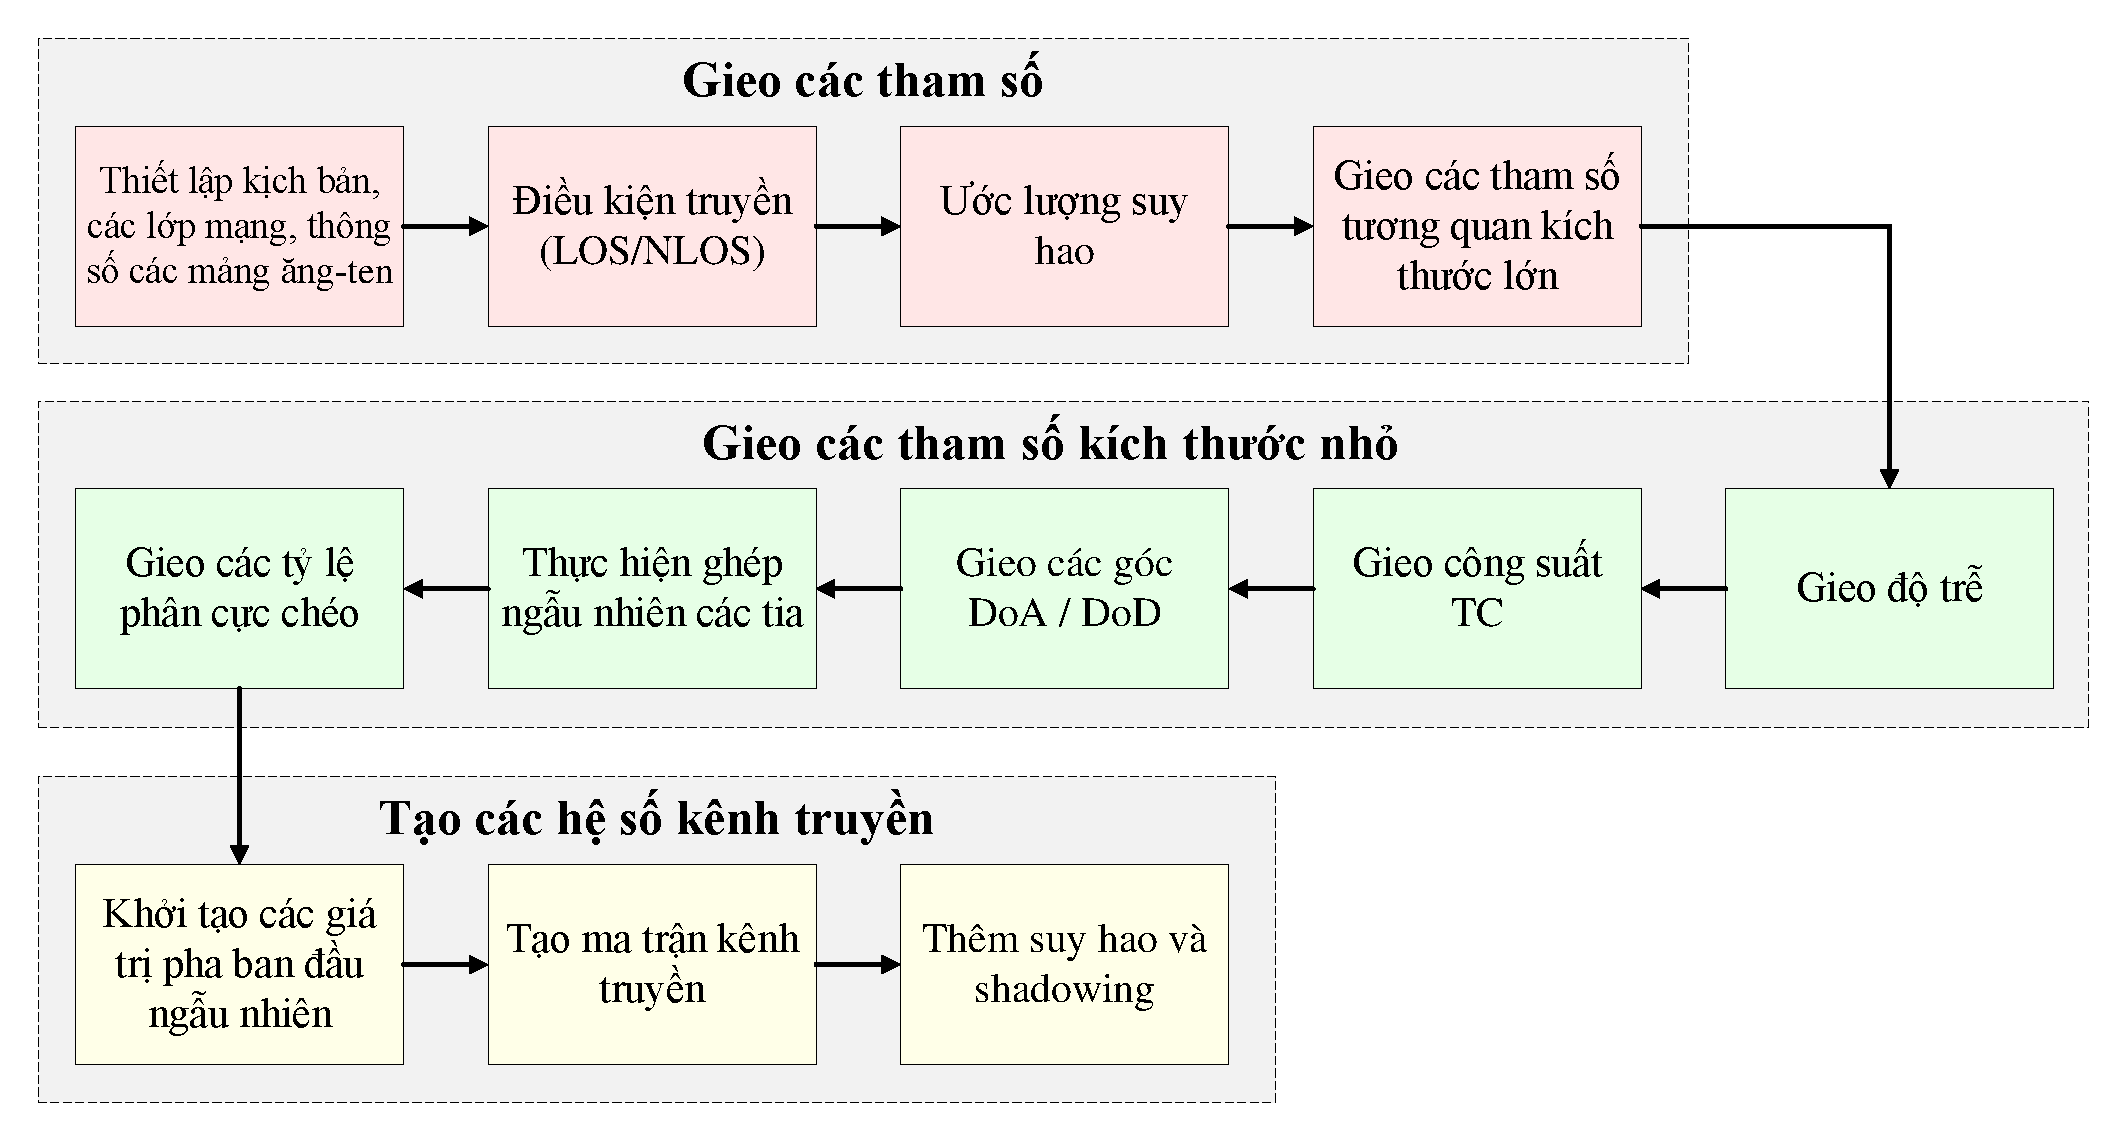
\includegraphics[width=\linewidth]{figures/3GPP_flow.pdf}
% %    \caption{Các bước tạo mô hình kênh truyền trong tiêu chuẩn 3GPP phiên bản 16~\cite{r16}.}
% %    \label{fig:3gpp_flow}
% %\end{figure}

% % Trên hình~\ref{fig:3gpp_flow} là 12 bước trong quá trình mô hình hoá kênh truyền mMIMO được đề ra trong tiêu chuẩn 3GPP phiên bản 16 dành cho các hệ thống 5G. Phần tiếp theo sẽ trình bày sơ lược về các nét chính trong phương pháp mô hình hoá này. 
% Theo mô hình GBSM, phần tử của ma trận kênh được tính bởi~\cite{Ju2021}:
% \begin{equation}
%     \label{eq:3gpp}
%     \begin{aligned}
%         {h}_{l, t}(n) = \sum\limits_{m=0}^{M-1} \sum\limits_{k=0}^{M_n - 1} \beta_{m, k, t} & \cdot e^{i\varphi_{m, k, t}} \cdot \delta\left(n-\tau_{m, k, t}\right) \\
%         &\cdot e^{-i k_s s_t(\theta^d_{m, k, t}, \phi^d_{m, k, t})} \cdot
%         e^{-i k_s s_l(\theta^a_{m, k, t}, \phi^a_{m, k, t})} 
%     \end{aligned}
% \end{equation}
% $M, M_n$ lần lượt là số lượng các cụm và số lượng các tia trong mỗi cụm đến bên thu. Với tia thứ $k$ trong cụm thứ $m$, các ký hiệu $\beta, \varphi, \tau$ đại diện cho biên độ, pha, và thời gian trễ tuyệt đối của mỗi tia. Góc ngẩng (zenith), góc phương vị (azimuth) của hướng sóng đi (DoD - Direction of Departure) và hướng sóng đến (DoA - Direction of Arrival) được ký hiệu lần lượt là $\theta^d, \phi^d, \theta^a$, và $\phi^a$. Ký hiệu $(\cdot)$ tương ứng là phép nhân vô hướng. Các thành phần biên độ $\beta_{m,k,t}$ của $h_{l, t}$ phụ thuộc vào suy hao, như một hàm của tần số sóng mang $f_c$, khoảng cách giữa ăng-ten phát và ăng-ten thu $d$, cho bởi:
% \begin{equation}
%     \label{eq:FSPL}
%     \begin{aligned}
%         \beta_{m, k, t}(f_c, d)[\mathrm{dB}]=& \mathrm{FSPL}\left(f_c, d_{0}\right)+10 \xi \log _{10}\left(\frac{d}{d_{0}}\right)+\chi_{\sigma}, \\
%         & \text { với } d \geq d_{0}, \text { khi } d_{0}=1\mathrm{m}
%     \end{aligned}
% \end{equation}
% trong đó, $\operatorname{FSPL}\left(f_c, d_{0}\right)=20 \log _{10}\left(4 \pi d_{0} c / f_c\right)$, $c$ là vận tốc ánh sáng, $\xi$ đại diện cho hệ số mất mát hàm mũ (PLE - Path Loss Exponent), và $\chi_{\sigma}$ là đại diện cho hiệu ứng pha-đinh bóng mờ và được mô hình hoá dưới dạng một biến ngẫu nhiên lognormal trung bình bằng 0 và độ lệch chuẩn $\sigma$. 
% Các thông số trong các phương trình (\ref{eq:3gpp}) và (\ref{eq:FSPL}) được quy định và đo đạc xác định cho từng môi trường khác nhau. Đặc trưng của kĩ thuật semi-GBSM là ngoài sử dụng các tham số ngẫu nhiên, rất nhiều tham số của kênh truyền đã được đo lường từ trước và cố định với mỗi điều kiện cụ thể.
% Ví dụ, việc xác định số lượng các TC, trên bảng~\ref{tab:num_TC} chỉ ra các thông số được đo đạc này cho bốn loại môi trường cụ thể, bao gồm: UMi - khu dân cư kích cỡ micro, UMa - khu dân cư kích cỡ macro, RMa - khu nông thông kích cỡ macro, và điều kiện văn phòng trong nhà. Mỗi môi trường trên, các kịch bản đo được thiết lập ở 2 hoặc 3 tình huống gồm: tầm nhìn thẳng (LOS - Line of Sight), không tầm nhìn thẳng (NLOS - Non-LOS), và từ bên ngoài vào trong nhà (O2I - Outdoor to Indoor).
% \begin{table}
% \centering
% \caption{Số lượng các TC và sub-path trong mỗi TC theo chuẩn 3GPP phiên bản 16~\cite{r16}.}
% \label{tab:num_TC}
% \begin{tabular}{|l|c|c|c|c|c|c|} 
% \hline
% \multicolumn{1}{|c|}{\multirow{2}{*}{\textbf{Thông số}}} & \multicolumn{3}{c|}{\begin{tabular}[c]{@{}c@{}}\textbf{UMi - Khu dân cư,}\\\textbf{kích cỡ micro}\end{tabular}} & \multicolumn{3}{c|}{\begin{tabular}[c]{@{}c@{}}\textbf{UMa - Khu dân cư,}\\\textbf{~kích cỡ macro~}\end{tabular}} \\ 
% \cline{2-7}
% \multicolumn{1}{|c|}{} & \textbf{LOS} & \textbf{NLOS} & \textbf{O2I} & \textbf{LOS} & \textbf{NLOS} & \textbf{O2I} \\ 
% \hline
% \textbf{Số lượng TC} & 12 & 19 & 12 & 12 & 20 & 12 \\ 
% \hline
% \textbf{Số lượng sub-path mỗi TC} & 20 & 20 & 20 & 20 & 20 & 20 \\ 
% \hline
% \multicolumn{1}{|c|}{\multirow{2}{*}{\textbf{Thông số}}} & \multicolumn{3}{c|}{\begin{tabular}[c]{@{}c@{}}\textbf{\textbf{RMa - Khu nông thôn,}}\\\textbf{\textbf{~kích cỡ macro~}}\end{tabular}} & \multicolumn{3}{c|}{\begin{tabular}[c]{@{}c@{}}\textbf{\textbf{Văn phòng,}}\\\textbf{\textbf{~trong nhà}}\end{tabular}} \\ 
% \cline{2-7}
%  & \textbf{LOS} & \textbf{NLOS} & \textbf{O2I} & \textbf{LOS} & \multicolumn{2}{c|}{\textbf{NLOS}} \\ 
% \hline
% \textbf{Số lượng TC} & 11 & 10 & 10 & 15 & \multicolumn{2}{c|}{19} \\ 
% \hline
% \textbf{Số lượng sub-path mỗi TC} & 20 & 20 & 20 & 20 & \multicolumn{2}{c|}{20} \\
% \hline
% \end{tabular}
% \end{table}

% Tiếp đến, độ dịch pha ban đầu của các sub-path trong mỗi TC cũng được 3GPP đưa ra như trên bảng~7.5-3 tại tài liệu~\cite{r16}.
% \begin{table}
% \centering
% \caption{Độ lệch pha của các sub-path trong một TC.}
% \label{tab:phase}
% \begin{tabular}{|c|c|c|c|} 
% \hline
% \multicolumn{1}{|c|}{\textbf{sub-path \#}} & \multicolumn{1}{c|}{$\varphi_{n,m,t} (^\circ)$} & \textbf{\textbf{sub-path \#}} & $\varphi_{n,m,t} (^\circ)$ \\ 
% \hline
% 1, 2 & $\pm$ 0,0447 & 11, 12 & $\pm$0,6797 \\ 
% \hline
% 3, 4 & $\pm$ 0,1413 & 13, 14 & $\pm$0,8844 \\ 
% \hline
% 5, 6 & $\pm$ 0,2492 & 15, 16 & $\pm$1,1481 \\ 
% \hline
% 7, 8 & $\pm$ 0,3715 & 17, 18 & $\pm$1,5195 \\ 
% \hline
% 9, 10 & $\pm$ 0,5129 & 19, 20 & $\pm$2,1551 \\
% \hline
% \end{tabular}
% \end{table}
% Thông tin về tỷ lệ công suất của các sub-path trong mỗi TC và độ trễ của chúng so với sub-path đến sớm nhất được trình bày trên bảng~7.5-5 tại tài liệu~\cite{r16}. Cụ thể, mỗi TC sẽ được chia nhỏ hơn nữa thành 3 cụm con (SC - Sub-cluster). Các sub-path sẽ được chia vào một trong ba SC trên dựa trên thời gian trễ của chúng so với tia đến sớm nhất. Bốn thông số còn lại bao gồm $\theta$ và $\phi$ của bên thu và phát được biểu diễn dưới dạng các giá trị ngẫu nhiên thuộc các phân bố khác nhau tuỳ thuộc vào điều kiện môi trường truyền thông, chi tiết xem trong các bảng từ 7.5-6 đến 7.5-10 tại~\cite{r16}.
% \begin{table}
% \centering
% \caption{Thông tin về công suất và độ trễ của các sub-path trong mỗi TC.}
% \label{tab:SC}
% \begin{tabular}{|c|c|c|c|} 
% \hline
% \vcell{\textbf{SC \#}} & \vcell{\textbf{sub-path \#}} & \vcell{\begin{tabular}[b]{@{}c@{}}\textbf{Tỷ lệ công suất}\\\textbf{($\beta_{n, m, t} / \sum_{m=1}^{M} \beta_{n, m, t}$)}\end{tabular}} & \vcell{\begin{tabular}[b]{@{}c@{}}\textbf{Trễ tuyệt đối}\\\textbf{($\tau_{n, m, t} - \tau_{n, 1, t}$)}\end{tabular}} \\[-\rowheight]
% \printcelltop & \printcelltop & \printcelltop & \printcelltop \\ 
% \hline
% 1 & 1, 2, 3, 4, 5, 6, 7, 8, 19, 20 & 10/20 & 0 ns \\ 
% \hline
% 2 & 9, 10, 11, 12, 17, 18 & 6/20 & 5 ns \\ 
% \hline
% 3 & 13, 14, 15, 16 & 4/20 & 10 ns \\
% \hline
% \end{tabular}
% \end{table}


\subsection{Mô hình kênh NGSM}
\label{sec:NGSM}
NGSM là mô hình kênh ngẫu nhiên vật lý không dựa trên phân bố hình học của các nguồn tán xạ, điển hình là mô hình kênh SV (Saleh Valenzuela).
Mô hình kênh SV được đề xuất với độ phức tạp nhỏ hơn nhiều so với mô hình GBSM. 
% Do vậy, mô hình kênh NGSM hiện nay được xem xét dưới dạng là các mô hình tham số (parametric)~\cite{Le2018, Swindlehurst2022}. Mô hình này vẫn kế thừa đặc trưng không gian của GBSM khi xem xét việc truyền sóng theo các đường khác nhau trong không gian 3D (DoA, DoD và cấu trúc mảng ăng-ten được gộp trong $\varphi$).
Cụ thể là: thay vì chia thành các cụm, các tia với các góc, độ trễ khác nhau, mô hình SV gộp các cụm thành các đường truyền lớn với điều kiện xem xét đặc trưng là tính thưa trong các hệ truyền thông sử dụng sóng mi-li-mét. Các thành phần suy hao, dịch pha, và độ trễ được gộp chung lại thành một hệ số khuếch đại phức ($\beta$). Khi đó các phần tử của ma trận kênh được biểu diễn dưới dạng:
\begin{equation}
    h_{l, t} = \sum\limits_{m=0}^{M-1} \beta_{m, t} \cdot e^{\varphi_{l, m, t}} 
\end{equation}
với $\beta$ và $\varphi_l(\theta, \phi)$  là các biến ngẫu nhiên.
Trong chương~\ref{sec:CRB} của luận văn, mô hình kênh truyền này được gọi là ``\textbf{có cấu trúc}'' (structured) để phân biệt với không sử dụng cấu trúc trong CBSM.


\subsection{Đánh giá các phương pháp mô hình kênh cho mMIMO}

Theo đánh giá trong các công bố trước đó đã chỉ ra: kênh xác định cho độ chính xác cao nhưng độ phức tạp tính toán cũng cao và tính tổng quát thấp; kênh CBSM cho cả ba thông số đều thấp nhưng lại rất thuận tiện trong phân tích; và cuối cùng là kênh GBSM cho độ chính xác vừa đủ, độ phức tạp trung bình và tính tổng quát cao.
% chính xác thấp cho tốc độ bít lớn nhất tương đương với mô hình kênh truyền xác định qua đo đạc, do đây cũng là hai phương pháp gần nhất với môi trường truyền thông không dây thực tế. Điểm hạn chế của cả hai phương pháp xác định và GBSM nằm ở độ phức tạp trong các bài toán nghiên cứu. Với trường hợp mô hình kênh như của 3GPP đã được trình bày ở trên, phải cần đến 12 bước theo như tài liệu gốc tại~\cite{r16} để mô hình hoá một kênh truyền cho một điều kiện truyền thông cụ thể duy nhất. Do vậy, hai phương pháp này cũng khó có tính tổng quát trong các bài toán nghiên cứu khi cố gắng tìm các giải thuật ước lượng kênh truyền phục vụ nhiều loại môi trường truyền nhất có thể.
% Với phương pháp RT, công việc khó nhất đó là xây dựng mô hình 3D của môi trường truyền, không thể mô phỏng chính xác tuyệt đối, yêu cầu môi trường truyền bất biến trong quá trình mô phỏng, và yêu cầu tài nguyên tính toán khổng lồ nên khó để đưa vào các hệ thống thời gian thực. 

Từ những phân tích trên, luận văn lựa chọn hai mô hình kênh đơn giản với mục đích giảm độ phức tạp tính toán trong các nghiên cứu tại các chương sau. Hai mô hình kênh truyền ngẫu nhiên này là \textbf{i.i.d Rayleigh (không sử dụng cấu trúc)} và \textbf{NGSM (có cấu trúc)} được sử dụng phù hợp với các nghiên cứu lý thuyết về ước lượng kênh truyền tiếp theo.

\section{Các phương pháp nhận dạng hệ thống MIMO kích thước lớn}

Ngày nay, các thuật toán ước lượng kênh truyền không dây đã đạt được các bước tiến đáng kể về độ chính xác. Dựa trên đặc điểm của các thuật toán có thể chia thành bốn hướng như trên hình~\ref{fig:classify}, bao gồm: phương pháp không mù (NB), mù (B), bán mù (SB), và dựa trên học máy, học sâu (AI-based). 
% Với mỗi phương pháp, rất nhiều thuật toán đã được đề xuất và cho hiệu quả tốt trong các tình huống cụ thể. Phần này sẽ thực hiện việc tìm hiểu về một số thuật toán nhận dạng kênh tiêu biểu, bao gồm:  như các trích dẫn trên hình~\ref{fig:classify}.
% Từ cách phân loại kể trên, đôi nét cơ bản về các phương pháp ước lượng kênh truyền này sẽ được trình bày, trong đó, một số thuật toán được dùng để so sánh kết quả trong các chương sau của luận văn sẽ được trình bày chi tiết.

\begin{figure}[ht]
    \centering
    \begin{tikzpicture}
        \node (b1) [startstop] at (0, 0) {Các phương pháp nhận dạng kênh truyền không dây};

        \node (b21) [process, align=center] at (-60mm, -25mm) {Phương pháp không mù};

        \node (b22) [process, align=center] at (-20mm, -25mm) {Phương pháp mù};

        \node (b23) [process, align=center] at (20mm, -25mm) {Phương pháp bán mù};

        \node (b24) [process, align=center] at (60mm, -25mm) {Học máy/Học sâu};

        \node (b31) [below=8mm of b21, process, align=left, fill=green!10!white] {
        - Sử dụng dữ liệu \\
        % \hspace{0.1cm} + Dựa trên đào tạo~\cite{Singh2019} \\
        \hspace{0.1cm} + Dựa trên Pilot \\
        \hspace{0.3cm} * ZF~\cite{Yang2015} \\
        \hspace{0.3cm} * MMSE~\cite{Jiang2011} \\
        \hspace{0.3cm} * Maximum \\ 
        \hspace{0.3cm} Likelihood~\cite{ljung1999system} \\
        - Hướng quyết định~\cite{Ozdemir2007} \\
        \hspace{0.1cm} + Quyết định cứng \\
        \hspace{0.1cm} + Quyết định mềm 
        };

        \node (b32) [below=8mm of b22, process, align=left, fill=green!10!white] {
            - Xác định \\
            \hspace{0.3cm} * FA~\cite{HAJJI2018} \\
            - Tính thống kê \\
            \hspace{0.1cm} + Bậc hai~\cite{Tong1994} \\
            \hspace{0.3cm} * MRE~\cite{original} \\
            \hspace{0.1cm} + Bậc cao~\cite{abed1997}\\
            \hspace{0.3cm} * CMA~\cite{Treichler1983} \\
        };

        \node (b33) [below=8mm of b23, process, align=left, fill=green!10!white] {
            - {\color{red} Sử dụng một phần} \\
            {\color{red}dữ liệu}~\cite{Rekik2021, Ladaycia2017, Ladaycia2019} \\
            - {\color{red} Sử dụng DoA/} \\
            {\color{red}DoD}~\cite{Wang2016} \\
            - Sử dụng vị trí~\cite{Lin2020}
        };

        \node (b34) [below=8mm of b24, process, align=left, fill=green!10!white] {
            - Học cổ điển \\
            \hspace{0.3cm} * Hồi quy~\cite{Simeon2022} \\
            - Mạng nơ-ron \\
            \hspace{0.3cm} * {\color{red} DetNet}~\cite{Samuel2019} \\
            - Học tăng cường \\
            \hspace{0.3cm} * Q-learning~\cite{Oh2021}
        };

        \draw[line] (b1.south) -- ([yshift=-5mm]b1.south);
        \draw[arrow] ([yshift=-5mm]b1.south) -| (b21);
        \draw[arrow] ([yshift=-5mm]b1.south) -| (b22);
        \draw[arrow] ([yshift=-5mm]b1.south) -| (b23.north);
        \draw[arrow] ([yshift=-5mm]b1.south) -| (b24.north);

        \draw[arrow] (b21) -- (b31);
        \draw[arrow] (b22) -- (b32);
        \draw[arrow] (b23) -- (b33);
        \draw[arrow] (b24) -- (b34);
        
    \end{tikzpicture}
    \caption{Phân loại các phương pháp ước lượng kênh truyền viễn thông.}
    \label{fig:classify}
\end{figure}

\subsection{Nhận dạng kênh không mù}
Như trên hình~\ref{fig:classify}, các phương pháp nhận dạng kênh không mù có thể chia làm hai nhóm chính, bao gồm các phương pháp sử dụng pilot (Pilot-assisted) và các phương pháp dựa trên hướng quyết định (Decision-directed). 
% Các thuật toán sử dụng dữ liệu có thể chia làm hai loại nhỏ hơn, gồm có các phương pháp dựa trên việc huấn luyện (Training-based) và các phương pháp dựa trên tín hiệu hoa tiêu (Pilot-assisted). Khác biệt chính giữa hai phương pháp là loại tín hiệu được dùng để ước lượng kênh truyền. Với Training-based, bên phát sẽ gửi các dữ liệu huấn luyện gốc, bên thu chỉ biết thời điểm dữ liệu huấn luyện này được truyền nhưng không biết trước thông tin của dữ liệu. Tín hiệu bên thu nhận được gồm tín hiệu gốc và tín hiệu đã bị méo khi đi qua kênh truyền. Mô hình ước lượng được huấn luyện bằng cách tối ưu hóa hàm mất mát giữa kết quả ước lượng kênh truyền và giá trị thực tế của kênh truyền.
Với Pilot-assisted, các ký hiệu pilot được chèn trực tiếp vào khung dữ liệu gửi đi, bên thu biết cả thời gian, vị trí, và giá trị gốc của các ký hiệu pilot này. Từ đó, bên thu có thể ước lượng ra ảnh hưởng của kênh truyền đến các tín hiệu pilot và nội suy ra ảnh hưởng của kênh truyền đến toàn bộ dữ liệu còn lại. Các giải thuật phổ biến được sử dụng cho phương pháp Pilot-assisted có thể kể đến như bộ phát hiện ép không (ZF - Zero Forcing), lỗi bình phương trung bình tối thiểu (MMSE - Minimum Mean Square Error). 
% Hai giải thuật này là giải thuật tuyến tính và được trình bày chi tiết ở phía dưới.
% , lần lượt ở mục~\ref{sec:zf} và~\ref{sec:mmse}. 
Tuy phổ biến và được áp dụng trong các hệ truyền thông thực tế, nhưng các phương pháp sử dụng dữ liệu để ước lượng kênh truyền có một nhược điểm đó là giảm hiệu quả sử dụng phổ do một phần băng thông bị lãng phí để truyền tải các dữ liệu huấn luyện (pilot).

% \subsubsection*{\textbf{Bộ nhận dạng ZF}} \label{sec:zf}

% Thuật toán nhận dạng tuyến tính thường dựa trên các phép biến đổi tuyến tính các tín hiệu nhận được $\mathbf{x}$. Các giải thuật này thường có độ phức tạp thấp hoặc trung bình. Tuy nhiên, độ phức tạp sẽ tăng lên nếu hệ thống có số chiều lớn, ví dụ số lượng ăng-ten $T$ hay $L$ rất lớn trong mMIMO dẫn đến phép nghịch đảo ma trận tiêu tốn nhiều tài nguyên tính toán hơn. Một bộ nhận dạng tuyến tính có thể biểu diễn bởi:
% \begin{equation}
%     \mathbf{s} = \mathbf{G} \mathbf{x}
% \end{equation}

% ZF là thuật toán đơn giản nhất trong các bộ nhận dạng tuyến tính. Trong đó, ma trận kênh truyền $\mathbf{H}$ sẽ được nghịch đảo để loại bỏ ảnh hưởng của kênh truyền. Ma trận làm bằng $\mathbf{G}_{ZF}$ của bộ nhận dạng ZF như sau:
% \begin{equation}
%     \mathbf{G}_{ZF}=\left(\mathbf{H}^H \mathbf{H}\right)^{-1} \mathbf{H}^H
% \end{equation}
% Với $\mathbf{G}_{ZF}$, tín hiệu gốc được khôi phục/ước lượng bởi công thức:
% \begin{equation}
%     \hat{\mathbf{s}}_{ZF}=\left(\mathbf{H}^H \mathbf{H}\right)^{-1} \mathbf{H}^H \mathbf{x}
% \end{equation}

% \subsubsection*{\textbf{Bộ nhận dạng MMSE}} \label{sec:mmse}

% Hiệu năng của bộ nhận dạng ZF thường bị ảnh hưởng bởi tạp âm AWGN. Do vậy, bộ nhận dạng MMSE kết hợp thêm thông tin phương sai của nhiễu trước khi nghịch đảo ma trận để đạt được độ chính xác cao hơn. Ma trận làm bằng $\mathbf{G}_{MMSE}$ của bộ nhận dạng MMSE được biểu diễn dưới dạng:
% \begin{equation}
%     \mathbf{G}_{MMSE}=\left(\mathbf{H}^H \mathbf{H}+\frac{\sigma^2}{\mathbb{E}(\mathbf{s})} \mathbf{I}\right)^{-1} \mathbf{H}^H
% \end{equation}
% với $\sigma^2$ là phương sai của nhiễu AWGN, $\mathbb{E}(\mathbf{s})$ là công suất trung bình của mỗi ký hiệu gửi đi, và $\mathbf{I}$ là ma trận đơn vị. Với $\mathbf{G}_{MMSE}$, tín hiệu gốc được khôi phục như sau:
% \begin{equation}
%     \hat{\mathbf{s}}_{MMSE}=\left(\mathbf{H}^H \mathbf{H}+\frac{\sigma^2}{\mathbb{E}(\mathbf{s})} \mathbf{I}\right)^{-1} \mathbf{H}^H \mathbf{x}
% \end{equation}

% % Ưu điểm của MMSE, các giá trị thấp trong quá trình nghịch đảo có thể dẫn đến hiện tượng khuếch đại tạp âm (deep null) khi sử dụng ZF, được khắc phục bởi công suất tạp âm khác không. Tuy nhiên,
% Có thể nhận thấy cả hai bộ nhận dạng ZF và MMSE đều cần các chuỗi pilot để ước lượng kênh truyền trước khi ước lượng tín hiệu gốc.
% , sau đó nội suy ra ma trận $\mathbf{H}$.
% \subsection{Maximum Likelihood Detector (MLD)}

\subsection{Nhận dạng kênh mù} \label{sec:blind}

Các thuật toán nhận dạng ``mù'' (B - Blind) ở đây được hiểu là khi xử lý (nhận dạng), bộ xử lý ``không nhìn thấy'' (không có thông tin) của đầu vào. Các thuật toán xử lý tín hiệu mù phát triển mạnh trong thập kỷ 90, tuy nhiên các phương pháp xử lý mù thường yêu cầu các thông số thống kê của tín hiệu mà thông thường không biết trước trong các hệ thống truyền thông thực, hơn nữa, độ chính xác mà các thuật toán này đưa ra cũng thấp hơn đáng kể khi so sánh với các phương pháp sử dụng pilot truyền thống. Do vậy, các thuật toán mù cũng ít được quan tâm trong những thế hệ mạng viễn thông di động trước 5G.

\subsection{Nhận dạng kênh bán mù} \label{sec:semi}

Các thuật toán nhận dạng ``bán mù'' (SB - Semi-Blind) là phương pháp cải tiến của B và được quan tâm trong các năm gần đây. Đây là kỹ thuật kết hợp các thông tin từ hướng tiếp cận mù truyền thống 
và các dạng thông tin khác, ví dụ: hướng sóng đến (DoA - Direction of Arrival), toạ độ người dùng,~\ldots. Điều này giúp tăng độ chính xác, giảm độ phức tạp, và cho khả năng ứng dụng rộng rãi hơn. Trong một số trường hợp, hiệu quả của từ các dạng thông tin khác này có thể giúp giảm đi số lượng pilot cần thiết cho việc nhận dạng hệ thống nhằm tăng hiệu suất phổ nhưng vẫn giữ được độ chính xác cần thiết.

Các phương pháp nhận dạng hệ thống sử dụng các thông tin khác với thông tin từ các ký hiệu pilot như trong hướng tiếp cận bán mù kể trên được gọi là tri thức mới.

\subsection{Nhận dạng kênh sử dụng học máy}

Các thuật toán nhận dạng sử dụng học máy, học sâu (ML - Machine Learning; DL - Deep Learning) cũng là lĩnh vực nghiên cứu dành được nhiều sự quan tâm trong các năm gần đây. Ưu điểm của các kỹ thuật sử dụng ML/DL là tính đa dạng, khi hướng tiếp cận ML/DL sử dụng cho mục đích xử lý các loại tín hiệu như hình ảnh, âm thanh đã đạt được các bước tiến rõ rệt. Đầu vào của các mạng DL được sử dụng để nhận dạng hệ thống rất linh hoạt, có thể tương ứng với cả ba hướng tiếp cận: pilot, mù, và bán mù kể trên. Sau quá trình huấn luyện, các mô hình (model) học máy có thể hoạt động độc lập như một bộ cân bằng mù/bán mù, khi chỉ cần đưa các tín hiệu thu được đi qua mô hình, và các tín hiệu cần khôi phục sẽ được trả về mà không cần đến các chuỗi pilot, hay thông tin về trạng thái kênh truyền (CSI - Channel State Information).

\newpage
\clearpage
\phantomsection

\setcounter{chapter}{1}
\chapter[{ĐÁNH GIÁ ẢNH HƯỞNG CỦA CẤU HÌNH MẢNG ĂNG-TEN TRONG NHẬN DẠNG HỆ THỐNG MIMO KÍCH THƯỚC LỚN}]{Đánh giá ảnh hưởng của cấu hình mảng ăng-ten trong nhận dạng hệ thống MIMO kích thước lớn}
\label{sec:CRB}

\section{Mô hình kênh truyền có cấu trúc với các cấu hình mảng ăng-ten khác nhau}\label{SM}

Mô hình toán học của một hệ thống mMIMO sử dụng điều chế ghép kênh phân chia theo tần số trực giao với $K$ sóng mang con trong kênh đường lên gồm $T$ ăng-ten phát và $L$ ăng-ten thu. Mỗi ký hiệu OFDM bao gồm $K$ ký hiệu dữ liệu và một phần tiền tố vòng. Tại ăng-ten thu thứ $l$, sau khi đã loại bỏ thành phần CP và thực hiện biến đổi Fourier, tín hiệu đầu ra tại ăng-ten thu thứ $l$ như sau:
\begin{equation}
    \mathbf{x}_{l}=\sum_{t=0}^{T-1} \mathcal{F} \mathcal{T}\left(h_{l, t}\right) \frac{\mathcal{F}}{K} \mathbf{s}_{j}+\mathbf{w}_{l}
\end{equation}
trong đó $\mathcal{F}$ đại diện cho ma trận Fourier rời rạc, gồm $K$ điểm và $\mathcal{T}$ là ma trận lặp lại của $h_{l, t}$. Tiếp đến, $\mathbf{s}_{j}$ là ký hiệu OFDM thứ $k$ có độ dài $K$ và $\mathbf{w}_{l} \in \mathbb{C}^{K \times 1}$ là tạp âm AWGN có dạng i.i.d phân bố Gauss $\mathcal{C} \mathcal{N}\left({0}, \sigma_{\mathbf{w}}^{2} \mathbf{I}_L\right)$. 
Cuối cùng, $h_{l, t}$ là hệ số kênh thuộc ma trận kênh truyền được biểu diễn dưới dạng véc-tơ $\mathbf{h} \in \mathbb{C}^{L T \times 1}$.
Giả sử rằng $M$ là số lượng đường truyền giữa một cặp ăng-ten phát, thu. Dựa trên hướng tiếp cận mô hình kênh truyền có cấu trúc, $h_{l, t}$ được mô hình tương ứng với $M$ đường truyền như sau:
\begin{equation}
\label{eq:2}
    % \begin{aligned}
        h_{l, t} = \sum\limits_{m=0}^{M-1} \beta_{m, t} e^{\varphi_{m, t}} = \sum\limits_{m=0}^{M-1} \beta_{m, t} \cdot e^{-i k_s c_l(\theta_{m, t}, \phi_{m, t})} 
    % \end{aligned}
\end{equation}
tại tia thứ $m$, hệ số $\beta$ biểu diễn cho hệ số khuếch đại phức. Góc ngẩng và góc phương vị của hướng sóng đến (DoA)\footnote{Để đơn giản hoá, thông tin về DoD được coi là không biết trước tại bên thu của kênh đường lên.} lần lượt là  $\theta$, $\phi$. Các ký hiệu còn lại lần lượt là:
\begin{equation}
    \begin{aligned}
        &k_s = 2\pi/\lambda \\
        &c_l(\theta_{m, t}, \phi_{m, t}) = \widehat{\boldsymbol{c}} \cdot \boldsymbol{c}_l \\
        &\widehat{\boldsymbol{c}}=\sin \theta_{m, t} \cos \phi_{m, t} \widehat{\boldsymbol{x}}+\sin \theta_{m, t} \sin \phi_{m, t} \widehat{\boldsymbol{y}}+\cos \theta_{m, t} \widehat{\boldsymbol{z}} \\
        &\boldsymbol{c}_l=x_{l} \widehat{\boldsymbol{x}}+y_{l} \widehat{\boldsymbol{y}}+z_{l} \hat{\boldsymbol{z}}
    \end{aligned}
\end{equation}
trong đó, $\lambda$ là bước sóng; $\widehat{\boldsymbol{c}}$ là véc-tơ đơn vị trong hệ toạ độ đề-các (Descartes) ba chiều của DoA; và $\boldsymbol{c}_l$ là vị trí của phần tử thứ $l$ trong mảng ăng-ten bên thu ứng với toạ độ ($x_l, y_l, z_l$).

Hai cấu hình của các mảng ăng-ten mảng thẳng các đều (ULA) và cấu hình mảng trụ cách đều (UCyA), được khảo sát trong luận văn. Ứng với mảng 1D, ULA là mảng ăng-ten thẳng đơn giản nhất có $N_{ULA}$ phần tử cách đều nhau một khoảng $d_{2D}$. Ứng với mảng ăng-ten 3D, cấu hình UCyA gồm $N_{3D}$ lớp của $N_{UCA}$ phần tử thuộc một mảng tròn cách đều (UCA - Uniform Circle Array) được xem xét. Với khoảng cách giữa các phần tử trong mảng UCA cũng là $d_{2D}$ và khoảng cách giữa các lớp của UCyA là $d_{3D}$ theo hướng dọc trục $z$. 
% Từ đó, bán kính $r$ của mảng vòng UCA được tính như sau:
% \begin{equation}
%     r = \frac{1/2 \cdot d_{2D}}{\sin(\pi/N_{UCA})}
% \end{equation}

% Toạ độ ($\boldsymbol{c}_l$) của các phần tử trong hai cấu hình mảng ăng-ten nêu trên là:
% \begin{align} 
%     &\boldsymbol{c}_l(\text{ULA}) = \;\; \begin{cases}
%     x_l = n_{ULA} * d_{2D}\\ 
%     y_l = 0\\ 
%     z_l = 0
%     \end{cases}
%     \\
%     &\boldsymbol{c}_l(\text{UCyA}) = \begin{cases}
%     x_l = r * \sin(n_{UCA} * \frac{2\pi}{N_{UCA}})\\ 
%     y_l = r * \cos(n_{UCA} * \frac{2\pi}{N_{UCA}})\\ 
%     z_l = n_{3D} * d_{3D}
%     \end{cases}
% \end{align}
% với $n_{ULA} = 0, 1, \ldots, N_{ULA}-1$; $n_{UCA} = 0, 1, \ldots, N_{UCA}-1$, và $n_{3D} = 0, 1, \ldots, N_{3D}-1$.


\section{Đường bao Cramér Rao cho giải thuật nhận dạng hệ thống không mù và bán mù}\label{CRB}

% Trong mục này, tác giả sẽ trình bày về phương pháp đánh giá hiệu năng sử dụng CRB cho cả hai mô hình kênh truyền có cấu trúc (structured) và không sử dụng cấu trúc (unstructured) trong các hệ thống mMIMO. Sau đó, so sánh hiệu năng của hệ thống trong các trường hợp: (i) sử dụng pilot (OP - Only Pilot); (ii) bán mù (SB) sử dụng thêm một phần thông tin từ đặc trưng thống kê của dữ liệu, dựa trên đường bao Cramér Rao. 
\subsection{CRB trong trường hợp chỉ sử dụng pilot}

% Như trình bày ở phần mở đầu của luận văn, việc sử dụng các ký hiệu pilot hay tín hiệu tham chiếu để ước lượng sự ảnh hưởng của kênh truyền vô tuyến là phương pháp mà WiFi hay 5G đang sử dụng. Về cơ bản, trong các bộ truyền nhận OFDM, $K_p$ ký hiệu pilot sẽ được chèn vào đoạn dữ liệu truyền đi và cả bên thu và phát đều biết trước các giá trị của các ký hiệu pilot này. Bên thu khai thác các ký hiệu pilot thu được để ước lượng kênh truyền, từ đó tính ma trận nghịch đảo để khôi phục lại tín hiệu gốc. Tuy nhiên, chưa có thuật toán nào có thể cho độ chính xác tuyệt đối trong việc nhận dạng kênh truyền vô tuyến thực. Do đó, các chuẩn truyền thông chỉ đưa ra phương pháp là tăng/giảm số lượng pilot khi kênh truyền ở các trạng thái khác nhau. Vậy nên, 
Để so sánh hiệu suất làm việc của các giải thuật, đường bao Cramér Rao được sử dụng. 
% Đây là phương pháp được sử dụng rộng rãi để ước lượng độ chính xác tối đa của các bộ nhận dạng không thiên vị (unbias).
CRB cho kết quả là lỗi ước lượng thấp nhất mà một thuật toán ước lượng không lệch có thể đạt được. Đường bao này thường được sử dụng rộng rãi trong các bài toán tối ưu và đánh giá lỗi ước lượng của các thuật toán.
Biểu diễn của CRB như sau:
\begin{equation}
    \text{CRB}(\boldsymbol{\Theta}) = \mathbf{J}_{\boldsymbol{\Theta}\boldsymbol{\Theta}}^{-1}
\end{equation}
trong đó, $\mathbf{J}_{\boldsymbol{\Theta}\boldsymbol{\Theta}}$ là ma trận thông tin Fisher (FIM - Fisher Information Matrix) với $\boldsymbol{\Theta}$ là các véc-tơ tham số không biết trước cần được ước lượng.

\subsubsection*{\textbf{CRB cho mô hình kênh không sử dụng cấu trúc}}
Trong mô hình kênh không sử dụng cấu trúc, $\boldsymbol{\Theta} \simeq	 \mathbf{h}$, FIM chỉ phụ thuộc vào các ký hiệu pilot nên sẽ được ký hiệu là $\mathbf{J}_{\boldsymbol{\Theta}\boldsymbol{\Theta}}^p$. Từ đó, các tham số cần được ước lượng sẽ được biểu diễn như sau\footnote{Công suất nhiễu được bỏ qua ($\sigma^2_{\mathbf{w}}$) do lỗi ước lượng của tạp âm không ảnh hưởng đến $\mathbf{h}$.}:
\begin{equation}
    \boldsymbol{\Theta}=\left[\mathbf{h}^{\top},  \quad  \left(\mathbf{h}^{*}\right)^{\top}\right]
\end{equation}

Trong các hệ thống mMIMO-OFDM, $K_p$ ký hiệu pilot sẽ được sắp xếp trong các ký hiệu OFDM và do giả thiết tạp âm là một quá trình ngẫu nhiên i.i.d., FIM trong trường hợp OP thu được như sau:
% \begin{equation}
% \label{eq:9}
%     \mathbf{J}_{\boldsymbol{\Theta} \boldsymbol{\Theta}}^{p}=\sum_{i=1}^{K_{p}} \mathbf{J}_{\boldsymbol{\Theta} \boldsymbol{\Theta}}^{p_{i}}
% \end{equation}
% với $\mathbf{J}_{\boldsymbol{\Theta} \boldsymbol{\Theta}}^{p_{i}}$ là FIM tương ứng với pilot thứ $i$~\cite{Kay1993} được cho bởi:
% \begin{equation}
%     \label{eq:10}
%     \begin{aligned}
%         \mathbf{J}_{\boldsymbol{\Theta} \boldsymbol{\Theta}}^{p_{i}} &=\mathbb{E}\left\{\left(\frac{\partial \ln p(\mathbf{x}(i), \mathbf{h})}{\partial \boldsymbol{\Theta}^{*}}\right)\left(\frac{\partial \ln p(\mathbf{x}(i), \mathbf{h})}{\partial \boldsymbol{\Theta}^{*}}\right)^{H}\right\} \\
%     \end{aligned}
% \end{equation}
% trong đó $\mathbb{E}$ là toán tử kỳ vọng; $p(\mathbf{x}(i), \mathbf{h})$ là hàm mật độ xác suất (PDF - Probability Density Function) của tín hiệu nhận được đã biết $\mathbf{h}$. Phương trình~(\ref{eq:10}) gồm các phép đạo hàm số phức, nên có thể biểu diễn dưới dạng:
\begin{equation}
    \label{eq:2.6}
    \mathbf{J}_{\boldsymbol{\Theta} \mathbf{\Theta}}^{p_{i}}= \sum_{i=1}^{K_{p}}  \frac{\mathbf{s}(i)^{H} \mathbf{s}(i)}{\sigma_{\mathbf{w}}^{2}}
\end{equation}

\subsubsection*{\textbf{CRB cho mô hình kênh có cấu trúc}}

Mô hình kênh có cấu trúc như trên phương trình~(\ref{eq:2}), các phần tử trong ma trận $\mathbf{H}$ được biểu diễn dưới dạng các tia có hệ số khuếch đại phức, véc-tơ lái khác nhau. Véc-tơ tham có kích thước $4TM~\times 1$ cần được ước lượng là:
\begin{equation}
    \boldsymbol{\Theta}=\left[ \boldsymbol{\beta}^\top, \quad \boldsymbol{(\beta^*)}^\top, \quad \boldsymbol{\theta}^\top, \quad \boldsymbol{\phi}^\top \right]^\top
\end{equation}
với $\boldsymbol{\beta}=\left[\beta_{0,0}, \ldots, \beta_{M-1, T -1}\right]^{\top}$, $\boldsymbol{\beta^*}=\left[\beta^*_{0,0}, \ldots, \beta^*_{M-1, T - 1}\right]^{\top}$, $\boldsymbol{\theta}=\left[\theta_{0,0}, \ldots, \theta_{M-1, T - 1}\right]^{\top}$, và $\boldsymbol{\phi}=\left[\phi_{0,0}, \ldots, \phi_{M-1, T - 1}\right]^{\top}$ lần lượt tương ứng là các véc-tơ có kích thước $TM \times 1$ của hệ số khuếch đại phức, liên hợp phức của hệ số khuếch đại phức, góc ngẩng, và góc phương vị của DoA. Dựa trên phép chuyển đổi của việc đạo hàm theo các tham số kể trên, FIM ($\mathbf{J}^p_{\mathbf{h} \mathbf{h}}$) của kênh truyền $\mathbf{h}$ sẽ là:
\begin{equation}
\label{eq:13}
    \mathbf{J}^p_{\mathbf{h} \mathbf{h}}=\frac{\partial \mathbf{h}}{\partial \boldsymbol{\Theta}} \mathbf{J}^p_{\boldsymbol{\Theta} \boldsymbol{\Theta}} {\frac{\partial \mathbf{h}}{\partial \boldsymbol{\Theta}}}^{H}
\end{equation}
với 
\begin{equation}
\label{eq:2.15}
    \frac{\partial \mathbf{h}}{\partial \boldsymbol{\Theta}}=
    \left[\frac{\partial \mathbf{h}}{\partial \boldsymbol{\beta}}, 
    \frac{\partial \mathbf{h}}{\partial \boldsymbol{\beta^*}},
    \frac{\partial \mathbf{h}}{\partial \boldsymbol{\theta}}, 
    \frac{\partial \mathbf{h}}{\partial \boldsymbol{\phi}}\right]
\end{equation}
% Chi tiết hơn, đạo hàm riêng theo $\boldsymbol{\beta}$ ở phương trình~(\ref{eq:2.15}) có dạng như sau:
% \begin{subequations}
%     \begin{align}
%     &\frac{\partial \mathbf{h}}{\partial \boldsymbol{\beta}}=
%     \left[\begin{array}{llll}
%         \boldsymbol{B}_{0}^{\top}, & \boldsymbol{B}_{1}^{\top}, & \ldots, & \boldsymbol{B}_{L - 1}^{\top}
%     \end{array}\right]^{\top}\\
%     &\boldsymbol{B}_{l}=\operatorname{diag}\left(\left[\boldsymbol{B}_{l, 0}, \quad \boldsymbol{B}_{l, 1}, \quad \ldots, \quad \boldsymbol{B}_{l, T - 1}\right]\right) \\
%     &\boldsymbol{B}_{l, t}=\left[\begin{array}{cccc}
%         \frac{\partial h_{l, t}}{\partial \beta_{0, t}} &
%         \frac{\partial h_{l, t}}{\partial \beta_{1, t}} & 
%         \ldots & 
%         \frac{\partial h_{l, t}}{\partial \beta_{M-1, t}}
%     \end{array}\right]^\top
%     \end{align}
% \end{subequations}
% Các đạo hàm riêng của $h_{l, t}$ theo $\beta_{m,t}, \beta^*_{m,t}, \theta_{m, t}, \phi_{m, t}$ được biểu diễn chi tiết trên các phương trình~(\ref{eq:15}).

% \begin{subequations}
% \label{eq:15}
%     \begin{align}
%     &\frac{\partial h_{l, t}}{\partial \beta_{m, t}}= \frac{1}{2} (1 - i) \cdot e^{-i k_s c_l(\theta_{m, t}, \phi_{m, t})} &  \\
%     &\frac{\partial h_{l, t}}{\partial \beta^*_{m, t}}= \frac{1}{2} (1 + i) \cdot e^{-i k_s c_l(\theta_{m, t}, \phi_{m, t})} \\
%     &\frac{\partial h_{l, t}}{\partial \theta_{m, t}}=
%     \beta_{m, t} 
%     [-i k_s (\cos\theta_{m, t} \cos\phi_{m, t} x_l + \cos\theta_{m, t} \sin\phi_{m, t} y_l
%     - \sin \theta_{m, t} z_l)] \cdot e^{-j k_s c_l(\theta_{m, t}, \phi_{m, t})} \\ 
%     &
%     \frac{\partial h_{l, t}}{\partial \phi_{m, t}}=\beta_{m, t}
%      [-i k_s (-\sin\theta_{m, t} \sin\phi_{m, t} x_l + \sin\theta_{m, t} \cos\phi_{m, t} y_l 
%     + \cos \theta_{m, t} z_l)] \cdot e^{-i k_s c_l(\theta_{m, t}, \phi_{m, t})}
%     \end{align}
% \end{subequations}
% với $i$ tương ứng là đơn vị ảo trong các số phức.

\subsection{CRB trong trường hợp bán mù}

% Theo hướng tiếp cận SB, ngoài sử dụng các ký hiệu pilot, các bộ nhận dạng còn sử dụng thêm thông tin từ các ký hiệu dữ liệu (data) không biết trước trong việc ước lượng kênh truyền. Trong phần này, giả thiết rằng các ký hiệu pilot và data trong ký hiệu OFDM là độc lập về mặt thống kê. 

\subsubsection*{\textbf{CRB cho mô hình kênh không sử dụng cấu trúc}}

FIM của phương pháp SB có thể được biểu diễn đơn giản là tổng của FIM từ các ký hiệu pilot và FIM từ các ký hiệu data như dưới đây:
\begin{equation}
    \label{eq:17}
    \mathbf{J}_{\boldsymbol{\Theta} \boldsymbol{\Theta}}^{SB}= \mathbf{J}_{\boldsymbol{\Theta} \boldsymbol{\Theta}}^{p} + \mathbf{J}_{\boldsymbol{\Theta} \boldsymbol{\Theta}}^{d}
\end{equation}
với $\mathbf{J}_{\boldsymbol{\Theta} \boldsymbol{\Theta}}^{d}$ tương ứng là FIM của các ký hiệu data chưa biết trước và $\mathbf{J}_{\boldsymbol{\Theta} \boldsymbol{\Theta}}^{p}$ là FIM của các ký hiệu pilot như đã được trình bày trên phương trình~(\ref{eq:2.6}). Giả sử $K_d$ ký hiệu data là i.i.d với trung bình thống kê là $0$ và thông tin bậc hai là ma trận hiệp phương sai $\mathbf{C}_{\mathbf{s}}=\operatorname{diag}\left(\boldsymbol{\sigma}^2_{\mathbf{s}}\right)$. Trong đó, $\boldsymbol{\sigma}_{\mathbf{s}}^{2} \stackrel{\operatorname{def}}{=}\left[\sigma_{\mathbf{s}_{0}}^{2}, \ldots, \sigma_{\mathbf{s}_{T-1}}^{2}\right]^\top$ với $\sigma^2_{\mathbf{s}_t}$ là công suất truyền tại ăng-ten thứ $t$. Ma trận hiệp phương sai $\mathbf{C}_{\mathbf{x}}$ là:
\begin{equation}
    \mathbf{C}_{\mathbf{x}}=\sum_{t=0}^{T-1} \sigma_{\mathbf{s}_{t}}^{2} \boldsymbol{\lambda}_{t} \boldsymbol{\lambda}_{t}^{H}+\sigma_{\mathbf{w}}^{2} \mathbf{I}_{K L}
\end{equation}
trong đó, $\mathbf{I}_{KL}$ là ma trận đơn vị có kích thước $K L \times KL$ và $\boldsymbol{\lambda}$ được định nghĩa là:
\begin{equation}
    \begin{aligned}
        \boldsymbol{\lambda} &=\left[\boldsymbol{\lambda}_{0}, \boldsymbol{\lambda}_{1}, \ldots, \boldsymbol{\lambda}_{T-1}\right] \\ 
        \boldsymbol{\lambda}_{t}&=\left[\boldsymbol{\lambda}_{0, t}, \boldsymbol{\lambda}_{1, t}, \ldots, \boldsymbol{\lambda}_{L-1, t}\right]^{\top}
    \end{aligned}
\end{equation}
với $\boldsymbol{\lambda}_{l, t}=\operatorname{diag}\left(\mathcal{F}_0 h_{l, t}\right)$ trong đó, $\mathcal{F}_0$ là cột đầu tiên của ma trận $\mathcal{F}$. FIM của các ký hiệu data có dạng như sau:
\begin{equation}
    \mathbf{J}_{\boldsymbol{\Theta} \boldsymbol{\Theta}}^{d}=K_{d}\left[\begin{array}{cc}
    \mathbf{J}_{\mathbf{h} \mathbf{h}}^{d} & \mathbf{J}_{\mathbf{h} \mathbf{h}^{*}}^{d} \\
    \mathbf{J}_{\mathbf{h}^{\star} \mathbf{h}}^{d} & \mathbf{J}_{\mathbf{h}^{\star} \mathbf{h}^{*}}^{d}
    \end{array}\right]
\end{equation}

FIM $\mathbf{J}_{\boldsymbol{\Theta} \boldsymbol{\Theta}}^{d}$ của các ký hiệu data sẽ được biến đổi về dạng cuối cùng là:
\begin{equation}
    \mathbf{J}_{\boldsymbol{\Theta} \boldsymbol{\Theta}}^{d}=\operatorname{trace}\left\{\mathbf{C}_{\mathbf{x}}^{-1} \frac{\partial \mathbf{C}_{\mathbf{x}}}{\partial \mathbf{h}^{*}} \mathbf{C}_{\mathbf{x}}^{-1}\left(\frac{\partial \mathbf{C}_{\mathbf{x}}}{\partial \mathbf{h}^{*}}\right)^{H}\right\}
\end{equation}
trong đó, $\frac{\partial \mathbf{C}_{\mathbf{x}}}{\partial \mathbf{h}_{t}^{*}}=\boldsymbol{\lambda} \mathbf{C}_{\mathbf{s}} \frac{\partial \boldsymbol{\lambda}^{H}}{\partial \mathbf{h}_{t}^{*}}$ và $\operatorname{trace}$ là toán tử tính tổng các thành phần trên đường chéo của một ma trận. Nếu sử dụng mô hình kênh không sử dụng cấu trúc, CRB của phương pháp SB sẽ là nghịch đảo của phương trình~(\ref{eq:17}). 

\subsubsection*{\textbf{CRB cho mô hình kênh có cấu trúc}}

Nếu sử dụng mô hình kênh có cấu trúc, CRB của phương pháp SB được tính bằng nghịch đảo FIM ($\mathbf{J}^{SB}_{\mathbf{h} \mathbf{h}}$) dưới đây:
\begin{equation}
\label{eq:SB_MRE}
    \mathbf{J}^{SB}_{\mathbf{h} \mathbf{h}}=\frac{\partial \mathbf{h}}{\partial \boldsymbol{\Theta}} \mathbf{J}^{SB}_{\boldsymbol{\Theta} \boldsymbol{\Theta}} {\frac{\partial \mathbf{h}}{\partial \boldsymbol{\Theta}}}^{H}
\end{equation}

\section{Mô phỏng và đánh giá}\label{SR}

% Để xem xét ảnh hưởng của cấu hình mảng ăng-ten trong hệ thống mMIMO, ba kịch bản mô phỏng sẽ được xem xét. Cụ thể, CRB của việc ước lượng kênh truyền khi: (i) SNR thay đổi; (ii) số lượng các lớp $N_{3D}$ của cấu hình UCyA thay đổi; (iii) số lượng phần tử $N_{UCA}$ của một mảng tròn UCA thay đổi. Các thông số mô phỏng của hệ thống truyền thông MIMO kích thước lớn được sử dụng có tại bảng~\ref{tab:simulation_param_CRB}~\cite{Swindlehurst2022}. Do các mô phỏng yêu cầu tài nguyên tính toán lớn (đặc biệt là dung lượng RAM), nên hệ mMIMO trong bảng~\ref{tab:simulation_param_CRB} tuy có số lượng phần tử ăng-ten thu có thể lên đến $256$ nhưng chưa đáp ứng được yêu cầu về số lượng người dùng tại một thời điểm như trong~\cite{Larsson2014}. Kết quả mô phỏng được lấy trung bình của $1.000$ lần chạy và các CRB được chuẩn hoá dưới dạng $\log_{10} (\operatorname{CRB})$.
% \begin{table}[ht]
% \centering
% \caption{Các tham số mô phỏng hệ thống truyền thông không dây để ước lượng CRB.}
% \label{tab:simulation_param_CRB}
% \begin{tabular}{p{8cm} | p{6cm}}
% \hline
% \hline
% \multicolumn{1}{c|}{\textbf{Thông số mô phỏng}} & \multicolumn{1}{c}{\textbf{Giá trị}} \\ \hline
% Số ăng-ten phát                            & $T = 2$      \\ \hline
% Khoảng cách giữa các phần tử ăng-ten                 & $d_{2D} = d_{3D} = \lambda / 2$ \\ \hline
% Số lượng các đường truyền                   & $M = 4$      \\ \hline
% Số sóng mang con                    & $K = 64$     \\ \hline
% Số ký hiệu pilot, data                          & $K_p = 16, K_d = 48$     \\ \hline
% Hệ số khuếch đại phức               & $\beta \sim \mathcal{C} \mathcal{N}\left(0, 1 \right)$     \\ \hline
% Góc phương vị của DoA            & $\phi^\circ \sim \mathcal{U}(-\pi/2, \pi/2)$        \\ \hline
% Góc ngẩng của DoA           & $\theta^\circ \sim \mathcal{U}(-\pi/2, \pi/2)$       \\ \hline
% \end{tabular}
% \end{table}
Trên hình~\ref{fig:op}, số lượng phần tử của mảng thu MIMO kích thước lớn là $96$ trong đó $N_{ULA}~=~96, N_{UCA} = 24,$ và $N_{3D} = 4$. Rút ra nhận xét đầu tiên, việc sử dụng mô hình kênh truyền có cấu trúc, phương pháp ước lượng SB, và cấu hình mảng ăng-ten 3D (UCyA) có thể cho ra độ chính xác cao hơn cho các bộ nhận dạng của hệ thống mMIMO.
\begin{figure}[ht]
    \centering
    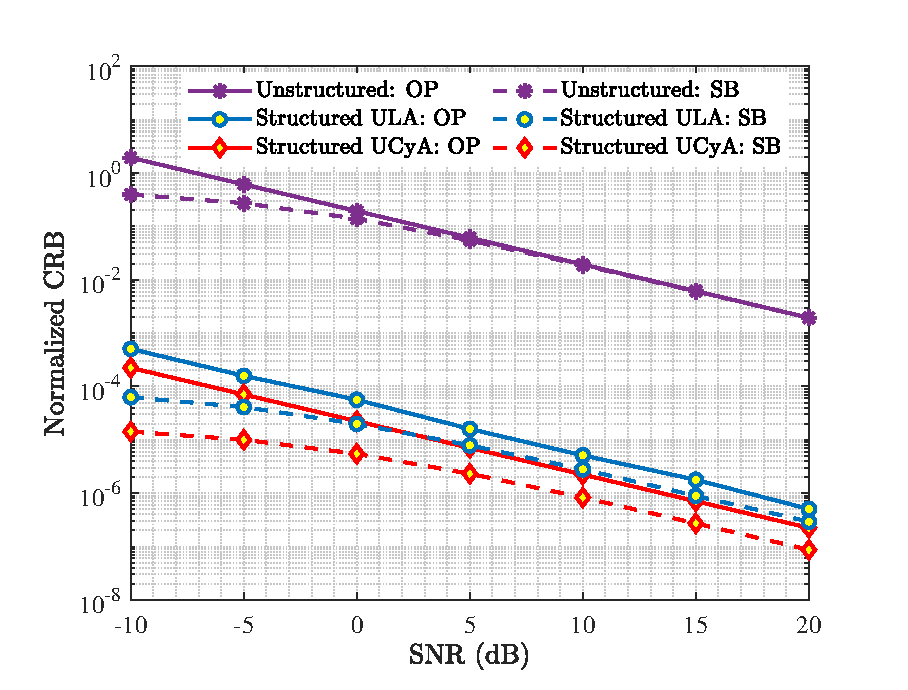
\includegraphics[width=.7\linewidth]{figures/fig_1_3.eps}
    \caption{CRB của hai cấu hình ULA và UCyA ứng với mô hình kênh truyền có cấu trúc (structured) và không sử dụng cấu trúc (unstructured). Cấu hình của mảng ăng-ten như sau $N_{ULA} = 96, N_{UCA} = 24,$ và $N_{3D} = 4$.}
    \label{fig:op}
\end{figure}

Trên hình~\ref{fig:op_N3D}, số lượng các lớp $N_{3D}$ của cấu hình UCyA được khảo sát bằng cách giữ nguyên số phần tử thuộc mảng vòng $N_{UCA} = 24$ và SNR~$=5$~dB. Có thể rút ra nhận xét thứ hai, sử dụng mô hình kênh truyền có cấu trúc và cấu hình mảng UCyA có thể cho hiệu suất ước lượng kênh truyền tốt hơn khi $N_{3D}$ nhỏ. Tuy nhiên, lưu ý rằng, ngoài lợi thế về độ chính xác, khi số lượng phần tử trong mảng lên đến $240$ như trong mô phỏng, cấu hình mảng UCyA sẽ giúp tiết kiệm được rất nhiều diện tích lắp đặt mảng ăng-ten.
\begin{figure}[H]
    \centering
    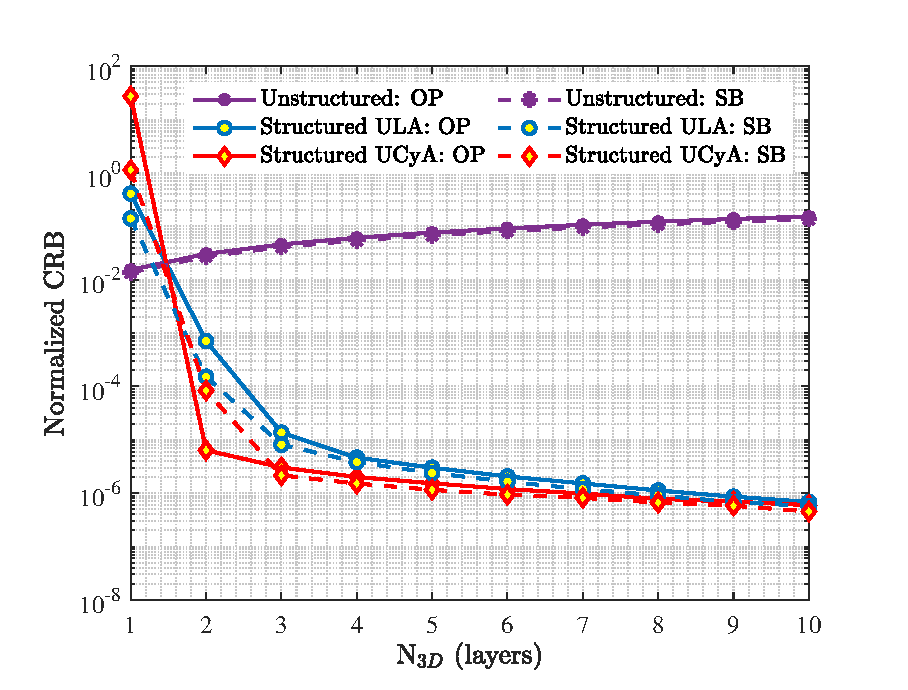
\includegraphics[width=.7\linewidth]{figures/fig_2_3.eps}
    \caption{CRB của hai cấu hình ULA và UCyA khi thay đổi $N_{3D}$. Các thông số mô phỏng như sau $N_{UCA} = 24, N_{ULA} = 24 * N_{3D}$, và SNR $=5$~dB.}
    \label{fig:op_N3D}
\end{figure}

Cuối cùng, trên hình~\ref{fig:op_NUCA}, số lượng phần tử của một mảng tròn UCA được thay đổi trong khoảng từ $8$ đến $64$ phần tử, trong khi giữ nguyên $N_{3D} = 4, N_{ULA} = 4 \times N_{UCA}$, và SNR $=5$~dB. Có thể rút ra nhận xét thứ ba, sử dụng mô hình kênh truyền có cấu trúc và cấu hình mảng UCyA có thể cho hiệu suất ước lượng kênh truyền tốt hơn và tăng dần với $N_{UCA}$. Tuy nhiên, cần lưu ý dù cho độ chính xác cao hơn, nhưng khi $N_{UCA}$ tăng cao, bán kính của mảng tròn UCA lớn dần lại dẫn đến lãng phí diện tích lắp đặt mảng ăng-ten.
\begin{figure}[ht]
    \centering
    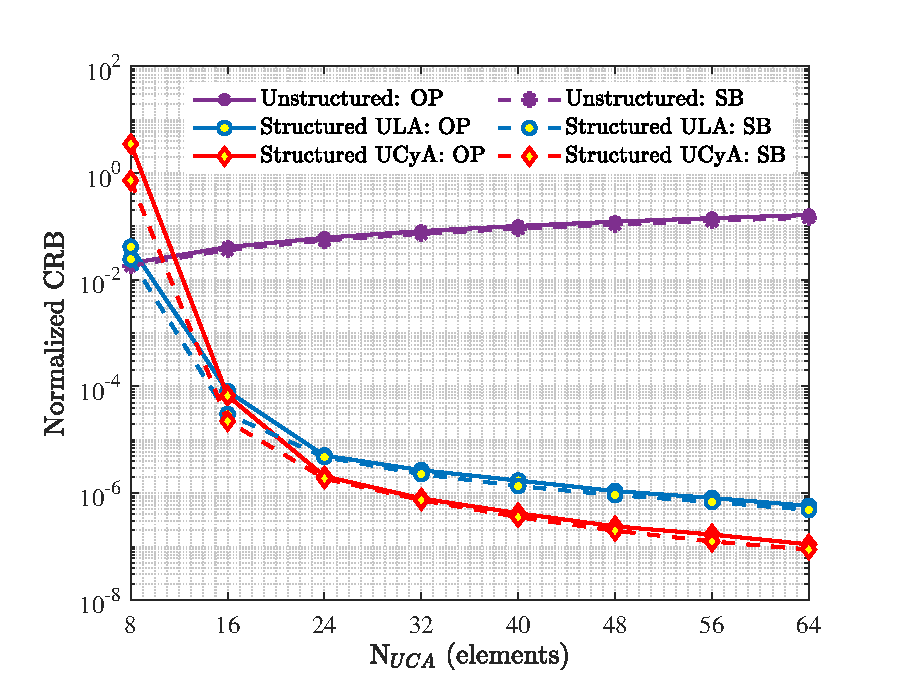
\includegraphics[width=.7\linewidth]{figures/fig_3_3.eps}
    \caption{CRB của hai cấu hình ULA và UCyA khi thay đổi $N_{UCA}$. Các thông số mô phỏng như sau $N_{3D} = 4, N_{ULA} = 4 * N_{UCA}$, và SNR $=5$~dB.}
    \label{fig:op_NUCA}
\end{figure}
\newpage
\clearpage
\phantomsection

\setcounter{chapter}{2}
\chapter[NHẬN DẠNG HỆ THỐNG SỬ DỤNG MẠNG HỌC SÂU]{Nhận dạng hệ thống sử dụng mạng học sâu}
\label{sec:ML}

% Trong chương này, tác giả đề xuất một kiến trúc mạng học sâu ISDNN sử dụng cho nhận dạng hệ thống viễn thông mMIMO. Đầu tiên, sơ lược về hai hướng tiếp cận sử dụng mạng nơ-ron sâu sẽ được giới thiệu. Kế đến là khái niệm về kỹ thuật mở rộng sâu (Deep unfolding). Một kiến trúc được mở rộng sâu từ bộ tối ưu MLE là DetNet được trình bày để so sánh ở mục các kết quả mô phỏng. Tiếp đến, từ một giải thuật ISD đã được đề xuất trong~\cite{Mandloi2017}, kết hợp với cách tiếp cận mở rộng sâu tại~\cite{Liao2020}, một mạng nơ-ron sâu tên ISDNN được đề xuất để nhận dạng hệ thống. Kiến trúc mạng ISDNN được đề xuất cho cả hai mô hình kênh truyền có cấu trúc và không sử dụng cấu trúc đã được trình bày tại chương~\ref{sec:CRB}. Các bước mô phỏng và đánh giá sẽ được đưa ra để cho thấy tiềm năng của phương pháp đề xuất và kết luận của chương. 

% \section{Giới thiệu về mạng nơ-ron sâu và mở rộng sâu}
% \begin{figure} [H]
%     \centering
%     \begin{tikzpicture}[x=2.2cm,y=1.4cm]
%         \node[antenna, thick, scale=0.6] at (5mm, 14mm) (Rx0) {};
%         \node at (5mm, 30mm) (text_Rx0) {Rx $1$};
%         \draw[line] (5mm, 14mm) -- (18mm,14mm);
    
%         \node[antenna, thick, scale=0.6] at (0mm, 0mm) (Rx1) {};
%         \node at (0mm, 16mm) (text_Rx0) {Rx $2$};
%         \draw[line] (0mm, 0) -- (18mm, 0);

%         \node[antenna, thick, scale=0.6] at (-5mm, -14mm) (Rx2) {};
%         \node at (-5mm, 2mm) (text_Rx0) {Rx $3$};
%         \draw[line] (-5mm, -14mm) -- (18mm, -14mm);
    
%         \node[scale=1.5] at (0mm, -23mm) (dotss) {$\mathbf{\vdots}$};
    
%         \node[antenna, thick, scale=0.6] at (-10mm, -35mm) (RxL) {};
%         \node at (-10mm, -19mm) (text_RxL) {Rx $L$};
%         \draw[line] (-10mm, -35mm) -- (18mm, -35mm);

    
%       \readlist\Nnod{4,5,5,5,3} % array of number of nodes per layer
%       \readlist\Nstr{L,m,m,m,T} % array of string number of nodes per layer
%       \readlist\Cstr{\strut x,a^{\prev},a^{\prev},a^{\prev}, s} % array of coefficient symbol per layer
%       \def\yshift{0.5} % shift last node for dots
      
%       \foreachitem \N \in \Nnod{ % loop over layers
%         \def\lay{\Ncnt} % alias of index of current layer
%         \pgfmathsetmacro\prev{int(\Ncnt-1)} % number of previous layer
%         \message{\lay,}
%         \foreach \i [evaluate={\c=int(\i==\N); \y=\N/2-\i-\c*\yshift;
%                      \index=(\i<\N?int(\i):"\Nstr[\lay]");
%                      \x=\lay; \n=\nstyle;}] in {1,...,\N}{ % loop over nodes
%           % NODES
%           \node[node \n] (N\lay-\i) at (\x,\y) {$\Cstr[\lay]_{\index}$};
          
%           % CONNECTIONS
%           \ifnum\lay>1 % connect to previous layer
%             \foreach \j in {1,...,\Nnod[\prev]}{ % loop over nodes in previous layer
%               \draw[connect,white,line width=1.2] (N\prev-\j) -- (N\lay-\i);
%               \draw[connect] (N\prev-\j) -- (N\lay-\i);
%               %\draw[connect] (N\prev-\j.0) -- (N\lay-\i.180); % connect to left
%             }
%           \fi % else: nothing to connect first layer
          
%         }
%         \path (N\lay-\N) --++ (0,1+\yshift) node[midway,scale=1.5] {$\vdots$};
%       }
      
%       % LABELS
%       \node[above=2,align=center,green!60!black] at (1, 0) {Đầu vào};
%       \node[above=2,align=center,blue!60!black] at (65mm, 0) {Lớp ẩn};
%       \node[above=2,align=center,red!60!black] at (110mm, 0) {Đầu ra};
      
%     \end{tikzpicture}
%     \caption{Minh họa sử dụng DNN để nhận dạng hệ thống viễn thông.}
%     \label{fig:DNN_model}
% \end{figure}
% Trong chương~\ref{sec:back}, các phương pháp nhận dạng hệ thống sử dụng các phương pháp ML/DL được chia làm ba loại, trong đó phương pháp sử dụng các mạng nơ-ron đang được quan tâm nghiên cứu. Các mạng nơ-ron sâu được sử dụng rộng rãi trong các ứng dụng như xử lý tiếng nói, ngôn ngữ tự nhiên, hình ảnh, thị giác máy, trò chơi trực tuyến~\cite{Samek2021}. Mười năm trở lại đây, đã có nhiều nghiên cứu ứng dụng các mạng DNN khác nhau cho vấn đề nhận dạng hệ thống viễn thông không dây. Hình~\ref{fig:DNN_model} biểu diễn mô hình minh họa việc sử dụng DNN để ước lượng kênh truyền và khôi phục tín hiệu gốc. Có thể chia các phương pháp này thành hai hướng tiếp cận, bao gồm hướng dữ liệu (data-driven) và hướng mô hình (model-driven)~\cite{Liao2020}. Các phương pháp data-driven trực tiếp học các đặc trưng từ một tập lớn các dữ liệu (dataset) để phục vụ cho các mục đích như ước lượng kênh truyền, phản hồi CSI,~\ldots Tuy các phương pháp data-driven đều cho độ chính xác cao nhưng vẫn có những thách thức khi yêu cầu số lượng mẫu rất lớn và kéo theo đó là thời gian/chi phí cho việc đào tạo lớn. Các phương pháp model-driven~\cite{He2019} có thể khắc phục một phần các hạn chế này bằng việc tối ưu/đưa thêm các tham số học vào các kiến trúc có sẵn để kết hợp ưu điểm của data-driven và các mô hình toán học truyền thống. 

% Gần đây, kỹ thuật mở rộng sâu~\cite{Wisdom2016} là một giải pháp tiềm năng để chuyển các giải thuật truyền thống thành các kiến trúc mạng DNN theo hướng tiếp cận model-driven. Chi tiết về mở rộng sâu được trình bày tại~\cite{John2014}, các phương pháp yêu cầu các vòng lặp đi lặp lại (iteractive inference) có thể dễ dàng chuyển đổi sang các lớp của một mạng NN. Sau đó, sử dụng các giải thuật giảm dần độ dốc (GD - Gradient Descent) để đào tạo tham số trên các lớp mạng. Sau $K$ lớp đào tạo tương tự như $K$ vòng lặp trong thuật toán gốc, mô hình có thể đạt được mục tiêu mong muốn. Ví dụ, DetNet~\cite{Samuel2017} là một mạng DNN dựa trên việc mở rộng sâu bộ nhận dạng MLE và sử dụng giảm dần độ dốc dự kiến (PGD - Projected Gradient Descent)~\cite{Chen2015}. Trong mục tiếp theo, mạng nơ-ron sâu DetNet sẽ được giới thiệu ngắn gọn và kết quả của DetNet sẽ được so sánh với kiến trúc mạng đề xuất.

\section{Mạng nơ-ron sâu DetNet}

Vẫn sử dụng mô hình hệ thống mMIMO đã trình bày ở phần~\ref{sec:mMIMO}.
\begin{equation}
    \mathbf{x} = \mathbf{H} \mathbf{s} + \mathbf{w}
\end{equation}
Các phần tử trong ma trận kênh truyền $\mathbf{H}$ được biểu diễn dưới dạng số phức, đại diện cho cả ảnh hưởng về biên độ và pha gây ra bởi kênh. Cách biểu diễn này phù hợp trên lý thuyết, các phương pháp giải tối ưu, và các phần mềm mô phỏng như Matlab. Tuy nhiên, trong học máy/học sâu, các giá trị số phức thường được tách riêng thành phần thực ($\Re$) và phần ảo ($\Im$) như sau:
% riêng biệt.
% Quá trình học của thành phần thực và ảo thuộc một giá trị số phức cũng được tách riêng biệt, qua đó phát huy lợi thế của ML/DL.
% Bên cạnh đó, các phép toán phổ biến trong xử lý tín hiệu như chuyển vị, liên hợp phức cũng sẽ được thực hiện dễ dàng hơn nếu tách riêng thành phần thực và ảo.
% Từ các lý do trên, các phương pháp sử dụng ML/DL nhận dạng kênh sẽ chuyển đổi tất cả các giá trị phức sang dạng thực trước khi đưa vào quá trình đào tạo trong mạng. Các mạng ML/DL này thường được phát triển trên ngôn ngữ Python và các thư viện nền tảng thông dụng như Tensorflow\footnote{\url{https://github.com/tensorflow/tensorflow}} của Google hay Pytorch\footnote{\url{https://github.com/pytorch/pytorch}} của Facebook. 
% % Do vậy, không làm mất đi tính tổng quát, trong chương này, 
% Các ma trận và véc-tơ trên mô hình kênh kể trên sẽ được biểu diễn dưới dạng các thành phần thực ($\Re$) và phần ảo ($\Im$) như sau:
\begin{equation}
\label{eq:matrixtras1}
    \mathbf{s}=\left[\begin{array}{l}
    \Re(\mathbf{s}) \\
    \Im(\mathbf{s})
    \end{array}\right] ;
    \mathbf{x}=\left[\begin{array}{l}
    \Re(\mathbf{x}) \\
    \Im(\mathbf{x})
    \end{array}\right] ; 
    \mathbf{w}=\left[\begin{array}{l}
    \Re(\mathbf{w}) \\
    \Im(\mathbf{w})
    \end{array}\right]
\end{equation}

\begin{equation}
\label{eq:matrixtras2}
    \mathbf{H}=\left[\begin{array}{cc}
    \Re(\mathbf{H}) & -\Im(\mathbf{H}) \\
    \Im(\mathbf{H}) & \Re(\mathbf{H})
    \end{array}\right]
\end{equation}
trong đó, $\mathbf{H} \in \mathbb{R}^{2L \times 2T}$, $\mathbf{s} \in \mathbb{R}^{2T \times 1}$, $\mathbf{w} \in \mathbb{R}^{2L \times 1}$, và $\mathbf{x} \in \mathbb{R}^{2L \times 1}$. Thông thường, các kiến trúc mạng ML/DL sử dụng để ước lượng kênh truyền giả sử rằng ma trận kênh truyền $\mathbf{H}$ được mô hình hoá dưới dạng không sử dụng cấu trúc, hay các hệ số của $\mathbf{H}$ được chọn ngẫu nhiên và không bị ảnh hưởng bởi các thông số vật lý khác như DoA, cấu hình mảng ăng-ten,~\ldots Để tìm bộ nhận dạng cho hệ thống kể trên, định nghĩa hàm mất mát $\mathcal{L}\left(\mathbf{s} ; \hat{\mathbf{s}}_{\boldsymbol{\Theta}}(\mathbf{H}, \mathbf{x})\right)$ là khoảng cách giữa véc-tơ ký hiệu gốc và véc-tơ ký hiệu được ước lượng. Tìm giá trị $\boldsymbol{\Theta}$ bằng cách tối thiểu hoá hàm mất mát kể trên như sau:
\begin{equation}
\label{eq:lossf}
\min _{\boldsymbol{\Theta}} \mathbb{E}\left\{\mathcal{L}\left(\mathbf{s} ; \hat{\mathbf{s}}_{\boldsymbol{\Theta}}(\mathbf{H}, \mathbf{x})\right)\right\}
\end{equation}

Sử dụng giải thuật MLE để giải~(\ref{eq:lossf}) được:
\begin{equation}
\label{eq:mle}
\hat{\mathbf{s}}_{\boldsymbol{\Theta}}(\mathbf{H}, \mathbf{x})=\arg \min _{\mathbf{s} \in \mathbb{R}^{2T}}\|\mathbf{x}-\mathbf{H} \mathbf{s}\|^2
\end{equation}
% Tuy nhiên, độ phức tạp của MLE sẽ tăng theo cấp số mũ $\mathcal{O}(2^T)$ nên khó để triển khai trong các hệ mMIMO. Do vậy, DetNet được đề xuất nhằm tạo ra một kiến trúc mạng DNN tiệm cận độ chính xác với MLE. Trong nghiên cứu gốc, thay vì tạo ra một mạng nơ-ron nhằm ánh xạ trực tiếp từ $\mathbf{x}$ về $\mathbf{s}$, việc phân tách $\mathbf{x}$ thành các thành phần $\mathbf{H}, \mathbf{s},$ và $\mathbf{w}$ như~(\ref{eq:3.6}) sẽ cho hiệu quả cao hơn.
% \begin{equation}
%     \label{eq:3.6}
%     \mathbf{H}^\top \mathbf{x}=\mathbf{H}^\top \mathbf{H s}+\mathbf{H}^\top \mathbf{w}
% \end{equation}

DetNet dựa trên phương pháp PGD thực hiện việc tối ưu MLE như phương trình~(\ref{eq:mle}).
% Đạo hàm riêng được tách như trên (\ref{eq:pgd}) sử dụng luật chuỗi (chain rule).
% \begin{equation}
% \label{eq:pgd}
%     \begin{aligned}
%     \hat{\mathbf{s}}_{k+1} & =\boldsymbol{\Gamma}\left[\hat{\mathbf{s}}_k-\left.\delta_k \frac{\partial\|\mathbf{x}-\mathbf{H} \mathbf{s}\|^2}{\partial \mathbf{s}}\right|_{\mathbf{s}=\hat{\mathbf{s}}_k}\right] \\
%     & = \boldsymbol{\Gamma}\left[\hat{\mathbf{s}}_k-\delta_k \mathbf{H}^\top \mathbf{x}+\delta_k \mathbf{H}^\top \mathbf{H} \hat{\mathbf{s}}_k\right]
%     \end{aligned}
% \end{equation}
% với $\hat{\mathbf{s}}_k$ là véc-tơ giá trị nguồn ước lượng tại lớp thứ $k$, $\boldsymbol{\Gamma}[.]$ là một phép biến đổi phi tuyến tính, và $\delta_k$ là độ dài bước của quá trình học. 
Kiến trúc của một lớp mạng DetNet được biểu diễn dưới dạng ma trận là:
\allowdisplaybreaks
\begin{subequations}
\begin{alignat}{4}
    \mathbf{z}_k & =\rho\left(\mathbf{W}^1_{k}\left[\begin{array}{c}
    \mathbf{H}^\top \mathbf{x} \\
    \hat{\mathbf{s}}_k \\
    \mathbf{H}^\top \mathbf{H} \hat{\mathbf{s}}_k \\
    \mathbf{v}_k
    \end{array}\right]+\mathbf{b}^1_{k}\right) \\
    \hat{\mathbf{s}}_{k+1} & =\psi_{t_k}\left(\mathbf{W}^2_{k} \mathbf{z}_k+ \mathbf{b}^2_{k}\right) \\
    {\mathbf{v}}_{k+1} & =\mathbf{W}^3_{k} \mathbf{z}_k+ 
    \mathbf{b}^3_{k} \\
    \hat{\mathbf{s}}_1 & =\mathbf{0}_{2T}
\end{alignat}
\end{subequations}
trong đó, $k = 1, \ldots, K$ là số các lớp của mạng DetNet, $\rho$ là một toán tử tuyến tính. $\psi_{t_k}$ ký hiệu cho phép biến đổi phi tuyến tính phân đoạn, ở các mức $t$ khác nhau, $\psi_{t_k}(s)$ có biểu diễn toán học như sau:
\begin{equation}
    \psi_{t_k}(s)=-1+\frac{\rho\left(s + t_k \right)}{\left|t_k\right|}-\frac{\rho\left(s- t_k \right)}{\left|t_k\right|}
\end{equation}

% \begin{figure}[tb]
%     \centering
%     \begin{tikzpicture}
%         \node (B11) [field6, fill=red!10!white] at (0, 0) {$\mathbf{H}^\top \mathbf{x}$};
%         \node (B21) [below=10mm of B11, field6, fill=red!10!white] {$\mathbf{v}_k$};
%         \node (B31) [below=10mm of B21, field6, fill=red!10!white] {$\hat{\mathbf{s}}_k$};
%         \node (B41) [below=10mm of B31, field6, fill=red!10!white] {$\mathbf{H}^\top \mathbf{H}$};

        
%         \node (B32) [right=10mm of B31.south east, anchor=north, circle, fill=blue!10!white, draw=black] {$\times$}; 
%         \node (B22) [right=25mm of B21, circle, fill=blue!10!white, draw=black] {$\operatorname{con}$};
%         \node (B33) [below=11mm of B22, circle, fill=blue!10!white, draw=black] {$\times$};
%         \node (B34) [below=4mm of B33, field8, fill=green!10!white, draw=black] {$\mathbf{W}^1_{k}$};
%         \node (B35) [right=7mm of B33, circle, fill=blue!10!white, draw=black] {$+$};
%         \node (B36) [below=4mm of B35, field8, fill=green!10!white, draw=black] {$\mathbf{b}^1_{k}$};

%         \node (B37) [circle, fill=blue!10!white, draw=black] at (70mm, -30mm) {$\rho$};
%         \node (B38) [right=40mm of B33, circle, fill=blue!10!white, draw=black] {$\times$};
%         \node (B39) [below=4mm of B38, field8, fill=green!10!white, draw=black] {$\mathbf{W}^2_{k}$};
%         \node (B310) [right=7mm of B38, circle, fill=blue!10!white, draw=black] {$+$};
%         \node (B311) [below=4mm of B310, field8, fill=green!10!white, draw=black] {$\mathbf{b}^2_{k}$};
%         \node (B312) [right=7mm of B310, circle, fill=blue!10!white, draw=black] {$\Psi$};

%         \node (B23) [above=24.2mm of B39, circle, fill=blue!10!white, draw=black] {$\times$};
%         \node (B24) [right=7mm of B23, circle, fill=blue!10!white, draw=black] {$+$};
%         \node (B25) [above=4mm of B23, field8, fill=green!10!white, draw=black] {$\mathbf{W}^3_{k}$};
%         \node (B26) [above=4mm of B24, field8, fill=green!10!white, draw=black] {$\mathbf{b}^3_{k}$};

%         \node (Bvk1) [right=123mm of B21, field6, fill=red!10!white] {$\mathbf{v}_{k+1}$};
%         \node (Bxk1) [right=123mm of B31, field6, fill=red!10!white] {$\hat{\mathbf{s}}_{k+1}$};

%         \draw[arrow] (B312) -- (Bxk1);
%         \draw[arrow] (B24) -- (Bvk1);
%         \draw[arrow] (B310) -- (B312);
%         \draw[arrow] (B38) -- (B310);
%         \draw[arrow] (B23) -- (B24);
%         \draw[arrow] (B25) -- (B23);
%         \draw[arrow] (B26) -- (B24);
%         \draw[arrow] (B311) -- (B310);
%         \draw[arrow] (B39) -- (B38);
%         \draw[arrow] (B33) -- (B35);
%         \draw[arrow] (B36) -- (B35);
%         \draw[arrow] (B34) -- (B33);
%         \draw[arrow] (B22) -- (B33);

%         \draw[arrow] (B21) -- (B22);
%         \draw[line] (B11) -- ([yshift=-3mm]B11.south);
%         \draw[arrow] ([yshift=-3mm]B11.south) -| (B22);
%         \draw[line] (B31) -- ([xshift=3mm]B31.east);
%         \draw[arrow] ([xshift=3mm]B31.east) |- ([yshift=-1.5mm]B22.west);
%         \draw[line] (B32) -- ([xshift=3mm]B32.east);
%         \draw[arrow] ([xshift=3mm]B32.east) |- ([yshift=-3mm]B22.west);

%         \draw[arrow] (B31) |- ([yshift=3mm]B32);
%         \draw[arrow] (B41) |- ([yshift=-3mm]B32);

%         \draw[arrow] (B37) |- (B38);
%         \draw[arrow] (B37) |- (B23);
%         \draw[arrow] (B35) |- (B37);
        
%         \draw[arrow] (B41) -- (150mm, -60mm);
%         \draw[arrow] (Bvk1) -- (150mm, -20mm);
%         \draw[arrow] (Bxk1) -- (150mm, -41mm);
%         \draw[arrow] (B11) -- (150mm, 0mm);

%         % Legends
%         \node[rectangle, draw=black, dashed, fill=black!5!white, minimum width=140mm, minimum height=35mm] at (70mm, -85mm) {};

%         \node (B51) [field6, fill=red!10!white] at (22mm, -78mm) {Giá trị \\đầu vào/đầu ra};

%         \node (B61) [below=4mm of B51, field8, fill=green!10!white, draw=black] {Giá trị học};

%         \node (B52) [right=7mm of B51, circle, fill=blue!10!white, draw=black] {$\times$};
%         \draw[arrow] (B52) -- ([xshift=3mm]B52.east) node [pos=0, right=3mm] {Nhân};

%         \node (B53) [below=7mm of B52, circle, fill=blue!10!white, draw=black] {$+$};
%         \draw[arrow] (B53) -- ([xshift=3mm]B53.east) node [pos=0, right=3mm] {Cộng};

%         \node (B54) [right=20mm of B52, circle, fill=blue!10!white, draw=black] {$\rho$};
%         \draw[arrow] (B54) -- ([xshift=10mm]B54.east) node [pos=0, right=10mm, above, label={below}:{tuyến tính}] {Toán tử};

%         \node (B55) [right=20mm of B53, circle, fill=blue!10!white, draw=black] {$\Psi$};
%         \draw[arrow] (B55) -- ([xshift=10mm]B55.east) node [pos=0, right=11mm, above, label={below}:{phi tuyến tính}] {Toán tử};

%         \node (B56) [right=28mm of B54, circle, fill=blue!10!white, draw=black] {$\operatorname{con}$};
%         \draw[arrow] (B56) -- ([xshift=10mm]B56.east) node [pos=0, right=11mm, above, label={below}:{véc-tơ}] {Nối};
         
%     \end{tikzpicture}
%     \caption{Kiến trúc của một lớp trong kiến trúc mạng DetNet~\cite{Samuel2017}.}
%     \label{fig:detnet}
% \end{figure}

% \begin{figure}[ht]
%     \centering
%     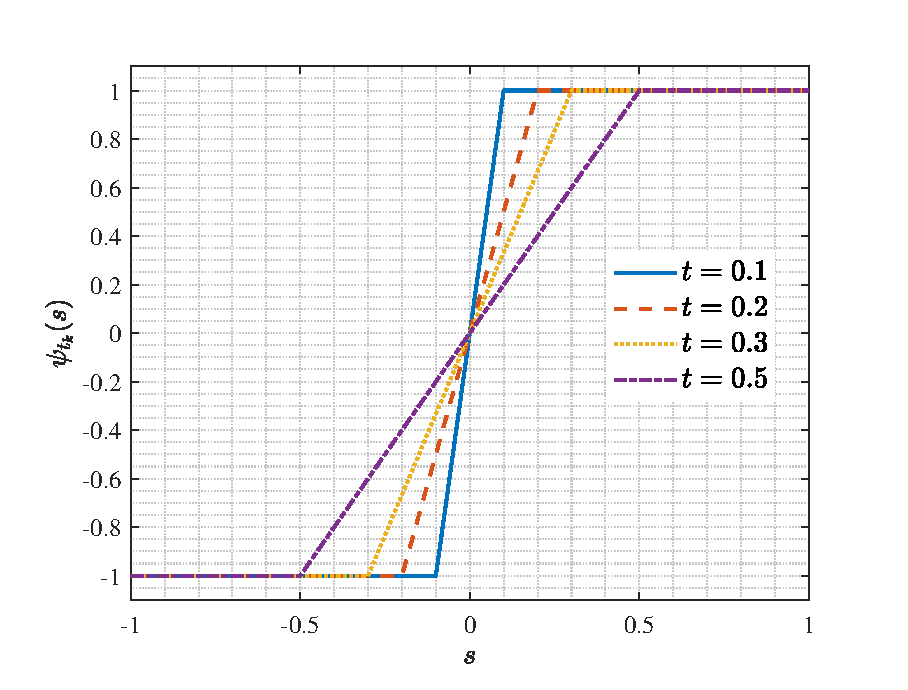
\includegraphics[width=.8\linewidth]{figures/soft_sign.eps}
%     \caption{Hàm phi tuyến tính phân đoạn $\psi_{t_k}(s)$ được sử dụng trong DetNet.}
%     \label{fig:soft_sign}
% \end{figure}
Các tham số của việc học sẽ bao gồm:
\begin{equation}
\boldsymbol{\Theta}=\left\{\mathbf{W}^1_{k}, \mathbf{b}^1_{k}, \mathbf{W}^2_{k}, \mathbf{b}^2_{k}, \mathbf{W}^3_{k}, \mathbf{b}^3_{ k}, t_k\right\}_{k=1}^K
\end{equation}

Sau mỗi vòng lặp (iteration), một hàm mất mát có dạng sai số bình phương trung bình (MSE - Mean Squared Error) sẽ tính toán sự sai khác của véc-tơ các ký hiệu ước lượng so với véc-tơ các ký hiệu gốc. Kết quả này được sử dụng để xem xét sự hội tụ của việc đào tạo, và được trả về cho giải thuật tối ưu (ví dụ: Adam) để tối ưu các tham số học của mạng. Hàm mất mát này được định nghĩa như dưới đây:
\begin{equation}
\label{eq:lossdetnet}
    \mathcal{L}(\mathbf{s} ; \hat{\mathbf{s}}_{\boldsymbol{\Theta}}(\mathbf{H}, \mathbf{x}))= \frac{1}{2T} \sum_{t=1}^{2T} {\left\| s_t-\hat{s}_t\right\|^2}
\end{equation}
% \begin{equation}
% \label{eq:lossdetnet}
%     l(\mathbf{s} ; \hat{\mathbf{s}}(\mathbf{H}, \mathbf{x}))=\sum_{k=1}^K \log (k) \frac{\left\|\mathbf{s}-\hat{\mathbf{s}}_k\right\|^2}{\|\mathbf{s}-\tilde{\mathbf{s}}\|^2}
% \end{equation}
% với $\tilde{\mathbf{s}}$ là ước lượng của $\mathbf{s}$ thu được từ bộ giải mã ZF như trình bày trong mục~\ref{sec:zf}. Lưu ý rằng, do $\mathbf{H}$ là ma trận của các số thực nên phép chuyển vị liên hợp phức $(.)^H$ sẽ được chuyển thành chuyển vị $(.)^\top$.
% \begin{equation}
%     \tilde{\mathbf{s}}=\left(\mathbf{H}^\top \mathbf{H}\right)^{-1} \mathbf{H}^\top \mathbf{x}
% \end{equation}

\section{Đề xuất mạng nơ-ron sâu ISDNN cho nhận dạng kênh truyền}
\subsection{Bộ nhận dạng ISD cho hệ thống mMIMO}

Bài báo đã đề xuất một bộ nhận dạng kênh truyền tuần tự lặp lại gọi tắt là ISD để đạt được hiệu suất của MMSE với độ phức tạp thấp.
\begin{equation}
    \hat{\mathbf{s}}_{MMSE}=\left(\mathbf{H}^\top \mathbf{H}+\frac{\sigma^2}{\mathbb{E}(\mathbf{s})} \mathbf{I}_{2T}\right)^{-1} \mathbf{H}^\top \mathbf{x}=\mathbf{P}^{-1} \mathbf{q}
\end{equation}
ký hiệu $\mathbf{G}_\mathbf{H} = \mathbf{H}^\top \mathbf{H}$, $\mathbf{P} = \mathbf{H}^\top \mathbf{H}+\frac{\sigma^2}{\mathbb{E}(\mathbf{s})} \mathbf{I}_{2T}$, và $\mathbf{q} = \mathbf{H}^\top \mathbf{x}$. 
Các thành phần đường chéo của ma trận $\mathbf{P}$ tạo thành ma trận đường chéo $\mathbf{D} = \operatorname{diag}(\mathbf{P})$.
% Định nghĩa ma trận $\mathbf{P}$ tạo thành ma trận $\mathbf{D} = \operatorname{diag}(\mathbf{H}^\top \mathbf{H})$.
Lưu ý, độ phức tạp của việc nghịch đảo $\mathbf{P}$ là $\mathcal{O}(TL^3)$, sẽ tăng nhanh khi $L$ lớn. 

Để đạt được hiệu năng cao hơn với số lần lặp ít hơn, ISD đề xuất khởi tạo véc-tơ của các ký hiệu ước lượng ($\hat{\mathbf{s}}_1$) như trên phương trình~(\ref{eq:sinit}) thay vì đặt tất cả bằng $0$ như DetNet.
\begin{equation}
\label{eq:sinit}
    \hat{\mathbf{s}}_1=\mathbf{D}^{-1} \mathbf{q}=\left[s_1(1), s_1(2), \ldots, s_1(2T)\right]
\end{equation}

% Từ véc-tơ tín hiệu thu, tín hiệu của ăng-ten/người dùng thứ $j$ thu được bằng cách coi tín hiệu từ các ăng-ten/người dùng khác như tạp âm và loại bỏ chúng.
% \begin{equation}
%     \hat{\mathbf{x}}(j)=\mathbf{x}-\sum_{t=1, t \neq j}^{2T} \mathbf{h}_t \hat{s}_k(t)
% \end{equation}
% với $\hat{\mathbf{x}}(j)$ thu được, ký hiệu được gửi từ người dùng thứ $j$ được ước lượng như sau:
% \begin{equation}
% \label{eq:supdate}
%     \begin{aligned}
%         \hat{s}_{k+1}(j) & =\frac{\mathbf{h}_j^\top}{\left\|\mathbf{h}_j\right\|^2} \hat{\mathbf{x}}(j) \\ 
%         & = \hat{s}_k(j)+\frac{1}{\mathbf{G}_\mathbf{H}(j, j)}\left(\mathbf{q}(j)-\sum_{t=1}^{2T} \mathbf{G}_\mathbf{H}(j, t) s_k(t)\right)
%     \end{aligned}
% \end{equation}
% trong đó, $\mathbf{h}_j$ là cột thứ $j$ của ma trận $\mathbf{H}$, $\mathbf{G}_\mathbf{H}(i, j)$ là phần tử thứ $(i, j)$ của ma trận $\mathbf{G}_\mathbf{H}$, và $\mathbf{q}(j)$ là phần tử thứ $j$ của véc-tơ $\mathbf{q}$.
Véc-tơ các ký hiệu ước lượng $\hat{\mathbf{s}}$ được cập nhật như trong thuật toán~\ref{alg:cap} của giải thuật ISD. 
\begin{algorithm}[ht]
    \caption{Bộ nhận dạng Iterative Sequential.}\label{alg:cap}
    \hspace*{\algorithmicindent} \textbf{Input: $\mathbf{x}, \mathbf{H}, L, T, K, \sigma^2, \mathbb{E}(\mathbf{s})$} \\
    \hspace*{\algorithmicindent} \textbf{Output: $\hat{\mathbf{s}}_{out} = \hat{\mathbf{s}}^{2T}_K$} 
    \begin{algorithmic}[1]
        \State $\mathbf{G}_\mathbf{H} \leftarrow \mathbf{H}^\top \mathbf{H}$
        \State $\mathbf{P} \leftarrow \mathbf{G}_\mathbf{H} + \frac{\sigma^2}{\mathbb{E}(\mathbf{s})} \mathbf{I}_{2T}$
        \State $\mathbf{D} \leftarrow \operatorname{diag}(\mathbf{P})$
        \State $\mathbf{q} \leftarrow \mathbf{H}^\top \mathbf{x}$
        \State $\mathbf{s}_1 \leftarrow \mathbf{D}^{-1} \mathbf{q}$ \\
        \For{ $k=0, k < K$}
            \For{ $j=1, j \le 2T$}
                \State $\hat{s}_k(j+1) \leftarrow \hat{s}_k(j)+\frac{1}{\mathbf{G}_\mathbf{H}(j, j)}\left(\mathbf{q}(j)-\sum_{t=1}^{2T} \mathbf{G}_\mathbf{H}(j, t) \hat{s}_k(t)\right)$ \\ 
                \State $\hat{\mathbf{s}}_{k+1}^j \leftarrow\left[\hat{s}_{k+1}(1),~\ldots, \hat{s}_{k+1}(j), \hat{s}_k(j+1),~\ldots, \hat{s}_k(2T)\right]$
                \State $j \leftarrow j + 1$
            \EndFor
            \State $k \leftarrow k + 1$
        \EndFor
    \end{algorithmic}
\end{algorithm}

Để chứng minh giải thuật ISD là hiệu quả cho việc ước lượng kênh truyền, véc-tơ phần dư (sai số) sẽ được sử dụng. Cụ thể, véc-tơ phần dư thu được sau khi khởi tạo với các giá trị $\hat{\mathbf{s}}_1$ là:
\begin{equation}
    \mathbf{e}_1 = \mathbf{x} - \mathbf{H} \hat{\mathbf{s}}_1
\end{equation}
từ đó, véc-tơ phần dư sau khi cập nhật ký hiệu thứ $j$ tại lớp thứ $k$ sẽ được biểu diễn như sau:
\begin{equation}
    \mathbf{e}_k^{j}=\mathbf{x}-\mathbf{H} \hat{\mathbf{s}}_k^j
\end{equation}
thay $\hat{\mathbf{s}}_k^j$ bằng các biểu diễn hồi quy như trong giải thuật~\ref{alg:cap} thu được:
\begin{equation}
\label{eq:eupdate}
\begin{aligned}
    \mathbf{e}_k^{j} =\mathbf{e}_k^{j-1}-\mathbf{h}_{j} \frac{\mathbf{h}_j^\top}{\left\|\mathbf{h}_j\right\|^2} \mathbf{e}_k^{j-1}
    \end{aligned}
\end{equation}

Trong bài báo gốc, Mandloi M. và các cộng sự đã chứng minh rằng $\left\|\mathbf{e}_k^{j}\right\|^2<\left\|\mathbf{e}_k^{j-1}\right\|^2$. 
% Điều đó chỉ ra, mỗi khi ký hiệu thứ $j$ được cập nhật, véc-tơ phần dư sẽ được chiếu lên mặt phẳng `null' của cột thứ $j$ thuộc ma trận $\mathbf{H}$. Hay véc-tơ phần dư sẽ trực giao với $\mathbf{h}_j$, do đó $l_2-\operatorname{norm}$ bình phương của véc-tơ lỗi sẽ giảm sau mỗi lần ký hiệu $j$ được cập nhật cho đến khi véc-tơ $\mathbf{e}$ trực giao với không gian con kéo dài bởi cột của ma trận $\mathbf{H}$.

\subsection{Đề xuất mạng nơ-ron sâu ISDNN cho mô hình kênh truyền không sử dụng cấu trúc}
\label{sec:ISNN_nonstructured}

Từ giải thuật ISD được trình bày ở trên, theo hướng tiếp cận model-driven và kỹ thuật mở rộng sâu, một kiến trúc mạng nơ-ron sâu có tên ISDNN (Iterative Sequential Deep-neural Network) tương ứng cho mô hình kênh truyền không sử dụng cấu trúc (gọi tắt là \textbf{ISDNN không sử dụng cấu trúc}) được đề xuất. Đầu tiên, việc cập nhật các ký hiệu $\mathbf{s}$ tại dòng $9$ của giải thuật~\ref{alg:cap} được viết lại dưới dạng ma trận như sau:
\begin{equation}
\hat{\mathbf{s}}_{k+1}=\hat{\mathbf{s}}_k+\mathbf{e}_{k+1}
\end{equation}
trong đó, $\mathbf{e}_{k+1}$ là véc-tơ phần dư cũng được viết dưới dạng ma trận là:
\begin{equation}
    \mathbf{e}_{k+1}=\mathbf{D}^{-1}\left(\mathbf{H}^\top \mathbf{x}-\mathbf{H}^\top \mathbf{H} \hat{\mathbf{s}}_k\right)
\end{equation}
với ma trận đường chéo $\mathbf{D}$ được đơn giản hoá lấy ý tưởng từ bộ nhận dạng ZF khi không có thông tin về SNR tại bên thu, tức nghịch đảo của ma trận Gram ($\mathbf{G}_\mathbf{H}$), $\mathbf{D}~=~\operatorname{diag}(\mathbf{H}^\top \mathbf{H})$. 
% Việc thay đổi này làm giảm độ phức tạp của phép nghịch đảo $\mathbf{D}$. 
Nhận thấy rằng, $\hat{\mathbf{s}}_{k+1}$ không chỉ chịu ảnh hưởng trực tiếp bởi $\mathbf{e}_{k+1}$ mà còn tất cả các véc-tơ phần dư trước đó $\mathbf{e}_{k}, \mathbf{e}_{k-1},~\ldots, \mathbf{e}_{1}$ như biểu diễn ở công thức~(\ref{eq:eupdate}). Do vậy, để đạt được hiệu quả cao hơn trong việc loại bỏ tạp âm từ các người dùng khác, các tham số học được thêm vào $\alpha^1$ vào mỗi lớp (layer) của mạng nơ-ron.
\begin{equation}
\label{eq:supdate1}
\hat{\mathbf{s}}_{k+1}=\hat{\mathbf{s}}_k+\mathbf{e}_{k+1}+\alpha_k^{1} \mathbf{e}_k+\alpha_{k-1}^{1} \mathbf{e}_{k-1}+\cdots+\alpha_1^{1} \mathbf{e}_1
\end{equation}

Tuy nhiên, do mối tương quan giữa các véc-tơ phần dư liền kề là lớn nhất, nên trong mạng ISDNN chỉ xem xét ảnh hưởng của $\mathbf{e}_k$ ở lớp thứ $k$ nhằm đơn giản hoá kiến trúc mạng. Phương trình~(\ref{eq:supdate1}) trở thành:
\begin{equation}
\boldsymbol{\mu}_{k}=\hat{\mathbf{s}}_k+\mathbf{e}_{k+1}+\alpha_k^1 \mathbf{e}_k
\end{equation}

Thay vì gán trực tiếp $\hat{\mathbf{s}}_{k+1} = \boldsymbol{\mu}_k$, sự tương quan giữa $\boldsymbol{\mu}_k$ và $\hat{\mathbf{s}}_k$ được xem xét trước khi đưa làm đầu vào của lớp tiếp theo. Sử dụng kết hợp lồi (convex combination) của $\hat{\mathbf{s}}_k$ và $\boldsymbol{\mu}_k$ với hệ số $\alpha^2$. Do đó, $\hat{\mathbf{s}}_{k+1}$ chịu ảnh hưởng bởi cả $\hat{\mathbf{s}}_k$ và $\boldsymbol{\mu}_k$ theo tỷ lệ $\alpha^2$. 
Trong đó, $\alpha^2_k$ là tham số có thể học, $\sum_{i=k}^{k+1} \alpha_i^{2} \hat{\mathbf{s}}_i$ với $\sum_{i=k}^{k+1} \alpha_i^{2}=1$, tại mỗi lớp. Kết hợp tuyến tính của $\hat{\mathbf{s}}_k$ và $\boldsymbol{\mu}_k$ có dạng như sau:
\begin{equation}
\hat{\mathbf{s}}_{k+1}=\left(1-\alpha_k^2\right) \boldsymbol{\mu}_k + \alpha_k^2 \hat{\mathbf{s}}_k
\end{equation}

Ngoài ra, để đạt được độ chính xác cao hơn ở các loại điều chế bậc cao như (16-QAM, 64-QAM,~\ldots), véc-tơ phần dư sẽ được điều chỉnh linh hoạt hơn bằng cách thêm hai bộ biến đổi tuyến tính vào kiến trúc mạng ISDNN để cập nhật $\mathbf{e}_k$ trước khi nhân với $\alpha^1_k$.
\begin{equation}
\mathbf{e}_k \leftarrow w^2_{k}\left(w^1_{k} \mathbf{e}_k+b^1_{k}\right)+b^2_{k}
\end{equation}

Bộ nhận dạng trong các các nghiên cứu trước đây tuần tự đưa các dữ liệu huấn luyện chỉ ứng với một lần tạo dữ liệu độc lập qua mạng, tức $\mathbf{H} \in \mathbb{R}^{2L \times 2T}$, $\mathbf{s} \in \mathbb{R}^{2T \times 1}$, và $\mathbf{x} \in \mathbb{R}^{2L \times 1}$. Điều này làm giảm đáng kể tốc độ học của một mạng DNN do không tận dụng được lợi thế của kiểu dữ liệu ten-sơ (tensor), cho phép thao tác với các biến đa chiều. Do đó, điểm cải tiến tiếp theo của kiến trúc mạng ISDNN đó là sử dụng `Batch~size' lớn hơn rất nhiều. Với `\textit{bs}' (Batch~size) là lượng dữ liệu được sử dụng trong một vòng lặp. Các dữ liệu đầu vào của mạng ISDNN sẽ được chuyển sang dạng ten-sơ $3$ chiều như sau:
\begin{subequations}
    \begin{align}
        \mathbf{E}_k &\leftarrow [\mathbf{e}_k^1, \mathbf{e}_k^2,~\ldots, \mathbf{e}_k^{bs}]\\
        \hat{\mathbf{S}}_k &\leftarrow [\hat{\mathbf{s}}_k^1, \hat{\mathbf{s}}_k^2,~\ldots, \hat{\mathbf{s}}_k^{bs}] \\
        \mathbf{X}_k &\leftarrow [\mathbf{x}_k^1, \mathbf{x}_k^2,~\ldots, \mathbf{x}_k^{bs}] \\
        \mathbf{H}   &\leftarrow [\mathbf{H}^1, \mathbf{H}^2,~\ldots, \mathbf{H}^{bs}]  
    \end{align}
\end{subequations}

Các phép toán biến đổi ten-sơ, ví dụ, phép nhân các ma trận được chuyển đổi thành nhân các ten-sơ $3$~chiều được thực hiện bằng hàm `\textit{torch.bmm}'\footnote{\url{https://pytorch.org/docs/stable/generated/torch.bmm.html}} của thư viện nền tảng Pytorch. Tuy nhiên, do đây là đề xuất về mặt kỹ thuật lập trình nên trong các phần tiếp theo, các ký hiệu toán học vẫn được giữ ở dạng nhân ma trận tương tự như $bs = 1$ để tránh sự nhầm lẫn.

Kiến trúc cuối cùng của mạng ISDNN cho mô hình kênh truyền không sử dụng cấu trúc được đề xuất trong luận văn như trên hình~\ref{fig:ISD}. 
% So với giải thuật ISD được đề xuất trước đó, mạng nơ-ron sâu ISDNN được đề xuất có sự cải tiến như sau: (i) thêm véc-tơ phần dư của lớp trước đó và tham số học $\alpha^1$ để ước lượng $\hat{\mathbf{s}}$; (ii) tham số học $\alpha^2$ được thêm vào để tăng tính chính xác của việc học; (iii) véc-tơ phần dư được đưa qua hai bộ biến đổi để có được tính linh hoạt cho các loại điều chế bậc cao; (iv) sử dụng Batch size lớn để giảm thời gian học.
\begin{figure}[ht]
    \centering
    \begin{tikzpicture}
        \node (B11) [field6, fill=red!10!white] at (0, 0) {$\mathbf{e}_k$};
        \node (B21) [below=10mm of B11, field6, fill=red!10!white] {$\hat{\mathbf{s}}_k$};
        \node (B31) [below=10mm of B21, field6, fill=red!10!white] {$\mathbf{H}^\top \mathbf{H}$};
        \node (B41) [below=10mm of B31, field6, fill=red!10!white] {$\mathbf{H}^\top \mathbf{x}$};
        \node (B51) [below=10mm of B41, field6, fill=red!10!white] {$\mathbf{D}^{-1}$};

        \node (B12) [right=5mm of B11, circle, fill=blue!10!white, draw=black] {$\times$};
        \node (B13) [right=5mm of B12, circle, fill=blue!10!white, draw=black] {$+$};
        \node (B14) [right=5mm of B13, circle, fill=blue!10!white, draw=black] {$\times$};
        \node (B15) [right=5mm of B14, circle, fill=blue!10!white, draw=black] {$+$};
        \node (B16) [right=5mm of B15, circle, fill=blue!10!white, draw=black] {$\times$};
        \node (B17) [right=18mm of B16, field8, fill=green!10!white, draw=black] {$\alpha^2_k$};
        \node (B18) [right=5mm of B17, circle, fill=blue!10!white, draw=black] {$\times$};

        \node (B61) [below=4mm of B12, field8, fill=green!10!white, draw=black] {$w^1_{k}$};
        \node (B62) [below=4mm of B13, field8, fill=green!10!white, draw=black] {$b^1_{k}$};
        \node (B63) [below=4mm of B14, field8, fill=green!10!white, draw=black] {$w^2_{k}$};
        \node (B64) [below=4mm of B15, field8, fill=green!10!white, draw=black] {$b^2_{k}$};
        \node (B65) [below=4mm of B16, field8, fill=green!10!white, draw=black] {$\alpha^1_k$};

        \node (B22) [right=75mm of B21, circle, fill=blue!10!white, draw=black] {$+$};
        \node (B23) [below=12mm of B18, circle, fill=blue!10!white, draw=black] {$+$};
        \node (B24) [right=3mm of B23, circle, fill=blue!10!white, draw=black] {$\Psi$};

        \node (B25) [below=4mm of B23, circle, fill=blue!10!white, draw=black] {$\times$};
        \node (B26) [below=4mm of B25, field8, fill=green!10!white, draw=black] {$1 - \alpha^2_k$};

        \node (B32) [right=5mm of B31, circle, fill=blue!10!white, draw=black] {$\times$};
        \node (B42) [right=5mm of B41, circle, fill=blue!10!white, draw=black] {$-$};
        \node (B52) [right=5mm of B51, circle, fill=blue!10!white, draw=black] {$\times$};

        \node (Phi1) [right=123mm of B21, field6, fill=red!10!white] {$\hat{\mathbf{s}}_{k+1}$};
        \node (V1) [right=123mm of B51, field6, fill=red!10!white] {$\mathbf{e}_{k+1}$};

        \draw[arrow] (B11) -- (B12);
        \draw[arrow] (B12) -- (B13);
        \draw[arrow] (B13) -- (B14);
        \draw[arrow] (B14) -- (B15);
        \draw[arrow] (B15) -- (B16);
        \draw[arrow] (B17) -- (B18);
        
        \draw[arrow] (B61) -- (B12);
        \draw[arrow] (B62) -- (B13);
        \draw[arrow] (B63) -- (B14);
        \draw[arrow] (B64) -- (B15);
        \draw[arrow] (B65) -- (B16);

        \draw[arrow] (B21) -- (B22);
        \draw[arrow] (B31) -- (B32);
        \draw[arrow] (B41) -- (B42);
        \draw[arrow] (B51) -- (B52);
        \draw[arrow] (B52) -- (V1);

        \draw[arrow] (B18) -- (B23);
        \draw[arrow] (B23) -- (B24);
        \draw[arrow] (B24) -- (Phi1);

        \draw[arrow] (B16) -| (B22);
        \draw[arrow] (B25) -- (B23);
        \draw[arrow] (B26) -- (B25);
        \draw[line] (B22) -- ([xshift=3mm]B22.east);
        \draw[arrow] ([xshift=3mm]B22.east) |- (B25);
        \draw[line] (V1) -- ([yshift=15mm]V1.north);
        \draw[arrow] ([yshift=15mm]V1.north) -| (B22);

        \draw[arrow] (B21) -| (B32);
        \draw[arrow] (B32) -- (B42);
        \draw[arrow] (B42) -- (B52);

        \draw[line] (B21) -| ([xshift=-3mm, yshift=28mm]B21.west);
        \draw[arrow] ([xshift=-3mm, yshift=28mm]B21.west) -| (B18);

        \draw[arrow] (Phi1) -- ([xshift=3mm]Phi1.east);
        \draw[arrow] (V1) -- ([xshift=3mm]V1.east);

        % Legends
        \node[rectangle, draw=black, dashed, fill=black!5!white, minimum width=100mm, minimum height=35mm] at (70mm, -105mm) {};

        \node (B51) [field6, fill=red!10!white] at (37mm, -97mm) {Giá trị \\đầu vào/đầu ra};

        \node (B61) [below=4mm of B51, field8, fill=green!10!white, draw=black] {Giá trị học};

        \node (B52) [right=7mm of B51, circle, fill=blue!10!white, draw=black] {$\times$};
        \draw[arrow] (B52) -- ([xshift=3mm]B52.east) node [pos=0, right=3mm] {Nhân};

        \node (B53) [below=7mm of B52, circle, fill=blue!10!white, draw=black] {$+$};
        \draw[arrow] (B53) -- ([xshift=3mm]B53.east) node [pos=0, right=3mm] {Cộng};

        \node (B54) [right=20mm of B52, circle, fill=blue!10!white, draw=black] {$\Psi$};
        \draw[arrow] (B54) -- ([xshift=10mm]B54.east) node [pos=0, right=11mm, above, label={below}:{phi tuyến tính}] {Toán tử};

        \node (B55) [right=20mm of B53, circle, fill=blue!10!white, draw=black] {$-$};
        \draw[arrow] (B55) -- ([xshift=3mm]B55.east) node [pos=0, right=3mm] {Trừ};
    \end{tikzpicture}
    \caption{Kiến trúc của một lớp trong mạng nơ-ron sâu ISDNN đề xuất cho mô hình kênh truyền không sử dụng cấu trúc.}
    \label{fig:ISD}
\end{figure}
Các tham số khởi tạo của mạng ISDNN được đề xuất như sau để nhanh chóng đạt được sự hội tụ: $\hat{\mathbf{s}}_1 = \mathbf{D}^{-1}\mathbf{q}$; $\alpha^1_1$ được chọn ngẫu nhiên theo phân bố đều $\alpha^1_1~\in~\mathcal{U}[0 \;\; 1)$; $\alpha^2_1 = 0$,$5$; véc-tơ $\mathbf{e}_1$ được chọn lựa ngẫu nhiên theo phân bố đều $\mathbf{e}_1 \in  \mathcal{U}[0 \;\; 1)$. Do các đầu vào cho lớp tiếp theo $\hat{\mathbf{s}}_{k+1}$ cần được ánh xạ về khoảng giá trị $[-1.0 \;\; 1.0]$, một hàm kích hoạt (activation function) sẽ được sử dụng. Trong DL, có nhiều hàm kích hoạt được sử dụng rộng rãi như ReLu, Tanh, Sigmoid,~\ldots Cụ thể, mạng ISDNN lựa chọn sử dụng hàm Tanh có biểu diễn toán học như sau:
\begin{equation}
    \Psi(s) = \operatorname{Tanh}(s) = \frac{e^s - e^{-s}}{e^s + e^{-s}}
\end{equation}
% \begin{figure}[ht]
%     \centering
%     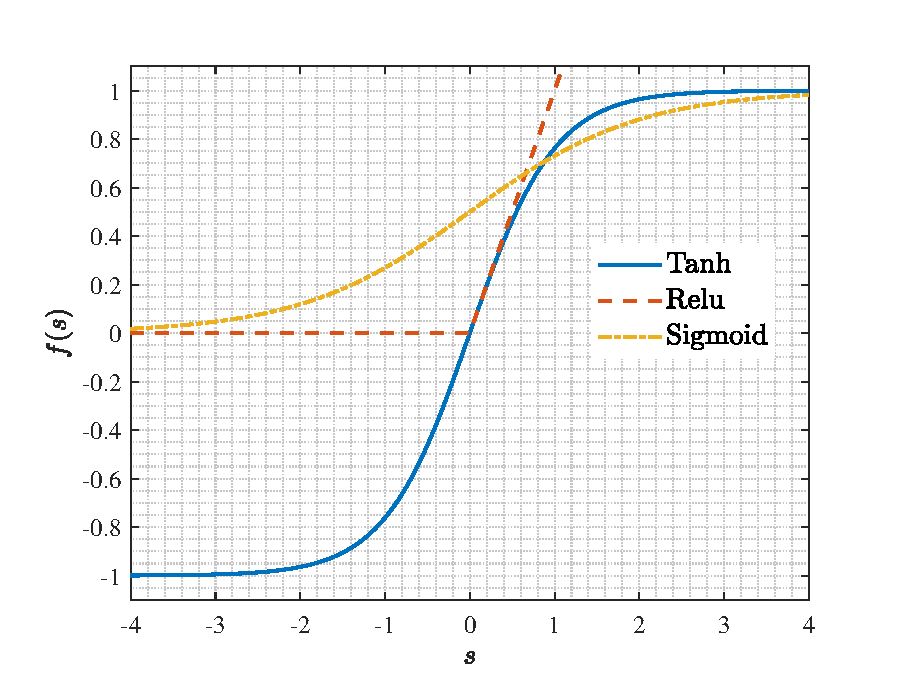
\includegraphics[width=.8\linewidth]{figures/tanh.eps}
%     \caption{Minh họa một số hàm kích hoạt được dùng trong kiến trúc đề xuất.}
%     \label{fig:tanh}
% \end{figure}

Các tham số của việc học sẽ bao gồm:
\begin{equation}
\boldsymbol{\Theta}=\left\{w^1_{k}, b^1_{k}, w^2_{k}, b^2_{k}, \alpha^1_k, \alpha^2_k \right\}_{k=1}^K
\end{equation}

Một hàm mất mát MSE cũng được định nghĩa như trên phương trình~(\ref{eq:lossdetnet}) của DetNet để biểu diễn sự hội tụ của mạng học sâu ISDNN và bước back-propagate của một mạng NN.

Bốn bước của một vòng lặp trong quá trình học như sau:
\begin{enumerate}
    \item Khởi tạo các tham số ban đầu và véc-tơ phần dư của mạng ISDNN: $\mathbf{s}_1, \mathbf{e}_1$, $\alpha^1_1, \alpha^2_1$.

    \item Bộ dữ liệu được đưa qua $K$ lớp của mạng (forward propagation), sau đó ước lượng sự mất mát qua hàm $\mathcal{L}(\mathbf{s}; \hat{\mathbf{s}}_{\boldsymbol{\Theta}}(\mathbf{H}, \mathbf{x}))$.

    \item Back-propagate $\mathcal{L}(\mathbf{s}; \hat{\mathbf{s}}_{\boldsymbol{\Theta}}(\mathbf{H}, \mathbf{x}))$ để thu được độ dốc (gradient).

    \item Từ gradient thu được, sử dụng một thuật toán tối ưu, ví dụ là Adam, cập nhật các tham số học $\boldsymbol{\Theta}=\left\{w^1_{k}, b^1_{k}, w^2_{k}, b^2_{k}, \alpha^1_k, \alpha^2_k \right\}_{k=1}^K$.
\end{enumerate}

\subsection{Đề xuất mạng nơ-ron sâu ISDNN cho mô hình kênh truyền có cấu trúc}

Khi mô hình kênh truyền dạng có cấu trúc như đã trình bày tại chương~\ref{sec:CRB}, một phần thông tin bên lề gồm DoA và cấu hình mảng ăng-ten tại bên thu được đề xuất sử dụng cho việc học của mạng ISDNN. Lý do chọn thông tin DoA là do trong các hệ mMIMO, kỹ thuật định hướng búp sóng (beamforming) có vai trò đặc biệt quan trọng trong việc tăng công suất truyền và giảm tỷ lệ tạp âm liên người dùng. Trước khi kỹ thuật beamforming có thể được sử dụng, việc biết hướng cần phát, hay hướng của người dùng (UE - User Equipment) là điều kiện cần có. Góc phát này được ước lượng thông qua tín hiệu từ các phiên truyền đường lên trước đó. Các thuật toán phổ biến được sử dụng để ước lượng hướng sóng đến như phương pháp CBF, Capon, hay MUSIC. 
\begin{equation}
    \label{eq:28}
    h_{l, t} = \beta_{l, t} e^{\varphi_{l, t}} = \beta_{l, t} e^{-i k_s c_l (\theta_{l, t}, \phi_{l, t})}
\end{equation}

Với giả thiết rằng DoA, tức các véc-tơ $\boldsymbol\theta, \boldsymbol\phi$, của các UE đã được trạm cơ sở ước lượng và khả dụng trước khi thực hiện ước lượng kênh truyền, kiến trúc ISDNN sẽ được sửa đổi để phù hợp hơn với mô hình kênh có cấu trúc như trong phương trình~(\ref{eq:28}) (gọi tắt là \textbf{ISDNN có cấu trúc}). Trước hết, thay vì phải ước lượng ma trận $\mathbf{H}$, do biết trước $\boldsymbol\theta, \boldsymbol\phi$ cũng như cấu hình của mảng ăng-ten tại trạm cơ sở, ma trận $\mathbf{H}$ được giản ước về chỉ còn thành phần hệ số khuếch đại phức của các tia ($\hat{\boldsymbol{\beta}}$). Phương trình~(\ref{eq:betahat}) biểu diễn các hệ số của ma trận kênh truyền trong trường hợp đơn giản, chỉ có tầm nhìn thẳng (LOS) hay $M = 1$.
\begin{equation}
\label{eq:betahat}
    \hat{\beta}_{l, t} = \frac{h_{l, t}} {\varphi_{l,t}}= \frac{h_{l, t}}{e^{-i k_s c_l (\theta_{l,t}, \phi_{l, t})}}
\end{equation}
Dùng phép chia vô hướng ở đây là do giả thiết các hệ số trong mô hình kênh truyền trên (\ref{eq:28}) là dạng rời rạc và vô hướng. Thực hiện tương tự với véc-tơ tín hiệu thu được $\mathbf{x}$. Giả thiết rằng, với toàn bộ thông tin véc-tơ lái $\boldsymbol{\varphi}$, véc-tơ $\mathbf{x}$ có thể được biến đổi về dạng $\hat{\mathbf{x}}$ khi kênh truyền chỉ được đại diện bởi các hệ số $\boldsymbol{\beta}$ như trên phương trình~(\ref{eq:betahat}) thông qua phép biến đổi $f_1$.
\begin{equation}
    \hat{\mathbf{x}} \longleftarrow f_1(\mathbf{x}, \boldsymbol{\varphi})
\end{equation}

Từ ma trận $\hat{\boldsymbol{\beta}}$ và véc-tơ $\hat{\mathbf{x}}$ thu được, các dữ liệu đầu vào còn lại trong mạng ISDNN cũng được thay đổi thông qua một tập các hàm xử lý tín hiệu đơn giản gọi tắt là $f_2$. Trong đó, hai giá trị $\mathbf{D}$ và $\hat{\mathbf{s}}_{1}$ có biểu diễn là:
\begin{equation}
    \begin{aligned}
        \mathbf{D} &= \operatorname{diag}(\hat{\boldsymbol{\beta}}^\top \hat{\boldsymbol{\beta}}) \\
        \hat{\mathbf{s}}_{1} &= \mathbf{D}^{-1} \hat{\boldsymbol{\beta}}^\top \hat{\mathbf{x}}
    \end{aligned}
\end{equation}

Kiến trúc một lớp mạng ISDNN cho kênh truyền có cấu trúc với thông tin bên lề là DoA tại bên thu được biểu diễn như trên hình~\ref{fig:ISD_structured}. Các tham số khởi tạo và quá trình đào tạo của mạng vẫn tương tự như kiến trúc ISDNN đã được trình bày sử dụng cho mô hình kênh truyền không sử dụng cấu trúc tại mục~\ref{sec:ISNN_nonstructured}.
\begin{figure}[ht]
    \centering
    \begin{tikzpicture}
        \node (B11) [field6, fill=red!10!white] at (0, 0) {$\mathbf{e}_k$};
        \node (B21) [below=10mm of B11, field6, fill=red!10!white] {$\hat{\mathbf{s}}_k$};

        \node (B12) [right=5mm of B11, circle, fill=blue!10!white, draw=black] {$\times$};
        \node (B13) [right=5mm of B12, circle, fill=blue!10!white, draw=black] {$+$};
        \node (B14) [right=5mm of B13, circle, fill=blue!10!white, draw=black] {$\times$};
        \node (B15) [right=5mm of B14, circle, fill=blue!10!white, draw=black] {$+$};
        \node (B16) [right=5mm of B15, circle, fill=blue!10!white, draw=black] {$\times$};
        \node (B17) [right=18mm of B16, field8, fill=green!10!white, draw=black] {$\alpha^2_k$};
        \node (B18) [right=5mm of B17, circle, fill=blue!10!white, draw=black] {$\times$};

        \node (B61) [below=4mm of B12, field8, fill=green!10!white, draw=black] {$w^1_{k}$};
        \node (B62) [below=4mm of B13, field8, fill=green!10!white, draw=black] {$b^1_{k}$};
        \node (B63) [below=4mm of B14, field8, fill=green!10!white, draw=black] {$w^2_{k}$};
        \node (B64) [below=4mm of B15, field8, fill=green!10!white, draw=black] {$b^2_{k}$};
        \node (B65) [below=4mm of B16, field8, fill=green!10!white, draw=black] {$\alpha^1_k$};

        \node (B31) [below=14mm of B64, field6, fill=red!10!white] {$\hat{\boldsymbol{\beta}}^\top \hat{\boldsymbol{\beta}}$};
        \node (B41) [below=10mm of B31, field6, fill=red!10!white] {$\hat{\boldsymbol{\beta}}^\top \hat{\mathbf{x}}$};
        \node (B51) [below=10mm of B41, field6, fill=red!10!white] {$\mathbf{D}^{-1}$};

        \node (B22) [right=75mm of B21, circle, fill=blue!10!white, draw=black] {$+$};
        \node (B23) [below=12mm of B18, circle, fill=blue!10!white, draw=black] {$+$};
        \node (B24) [right=3mm of B23, circle, fill=blue!10!white, draw=black] {$\Psi$};

        \node (B25) [below=4mm of B23, circle, fill=blue!10!white, draw=black] {$\times$};
        \node (B26) [below=4mm of B25, field8, fill=green!10!white, draw=black] {$1 - \alpha^2_k$};

        \node (B32) [right=5mm of B31, circle, fill=blue!10!white, draw=black] {$\times$};
        \node (B42) [right=5mm of B41, circle, fill=blue!10!white, draw=black] {$-$};
        \node (B52) [right=5mm of B51, circle, fill=blue!10!white, draw=black] {$\times$};

        \node (Phi1) [right=123mm of B21, field6, fill=red!10!white] {$\hat{\mathbf{s}}_{k+1}$};
        \node (V1) [right=66mm of B51, field6, fill=red!10!white] {$\mathbf{e}_{k+1}$};

        \node (H) [below=7mm of B21, field6, fill=red!10!white] {$\mathbf{H}$};
        \node (varphi) [below=10mm of H, field6, fill=red!10!white] {$\boldsymbol{\varphi}$};
        \node (x) [below=10mm of varphi, field6, fill=red!10!white] {$\mathbf{x}$};

        % \node (B71) [right=3mm of varphi, circle, fill=blue!10!white, draw=black] {$\times$};
        % \node (B72) [right=3mm of B71, circle, fill=blue!10!white, draw=black] {$+$};
        % \node (B81) [below=4mm of B71, field8, fill=green!10!white, draw=black] {$\mathbf{W}^3_{k}$};
        % \node (B82) [below=4mm of B72, field8, fill=green!10!white, draw=black] {$\mathbf{b}^3_{k}$};

        \node (B91) [below=25mm of B61 , circle, fill=blue!10!white, draw=black] {$\div$};
        \node (B92) [below=12mm of B91 , circle, fill=blue!10!white, draw=black] {$f_1$};
        \node (B93) [right=3mm of B91, field6, fill=red!10!white, minimum width=2mm, draw=black] {$\hat{\boldsymbol{\beta}}$};
        \node (B94) [right=25mm of varphi , circle, fill=blue!10!white, draw=black] {$f_2$};
        \node (B95) [right=3mm of B92, field6, fill=red!10!white, minimum width=2mm, draw=black] {$\hat{\mathbf{x}}$};

        \draw[arrow] (H) -| (B91);
        \draw[arrow] ([yshift=3mm]varphi) -| (B91);
        \draw[arrow] (x) -| (B92);
        \draw[arrow] ([yshift=-3mm]varphi) -| (B92) ;
        \draw[arrow] (B91) -- (B93);
        \draw[arrow] (B92) -- (B95);
        \draw[arrow] (B95) -| (B94);
        \draw[arrow] (B93) -| (B94);

        \draw[arrow] (B11) -- (B12);
        \draw[arrow] (B12) -- (B13);
        \draw[arrow] (B13) -- (B14);
        \draw[arrow] (B14) -- (B15);
        \draw[arrow] (B15) -- (B16);
        \draw[arrow] (B17) -- (B18);
        
        \draw[arrow] (B61) -- (B12);
        \draw[arrow] (B62) -- (B13);
        \draw[arrow] (B63) -- (B14);
        \draw[arrow] (B64) -- (B15);
        \draw[arrow] (B65) -- (B16);

        \draw[arrow] (B21) -- (B22);
        \draw[arrow] (B31) -- (B32);
        \draw[arrow] (B41) -- (B42);
        \draw[arrow] (B51) -- (B52);
        \draw[arrow] (B52) -- (V1);

        \draw[arrow] (B18) -- (B23);
        \draw[arrow] (B23) -- (B24);
        \draw[arrow] (B24) -- (Phi1);

        \draw[arrow] (B16) -| (B22);
        \draw[arrow] (B25) -- (B23);
        \draw[arrow] (B26) -- (B25);
        \draw[line] (B22) -- ([xshift=3mm]B22.east);
        \draw[arrow] ([xshift=3mm]B22.east) |- (B25);
        \draw[line] (V1) -- ([yshift=15mm]V1.north);
        \draw[arrow] ([yshift=15mm]V1.north) -| (B22);

        \draw[arrow] (B21) -| (B32);
        \draw[arrow] (B32) -- (B42);
        \draw[arrow] (B42) -- (B52);

        \draw[line] (B21) -| ([xshift=-3mm, yshift=28mm]B21.west);
        \draw[arrow] ([xshift=-3mm, yshift=28mm]B21.west) -| (B18);

        \draw[arrow] (Phi1) -- ([xshift=3mm]Phi1.east);
        \draw[arrow] (V1) -- ([xshift=3mm]V1.east);

        % \draw[arrow] (varphi) -- (B71);
        % \draw[arrow] (B71) -- (B72);
        % \draw[arrow] (B81) -- (B71);
        % \draw[arrow] (B82) -- (B72);
        % \draw[arrow] (H) -- (B91);
        % \draw[arrow] (B72) -- (B91);
        % \draw[arrow] (B91) -- (B92);
        \draw[line] (B94) -- ([xshift=3mm]B94.east);
        \draw[arrow] ([xshift=3mm]B94.east) |- (B31);
        \draw[arrow] ([xshift=3mm]B94.east) -- (B41);
        \draw[arrow] ([xshift=3mm]B94.east) |- (B51);

        % \draw[line] (x) -- ([xshift=30mm]x.east);
        % \draw[arrow] ([xshift=30mm]x.east) |- (B41);

        % Legends
        \node[rectangle, draw=black, dashed, fill=black!5!white, minimum width=140mm, minimum height=35mm] at (70mm, -105mm) {};

        \node (B51) [field6, fill=red!10!white] at (18mm, -97mm) {Giá trị \\đầu vào/đầu ra};

        \node (B61) [below=4mm of B51, field8, fill=green!10!white, draw=black] {Giá trị học};

        \node (B52) [right=7mm of B51, circle, fill=blue!10!white, draw=black] {$\times$};
        \draw[arrow] (B52) -- ([xshift=3mm]B52.east) node [pos=0, right=3mm] {Nhân};

        \node (B53) [below=7mm of B52, circle, fill=blue!10!white, draw=black] {$+$};
        \draw[arrow] (B53) -- ([xshift=3mm]B53.east) node [pos=0, right=3mm] {Cộng};

        \node (B56) [right=23mm of B52, circle, fill=blue!10!white, draw=black] {$\div$};
        \draw[arrow] (B56) -- ([xshift=3mm]B56.east) node [pos=0, right=3mm] {Chia};

        \node (B57) [below=7mm of B56, circle, fill=blue!10!white, draw=black] {$-$};
        \draw[arrow] (B57) -- ([xshift=3mm]B57.east) node [pos=0, right=3mm] {Trừ};

        \node (B54) [right=55mm of B52, circle, fill=blue!10!white, draw=black] {$\Psi$};
        \draw[arrow] (B54) -- ([xshift=10mm]B54.east) node [pos=0, right=11mm, above, label={below}:{phi tuyến tính}] {Toán tử};

        \node (B55) [right=55mm of B53, circle, fill=blue!10!white, draw=black] {$f$};
        \draw[arrow] (B55) -- ([xshift=3mm]B55.east) node [pos=0, right=11mm, above, label={below}:{lý dữ liệu}] {Các hàm xử};
    \end{tikzpicture}
    \caption{Kiến trúc của một lớp trong mạng nơ-ron sâu ISDNN đề xuất cho mô hình kênh truyền có cấu trúc. Giả sử biết thông tin của DoA và cấu hình mảng ăng-ten tại bên thu $\boldsymbol{\varphi}(\boldsymbol\theta, \boldsymbol\phi$).}
    \label{fig:ISD_structured}
\end{figure}

\section{Mô phỏng và đánh giá}

\subsection{Tạo bộ dữ liệu}

\begin{table}[ht]
    \centering
    \caption{Các tham số mô phỏng hệ thống truyền thông không dây của mạng nơ-ron sâu ISDNN được đề xuất.}
    \label{tab:simu_param}
    \begin{tabular}{p{8cm}|p{6cm}} 
    \hline
    \hline
    \multicolumn{1}{c|}{\textbf{Thông số mô phỏng}} & \multicolumn{1}{c} {\textbf{Giá trị}} \\ 
    \hline
    Kích thước hệ thống mMIMO & $T = 8, L =64$ \\ 
    \hline
    Loại điều chế & $16$-QAM\\
    \hline
    Các mức $\operatorname{SNR}$ của bộ dữ liệu  & $[0, 5, 10, 15, 20]$~dB \\ 
    \hline
    Số mẫu đào tạo & $20.000$ \\ 
    \hline
    Số mẫu thử nghiệm & $5.000$ \\ 
    \hline
    Số lớp mạng của DetNet & $K_{DetNet} = 4; 10$\\ 
    \hline
    Số lớp mạng của ISDNN & $K_{ISDNN} = 4$ \\ 
    \hline
    Số lượng mẫu trong một lần huấn luyện & Batch size $= 20.000$ \\ 
    \hline
    Thuật toán tối ưu & Adam~ \\ 
    \hline
    Giá trị khởi tạo của tốc độ học & $\delta = 0$,$0001$ \\ 
    \hline
    Số vòng lặp đào tạo & $20.000$ \\
    \hline
    \end{tabular}
\end{table}
Trong bảng~\ref{tab:simu_param}, các tham số mô phỏng của hệ thống mMIMO cũng như kiến trúc mạng DetNet và ISDNN được đưa ra. 
% Chi tiết, các tập dữ liệu được tạo cho việc huấn luyện (training)/thử nghiệm (testing) sẽ độc lập với nhau nhưng cùng chung phân bố. Mỗi tín hiệu của bên phát $\mathbf{s}$ sẽ được gieo ngẫu nhiên theo phân bố đều và sử dụng chung một loại điều chế. 
% Tuy nhiên thay vì gieo trực tiếp các ký hiệu như mô phỏng của SB-MRE là các nhóm bít $\{0 , 1\}$.
% Tuỳ thuộc vào loại điều chế, mà một nhóm gồm $1, 2, 4, 8,~\ldots$ bít sẽ được nhóm thành một ký hiệu. Trong mô phỏng, điều chế $16$-QAM được lựa chọn, với $4$ bít liền nhau sẽ được gộp lại, $\mathbf{u}_i \in \mathbb{R}^4$, tạo thành ký hiệu $s_i$. Trên bảng~\ref{tab:mapping}
% và hình~\ref{fig:mapping}
% là quy luật ánh xạ các nhóm $4$ bít thành các ký hiệu $s_i$.
% \begin{table}[ht]
% \centering
% \caption{Ánh xạ các nhóm $4$ bít thành các ký hiệu sử dụng điều chế $16$-QAM.}
% \label{tab:mapping}
% \resizebox{\textwidth}{!}{
%     \begin{tabular}{|l|l|l|l|l|} 
%     \hline
%     \multirow{4}{*}{\begin{tabular}[c]{@{}l@{}}\textbf{Ký}\\ \textbf{hiệu}\end{tabular}}
%     & $s_0 = -1 -1i$ & $s_1 = -1 -0,33i$& $s_2 = -1 +0,33i$  & $s_3 = -1 +1i$ \\
%     \cline{2-5}
%     & $s_4 = -0,33 -1i$  & $s_5 = -0,33 -0,33i$ & $s_6 = -0,33 +0,33i$ &  $s_7 = -0,33 +1i$ \\
%     \cline{2-5}
%     & $s_8 = 0,33 -1i$ & $s_9 = 0,33 -0,33i$ & $s_{10} = 0,33 +0,33i$ & $s_{11} = 0,33 +1i$ \\
%     \cline{2-5}
%     & $s_{12} = 1 -1i$ & $s_{13} = 1 -0,33i$ & $s_{14} = 1 +0,33i$ & $s_{15} = 1 +1i$ \\
%     \hline
%     \multirow{4}{*}{\begin{tabular}[c]{@{}l@{}}\textbf{Nhóm}\\ \textbf{bít}\end{tabular}}
%     & $\mathbf{u}_0 = [0, 0, 0, 0]$ & $\mathbf{u}_1 = [0, 0, 0, 1]$ 
%     & $\mathbf{u}_2 = [0, 0, 1, 0]$ & $\mathbf{u}_3 = [0, 0, 1, 1]$ \\ \cline{2-5}
    
%     & $\mathbf{u}_4 = [0, 1, 0, 0]$ & $\mathbf{u}_5 = [0, 1, 0, 1]$ 
%     & $\mathbf{u}_6 = [0, 1, 1, 0]$ & $\mathbf{u}_7 = [0, 1, 1, 1]$ \\
%     \cline{2-5}
    
%     & $\mathbf{u}_8 = [1, 0, 0, 0]$ & $\mathbf{u}_9 = [1, 0, 0, 1]$ 
%     & $\mathbf{u}_{10} = [1, 0, 1, 0]$ & $\mathbf{u}_{11} = [1, 0, 1, 1]$ \\
%     \cline{2-5}
    
%     & $\mathbf{u}_{12} = [1, 1, 0, 0]$ & $\mathbf{u}_{13} = [1, 1, 0, 1]$ 
%     & $\mathbf{u}_{14} = [1, 1, 1, 0]$ & $\mathbf{u}_{15} = [1, 1, 1, 1]$ \\
%     \hline
%     \end{tabular}
% }
% \end{table}
% \begin{figure}[ht]
%     \centering
%     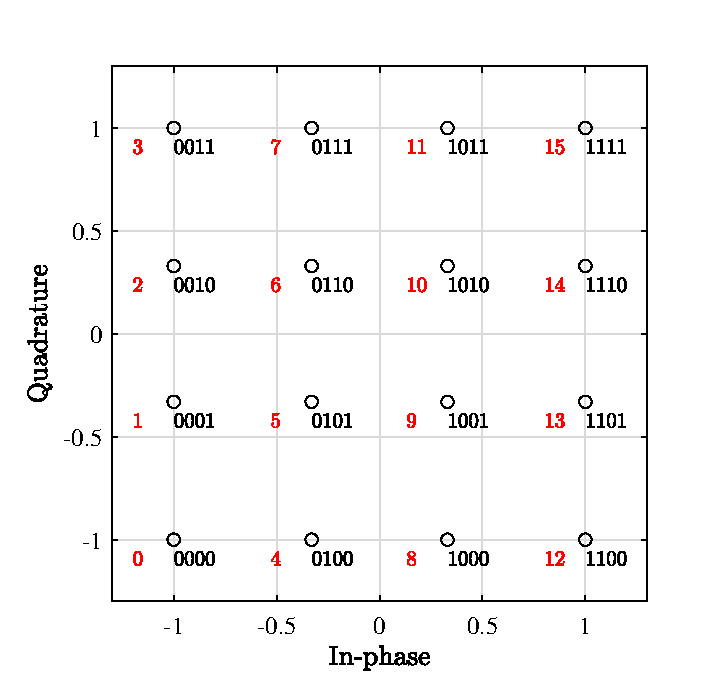
\includegraphics[width=.8\linewidth]{figures/qam16_con.eps}
%     \caption{Ánh xạ các nhóm $4$ bít thành các ký hiệu sử dụng điều chế $16$-QAM.}
%     \label{fig:mapping}
% \end{figure}

% Ma trận kênh truyền $\mathbf{H}$ lấy theo mô hình kênh CBSM i.i.d Rayleigh đã trình bày trong chương~\ref{sec:back}, trong đó, các hệ số phức của kênh truyền được gieo ngẫu nhiên độc lập và cùng phân bố Gauss với giá trị trung bình $\mu$ và phương sai $\sigma^2$ như trên hình~\ref{fig:ray_H}.
% \begin{equation}
% \Re(h_{l, t})=f(x \mid \mu, \sigma)=\frac{1}{\sigma \sqrt{2 \pi}} e^{\frac{-(x-\mu)^2}{2 \sigma^2}}, \quad \text { với } x \in \mathbb{R}
% \end{equation}
% \begin{figure}
%     \centering
%     \begin{subfigure}{.48\linewidth}
%         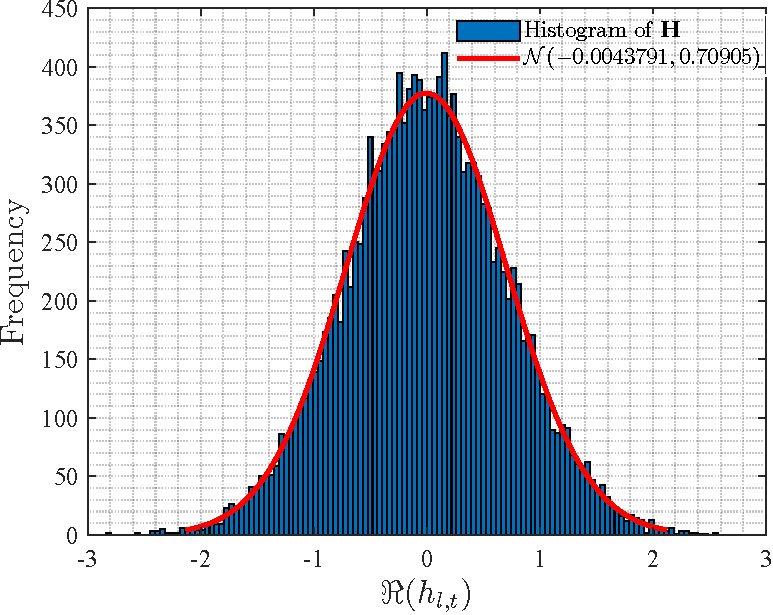
\includegraphics[width=\linewidth]{figures/H.pdf}
%         \caption{$\mathbf{H}$}
%         \label{fig:ray_H}
%     \end{subfigure}
%     \hfill
%     \begin{subfigure}{.48\linewidth}
%         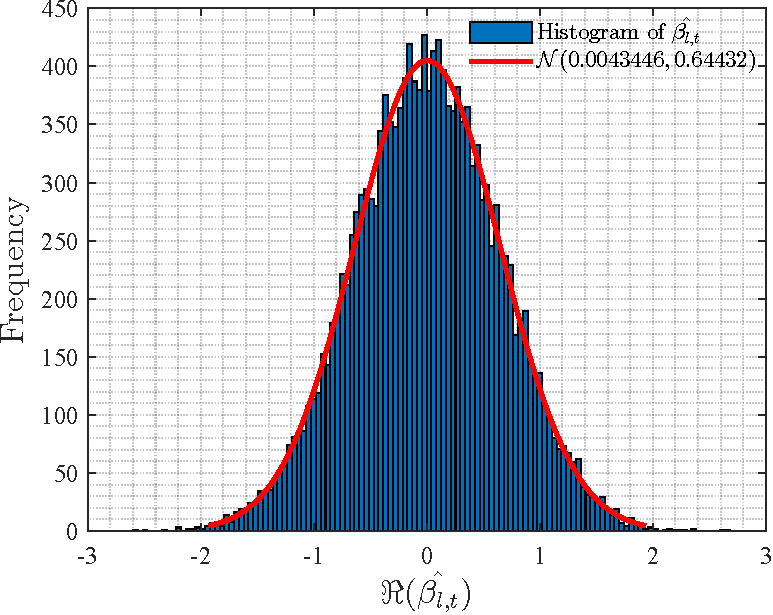
\includegraphics[width=\linewidth]{figures/Beta.pdf}
%         \caption{$\hat{\boldsymbol{\beta}}$}
%         \label{fig:ray_Beta}
%     \end{subfigure}
%     \caption{Phân bố khi gieo ngẫu nhiên của các hệ số phần thực của $h_{l, t}$ và $ \hat{\beta}_{l, t}$ trong hai ma trận $\mathbf{H}$, $\hat{\boldsymbol{\beta}}$.}
%     \label{fig:ray}
% \end{figure}

% Trong mô hình kênh truyền có cấu trúc, vẫn giữ nguyên cách gieo ngẫu nhiên như ma trận $\mathbf{H}$ như mô hình không sử dụng cấu trúc. Sau đó, từ các thông tin bên lề là DoA và cấu hình mảng ăng-ten thu, các giá trị thuộc ma trận $\hat{\boldsymbol{\beta}}$ được tính ngược lại theo công thức~(\ref{eq:betahat}). Trên hình~\ref{fig:ray_Beta} là biểu diễn histogram các giá trị phần thực $\hat{\beta}_{l, t}$ thuộc ma trận $\hat{\boldsymbol{\beta}}$. Có thể nhận thấy các phần tử trong ma trận $\mathbf{H}$ và $\hat{\boldsymbol{\beta}}$ cùng có phân bố chuẩn với kỳ vọng xấp xỉ bằng $0$. Sự khác nhau nằm ở phương sai của các phân bố này, lần lượt là $\approx \mathcal{N} (0; \frac{1}{\sqrt{2}})$, $\mathcal{N} (0; 0,644)$ ứng với $\Re(h_{l, t})$ và $\Re(\hat{\beta}_{l, t})$. Với phương sai nhỏ hơn, có thể dự đoán rằng các mạng học sâu như ISDNN có cấu trúc có thể cho ra các hệ số của ma trận $\hat{\boldsymbol{\beta}}$ nhanh và chính xác hơn không sử dụng cấu trúc $\mathbf{H}$.
% . Sự khác nhau nằm ở cách sắp xếp các giá trị ngẫu nhiên này để tạo thành hai ma trận kể trên, điều này sẽ dẫn đến các kết quả học khác nhau trong quá trình đào tạo.

% Ngoài việc đào tạo dựa trên các thông tin kênh truyền $\mathbf{H}$ và $\hat{\boldsymbol{\beta}}$ chính xác. Trước hết, xem xét việc đào tạo ISDNN cho mô hình kênh không sử dụng cấu trúc trong trường hợp thông tin $\mathbf{H}$ không chính xác (im - imperfect) để kiểm tra khả năng chịu lỗi của kiến trúc mạng nơ-rơn sâu ISDNN đề xuất. Lý do là trong các điều kiện thực tế, các ma trận đầu vào để đào tạo được đo lường không thể có được sự chính xác hoàn hảo. Hai mức sai số sẽ được xem xét đó là $1\%$ và $5\%$.
% \begin{equation}
% \begin{aligned}
%      \mathbf{H}_{im} &= \mathbf{H} \pm 0,01\mathbf{H} \\
%      \mathbf{H}_{im} &= \mathbf{H} \pm 0,05\mathbf{H}
% \end{aligned}
% \end{equation}
% Tương tự, xem xét việc đào tạo kiến trúc mạng ISDNN cho mô hình kênh có cấu trúc trong trường hợp cả thông tin $\mathbf{H}$ và ${\boldsymbol{\varphi}}$ đều có sai số. Sai số từ $\mathbf{H}$ vẫn tương tự như giả thiết của mô hình kênh không sử dụng cấu trúc. Sai số của dữ liệu đầu vào ${\boldsymbol{\varphi}}$ đến từ việc ước lượng sai các giá trị $(\boldsymbol{\theta}, \boldsymbol{\phi})$. Tương tự như trên, hai mức sai số của ${\boldsymbol{\varphi}}$ sẽ được xem xét đó là $1\%$ và $5\%$. Sai số của ${\boldsymbol{\varphi}}$ được gọi là ``\textbf{sai số của thông tin bên lề}''.
% \begin{equation}
%     \begin{aligned}
%          {\boldsymbol{\varphi}}_{im} &= {\boldsymbol{\varphi}} \pm 0,01{\boldsymbol{\varphi}} \\
%          {\boldsymbol{\varphi}}_{im} &= {\boldsymbol{\varphi}} \pm 0,05{\boldsymbol{\varphi}}
%     \end{aligned}
% \end{equation}

Sau khi đi qua kênh truyền $\mathbf{H}$, các ký hiệu sẽ được cộng thêm với AWGN ở các giá trị $\operatorname{SNR}$ khác nhau tính theo thang dB (decibel). 
\begin{equation}
\operatorname{SNR} = 10 \log \left(\frac{\mathbb{E}\left(\|\mathbf{H s}\|_2^2\right)}{\mathbb{E}\left(\|\mathbf{w}\|_2^2\right)}\right)~\text{(dB)}
\end{equation}
Cụ thể, trong bộ dữ liệu đào tạo, $5$ ngưỡng $\operatorname{SNR}$ khác nhau, lần lượt là $0, 5, 10, 15,$ và~$20$~dB được thêm vào các mẫu huấn luyện, sau đó bộ dữ liệu này được trộn ngẫu nhiên.

\subsection{Đào tạo và đánh giá kiến trúc mạng nơ-ron sâu đề xuất}

\subsubsection*{\textbf{Phương pháp đánh giá}}

% Sau khi đã tạo được các bộ dữ liệu, việc đào tạo được triển khai trên máy tính với cấu hình: vi xử lý Intel Core i9-10900, 64~GB RAM. Ngôn ngữ lập trình Python được lựa chọn để xây dựng các mô phỏng của ISDNN và DetNet. 
Thư viện nền tảng Pytorch được sử dụng cho ISDNN, và Tensorflow cho DetNet. Mã nguồn của DetNet lấy từ kho lưu trữ công khai của nhóm tác giả trên bài báo gốc tại Github\footnote{\url{https://github.com/neevsamuel/DeepMIMODetection}}. Sai số của các mạng nơ-ron này được đánh giá thông qua thông số BER tương ứng là số bít ước lượng sai ($N_e$) chia cho tổng số bít. Ở bước thử nghiệm, $100$ bộ dữ liệu thử nghiệm, mỗi bộ gồm $5.000$ mẫu được tạo ra, kết quả ước lượng của các mô hình thu được sau quá trình đào tạo được tính bằng BER trung bình của $100$ lần thử nghiệm.
\begin{equation}
    \operatorname{BER} = \frac{1}{100} \sum_{K=1}^{100} \frac{N_e}{5000}
\end{equation}

\subsubsection*{\textbf{So sánh độ phức tạp của các phương pháp}}
Độ phức tạp của các thuật toán sẽ được so sánh như trên bảng~\ref{tab:computational}. Trong đó, hai bộ nhận dạng truyền thống ZF và MMSE đều có độ phức tạp $\mathcal{O}(TL^3)$ do phép nghịch đảo của ma trận $\mathbf{H}$ với kích thước đầy đủ. Tiếp đến, kiến trúc mạng DetNet cho độ phức tạp $\mathcal{O}(TL^2)$ do không phải nghịch đảo ma trận $\mathbf{G}_\mathbf{H}$ nên thành phần phức tạp nhất trong DetNet là các phép nhân ma trận $\mathbf{H}^\top \mathbf{H}$ và $\mathbf{H}^\top \mathbf{H} \hat{\mathbf{s}}_k$. Cuối cùng là độ phức tạp của kiến trúc mạng ISDNN được đề xuất cho cả hai mô hình kênh truyền có cấu trúc và không sử dụng cấu trúc cũng ở mức $\mathcal{O}(TL^2)$. Dù có phép nghịch đảo ma trận $\mathbf{D}^{-1}$ ở đầu vào, tuy nhiên như đã trình bày ở trên, ma trận $\mathbf{D}$ chỉ gồm các phần tử trên đường chéo chính của ma trận Gram. Do vậy, việc nghịch đảo ma trận này chỉ có độ phức tạp $\mathcal{O}(TL)$, vì chỉ cần sử dụng phép biến đổi tuyến tính. Vậy nên, độ phức tạp tổng thể của ISDNN vẫn tương tự như DetNet chỉ dừng ở các phép nhân ma trận. Có thể kết luận rằng, các phương pháp sử dụng học sâu đã giảm thiểu độ phức tạp đi $\mathcal{O}(L)$ so với các bộ ước lượng tuyến tính truyền thống. Đây là khoảng cách rất lớn, vì trong các hệ mMIMO, giá trị của $L$ có thể lên đến hàng nghìn. So sánh riêng hai kiến trúc mạng DNN là DetNet và ISDNN, dù có chung độ phức tạp nhưng nhận thấy số lượng giá trị học của ISDNN là không đáng kể khi so sánh với DetNet. Điều này có được là do các bộ biến đổi tuyến tính ($\mathbf{W}, \mathbf{b}$) trong DetNet ở dưới dạng ma trận và véc-tơ có kích thước lớn. Trong khi đó, ISDNN chỉ yêu cầu hai tham số học vô hướng ($w, b$) cho mỗi bộ biến đổi tại mỗi lớp mạng. Do vậy, chỉ $24$ tham số học cần được sử dụng trong ISDNN, dẫn đến mô hình thu được sau quá trình đào tạo chỉ có kích thước $7$~KB so với $1,236$~KB của DetNet với cùng số lớp mạng là $4$. Đây là lợi thế rất lớn, khi kích thước nhỏ và độ phức tạp thấp giúp làm tăng khả năng ứng dụng trên cả các thiết bị có giá thành thấp.
\begin{table}[t]
    \centering
    \caption{So sánh độ phức tạp của các thuật toán nhận dạng kênh truyền.}
    \label{tab:computational}
    \begin{tabular}{l|c|c}
    \hline
    \hline
    \multicolumn{1}{c|}{\textbf{Bộ nhận dạng}} & \textbf{Độ phức tạp} & \textbf{Số giá trị học} \\ \hline
    ZF & $\mathcal{O}$ ($TL^3$) &  \\ \hline
    MMSE & $\mathcal{O}$ ($TL^3$) &  \\ \hline
    DetNet: 4 layers & $\mathcal{O}$ ($TL^2$) & 105.416 \\ \hline
    ISDNN unstructured& $\mathcal{O}$ ($TL^2$) & 24 \\ \hline
    ISDNN structured& $\mathcal{O}$ ($TL^2$) & 24 \\ \hline
    \end{tabular}
\end{table}

\subsubsection*{\textbf{So sánh độ chính xác của mạng nơ-ron sâu đề xuất với các phương pháp khác}}
% Trên hình~\ref{fig:training_1} là quá trình đào tạo của hai mạng nơ-ron sâu ISDNN và DetNet với số lớp mạng, mô hình kênh khác nhau. Hình~\ref{fig:loss_1} xem xét về thời gian hội tụ thông qua đầu ra của hàm mất mát giữa véc-tơ ký hiệu gốc $\mathbf{s}$ và véc-tơ ký hiệu ước lượng $\mathbf{\hat{s}}$. Nhận thấy, thời gian hội tụ của mạng DetNet với $4$ lớp mạng có phần nhanh hơn so với ISDNN có cấu trúc và không sử dụng cấu trúc cùng số lớp mạng. Tuy nhiên, xét về tổng thể, đầu ra hàm mất mát của ISDNN cả có cấu trúc và không sử dụng cấu trúc cho kết quả tốt hơn so với DetNet cùng số lớp mạng dù phải cần đến vòng đào tạo thứ $12.000$. Xét riêng hai mô hình có cấu trúc và không sử dụng cấu trúc của ISDNN, tốc độ hội tụ và giá trị của hàm mất mát tại vòng lặp cuối cùng khá tương đồng nhau khoảng $4 * 10^{-3}$. Nếu tăng số lớp mạng của DetNet lên $10$, do số lượng tham số học tăng lên đáng kể, thời gian hội tụ và đầu ra mất mát cuối cùng cũng cho kết quả tốt hơn ISDNN chỉ $4$ lớp mạng. Tuy nhiên, đánh đổi ở đây là số lượng tham số học sẽ lên đến $316.244$. Xét về sự hội tụ dựa trên tỷ lệ sai số bít của các kiến trúc như trên hình~\ref{fig:ber_1}. Trước hết, BER của ISDNN chỉ với $4$ lớp mạng sau $20.000$ vòng đào tạo là vượt trội so với DetNet dù $4$ hay $10$ lớp mạng, hội tụ ở giá trị $\operatorname{BER}\approx 4 * 10^{-4}$ và $6*10^{-4}$ lần lượt với mô hình có cấu trúc và không sử dụng cấu trúc. So sánh với DetNet dù với $10$ lớp mạng và lượng tham số học khổng lồ cũng chỉ có đạt được sai số chưa đến $10^{-3}$. Tuy nhiên, từ mô phỏng cũng cho thấy rằng, độ chính xác của DetNet cho thời gian hội tụ là nhanh hơn nhiều so với ISDNN khi chỉ cần đến khoảng $5.000$ vòng đào tạo. Trong quá trình đào tạo, thông qua cả hai thông số BER và hàm mất mát, có thể rút ra nhận xét rằng, kiến trúc ISDNN có cấu trúc cho độ chính xác trong quá trình học là tốt hơn ISDNN không sử dụng cấu trúc và DetNet, tuy nhiên, DetNet lại là mạng có thời gian hội tụ nhanh nhất.
% Với ISDNN có cấu trúc, thời gian đạt đến $\operatorname{BER}\approx 10^{-3}$ là nhanh nhất trong cả $4$ mô hình được xem xét chỉ chưa đến $5.000$ vòng đào tạo. Tuy nhiên sau đó, tương tự như hàm mất mát, giá trị BER của ISDNN có cấu trúc thay đổi liên tục trong khoảng $[10^{-2} \;\; 10^{-3}]$ không theo quy luật nào. Điều này có thể là do hai nguyên nhân: (i), số lượng tham số học của mạng nhỏ, không đủ để học ra giá trị tối ưu ứng với toàn bộ tập dữ liệu huấn luyện; (ii), tập đầu vào $\hat{\mathbf{x}}$ ước lượng được có sai số.

% \begin{figure}[t]
%      \centering
%      \begin{subfigure}[b]{0.48\textwidth}
%          \centering
%          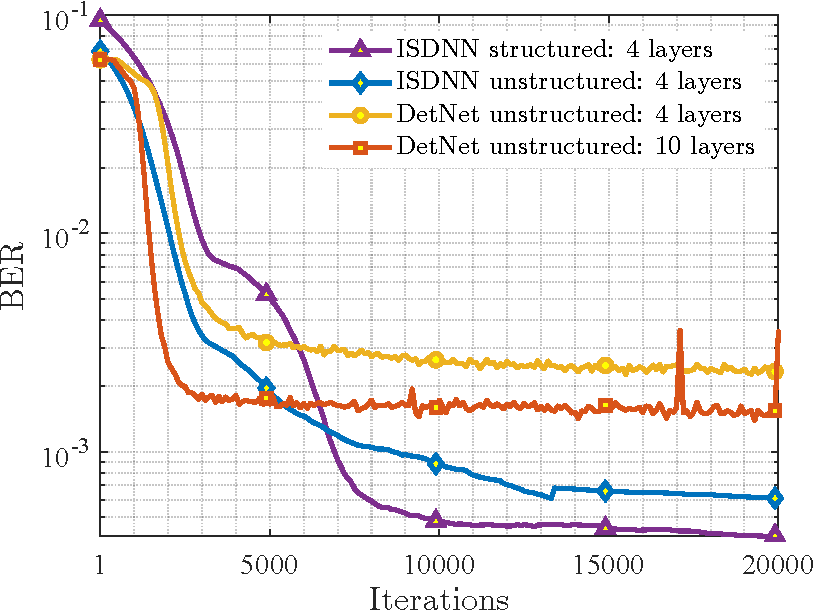
\includegraphics[width=\textwidth]{figures/BER_1.pdf}
%          \caption{BER}
%          \label{fig:ber_1}
%      \end{subfigure}
%      \hfill
%      \begin{subfigure}[b]{0.48\textwidth}
%          \centering
%          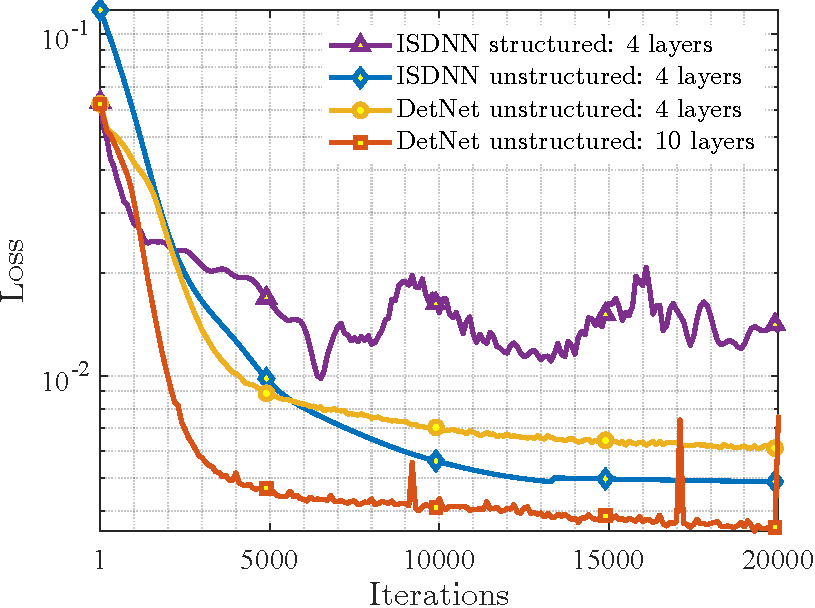
\includegraphics[width=\textwidth]{figures/Loss_1.pdf}
%          \caption{Mất mát}
%          \label{fig:loss_1}
%      \end{subfigure}
%      \hfill
%         \caption{Sự hội tụ của quá trình đào tạo mạng ISDNN và DetNet.}
%         \label{fig:training_1}
% \end{figure}
\begin{figure}[t]
    \centering
    \begin{subfigure}{\linewidth}
        \centering
        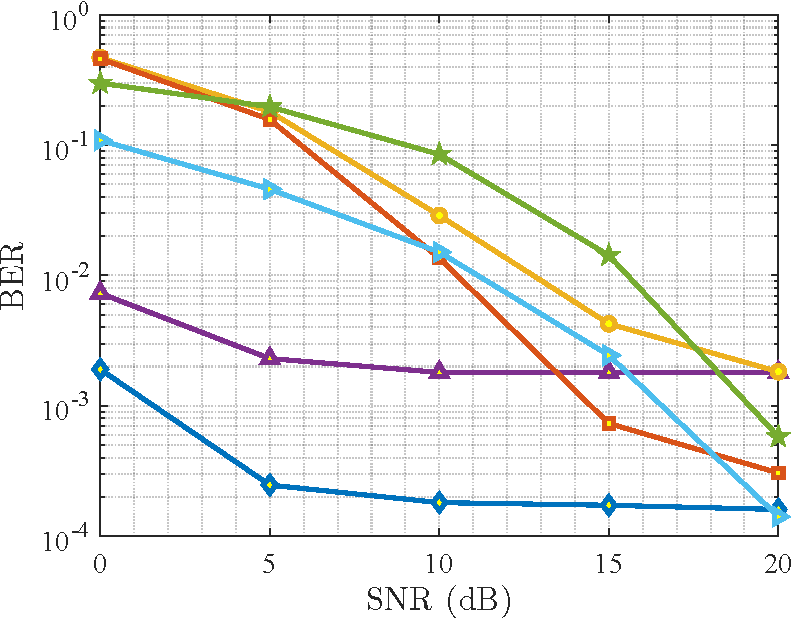
\includegraphics[width=.6\linewidth]{figures/performance_1.pdf}
    \end{subfigure}
    \hfill
    \begin{subfigure}{\linewidth}
        \centering
        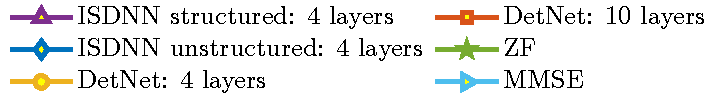
\includegraphics[width=.5\linewidth]{figures/lg_performance_1.pdf}
    \end{subfigure}
    \caption{Độ chính xác của mạng ISDNN so sánh với DetNet và các bộ nhận dạng tuyến tính.}
    \label{fig:isdnn}
\end{figure}

% Sau quá trình đào tạo, kiểm tra mô hình thu được trên các bộ dữ liệu thử nghiệm độc lập với tập dữ liệu huấn luyện. 
Kết quả thu được khi so sánh độ chính xác của các phương pháp nhận dạng kênh truyền gồm ZF, MMSE, DetNet, và ISDNN khi SNR thay đổi được biểu diễn trên hình~\ref{fig:isdnn}. 
% Trước hết, có thể kết luận, độ chính xác của mạng ISDNN đề xuất là vượt trội so với các phương pháp còn lại. Khi so sánh với hai phương pháp tuyến tính là ZF và MMSE, đường BER của ISDNN và DetNet đều cho thấy sự khác biệt, khi độ dốc của BER từ các mạng DNN giảm dần theo SNR còn ZF và MMSE thì ngược lại. Phải cần đến mức $\operatorname{SNR}=20$~dB, phương pháp MMSE mới đạt đến độ chính xác của ISDNN không sử dụng cấu trúc tức $\operatorname{BER}\approx 1,5* 10^{-4}$, do giải thuật gốc ISD cũng xuất phát từ MMSE nên có thể coi đây là giá trị tối ưu của ISD. Khi so sánh với mạng nơ-ron sâu DetNet gồm $4$ lớp mạng, ISDNN không sử dụng cấu trúc cho độ lợi về BER đạt $10^2$ tại các mức SNR thấp, và $10^1$ tại SNR cao. ISDNN có cấu trúc cho tỷ lệ sai số bít thấp hơn mạng không sử dụng cấu trúc, tuy nhiên độ lợi là chưa thực sự vượt trội, ở $\operatorname{SNR}=20$~dB, tỷ lệ lỗi bít đạt $\approx 10^{-4}$. Khi tăng số lớp của DetNet lên $10$, cũng tương tự như quá trình huấn luyện, độ chính xác đã được cải thiện, tuy nhiên dù SNR ở mức cao như $20$~dB, BER của DetNet cũng chỉ tiệm cận được đến độ chính xác của ISDNN không sử dụng cấu trúc với $4$ lớp mạng.
Có thể rút ra nhận xét, kiến trúc ISDNN ngoài việc cho độ chính xác vượt trội so với ZF, MMSE, và DetNet còn có ưu điểm là BER không có sự biến đổi quá lớn ở các mức SNR khác nhau. Đây là ưu điểm quan trọng của việc sử dụng DNN cho việc nhận dạng kênh truyền, khi tạp âm/công suất phát luôn là một vấn đề mà các thế hệ mạng viễn thông thế hệ mới như 5G quan tâm. Nếu độ chính xác của việc nhận dạng không bị phụ thuộc nhiều vào SNR thì mật độ bao phủ, cũng như hiệu quả về năng lượng là những lợi ích có thể khai thác.

\subsubsection*{\textbf{Xem xét độ chính xác của mạng nơ-ron sâu ISDNN khi có sai số trong tập dữ liệu đào tạo}}
% Tiếp theo, xem xét đến tính chống chịu lỗi của mạng nơ-ron sâu ISDNN. Như đã trình bày ở trên, để có thể được áp dụng thực tế, các bộ dữ liệu cần được thu thập từ các hệ thống viễn thông thực. Tuy nhiên, sai số khi đo lường các đầu vào cho việc đào tạo là không thể tránh khỏi. 
Trong phần này: (i), ma trận kênh truyền $\mathbf{H}$ được giả sử là có sự sai khác $1$\% và $5$\% so với $\mathbf{H}$ hoàn hảo; (ii), cả ma trận kênh truyền $\mathbf{H}$ và ma trận thông tin bên lề ${\boldsymbol{\varphi}}$ đều có sai số là $1$\% và $5$\% so với giá trị thực tế. 
% \begin{figure}[ht]
%     \centering
%     \begin{subfigure}[b]{0.48\textwidth}
%         \centering
%         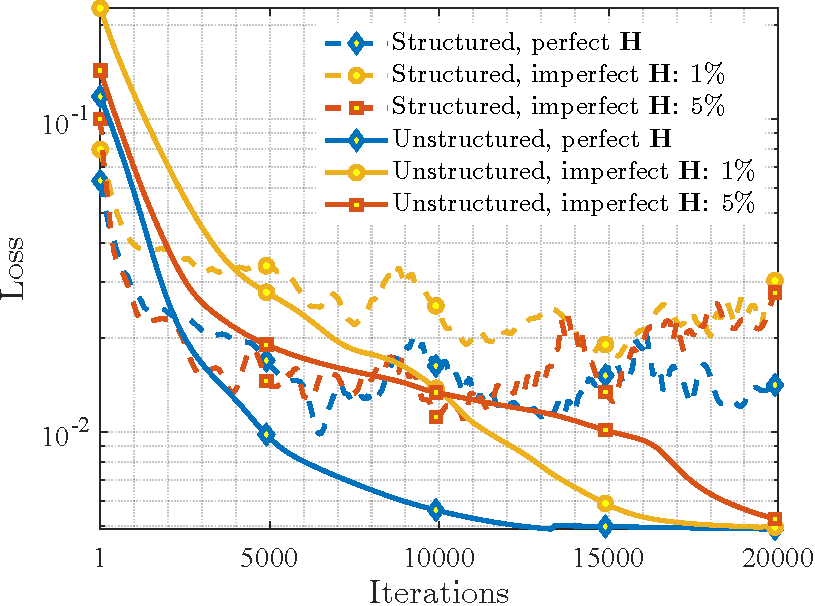
\includegraphics[width=\textwidth]{figures/BER_2.pdf}
%         \caption{BER}
%         \label{fig:ber_2}
%     \end{subfigure}
%     \hfill
%     \begin{subfigure}[b]{0.48\textwidth}
%         \centering
%         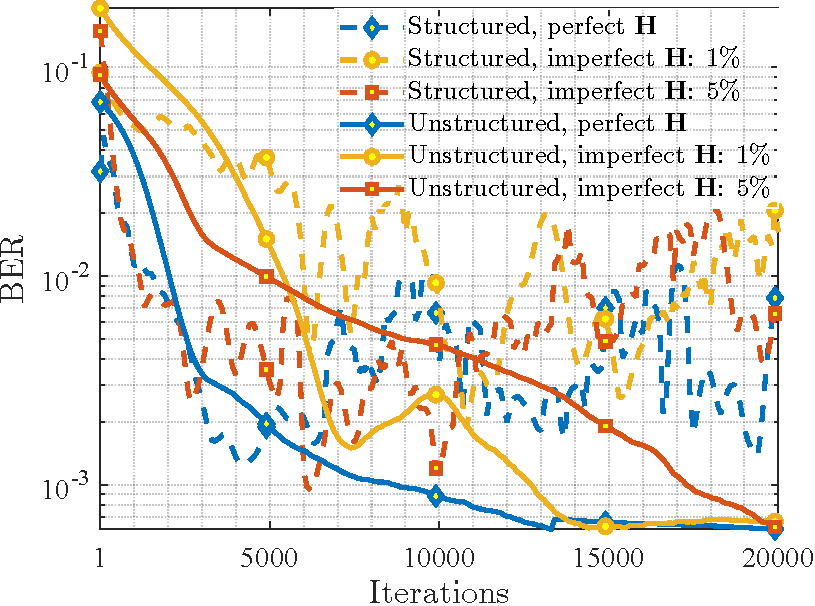
\includegraphics[width=\textwidth]{figures/Loss_2.pdf}
%         \caption{Mất mát}
%         \label{fig:loss_2}
%     \end{subfigure}
%     \hfill
%     \begin{subfigure}{\linewidth}
%         \centering
%         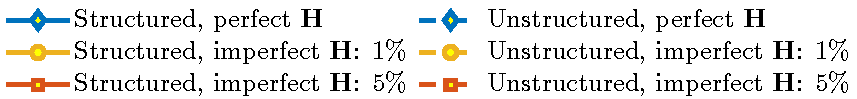
\includegraphics[width=.8\linewidth]{figures/lg_performance_21.pdf}
%     \end{subfigure}
%     \caption{Sự hội tụ của quá trình đào tạo các mạng ISDNN với các sai số kênh truyền đầu vào khác nhau.}
%     \label{fig:training_2}
% \end{figure}

% Trên hình~\ref{fig:training_2} là kết quả của việc đào tạo mạng ISDNN có cấu trúc và không sử dụng cấu trúc với $3$ bộ dữ liệu có các mức sai số kênh truyền khác nhau. Đầu tiên, hình~\ref{fig:loss_2} cho thấy rõ ràng sai số của dữ liệu đầu vào ảnh hưởng trực tiếp đến sự hội tụ của một mạng DNN. 
% Cả hai kiến trúc ISDNN với kênh truyền chính xác cho tốc độ hội tụ về hàm mất mát là nhanh hơn đáng kể khi so với trường hợp kênh truyền có sai số. Với sai số $1$\% cần đến $14.000$ và $18.000$ vòng đào tạo lần lượt với mạng có cấu trúc và không sử dụng cấu trúc để đầu ra của hàm mất mát hội tụ. Tương tự, khi sai số là $5$\%, sau $20.000$ vòng đào tạo vẫn chưa có được sự hội tụ của hàm mất mát. Tuy có sự khác nhau về tốc độ, nhưng giá trị cuối cùng của hàm mất mát tại cả $6$ trường hợp đều khá tương đồng khoảng $5*10^{-3}$.
% Tiếp theo, về độ chính xác trong quá trình đào tạo cũng cho kết quả tương đồng, biểu diễn trên hình~\ref{fig:ber_2}. Khi dữ liệu kênh truyền có sai số, đường BER trong quá trình học của các mạng ISDNN có sự không ổn định và cần đến thêm ít nhất $5.000$ vòng đào tạo để đạt được giá trị hội tụ. 
% Do đó, xét cả hàm mất mát và BER, kiến trúc ISDNN vẫn có thể thích nghi với sai số $1$\% của ma trận kênh truyền dù ảnh hưởng đến thời gian huấn luyện cần để hội tụ nhưng vẫn sẽ hội tụ ở giá trị khá tương đương với kênh truyền hoàn hảo. 
\begin{figure}[H]
    \centering
    \begin{subfigure}{\linewidth}
        \centering
        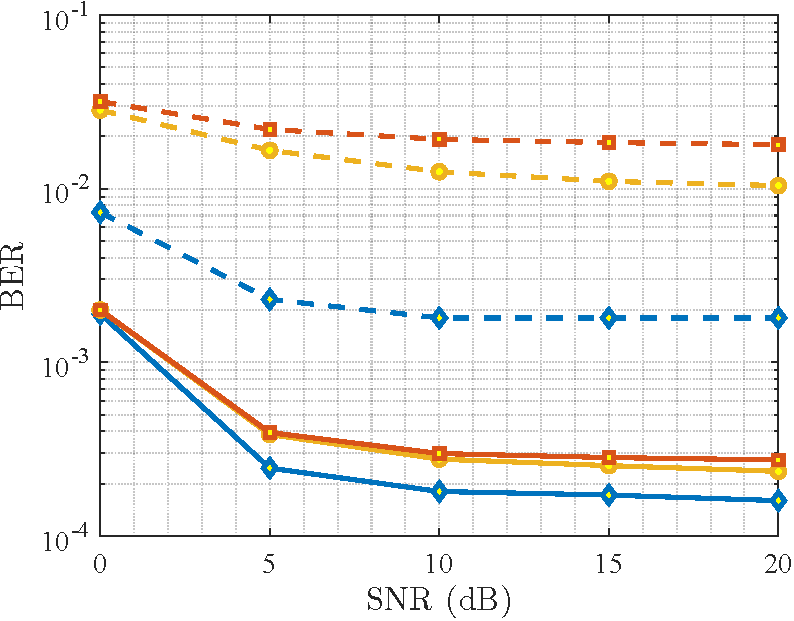
\includegraphics[width=.6\linewidth]{figures/performance_2.pdf}
    \end{subfigure}
    \hfill
    \begin{subfigure}{\linewidth}
        \centering
        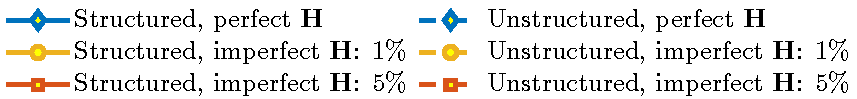
\includegraphics[width=.6\linewidth]{figures/lg_performance_21.pdf}
    \end{subfigure}
    \caption{Độ chính xác của mạng ISDNN với các sai số kênh truyền đầu vào khác nhau.}
    \label{fig:isdnn_1}
\end{figure}

Mô hình thu được sau quá trình đào tạo ở cả ba trường hợp sẽ được đánh giá trên các bộ dữ liệu thử nghiệm, kết quả thu được như trên hình~\ref{fig:isdnn_1}. Dễ nhận thấy, sự tương quan của sai số ma trận kênh truyền đầu vào với BER đầu ra của mô hình đã huấn luyện. Với ISDNN không sử dụng cấu trúc, ở các giá trị $\operatorname{SNR}\ge 5$~dB, BER trong trường hợp kênh truyền chính xác và có sai số khá ổn định, lần lượt ở mức~$\approx 1,7 * 10^{-4}$, $2,5* 10^{-4}$, và $2,8* 10^{-4}$. 
Điều tương tự với ISDNN có cấu trúc khi BER tỷ lệ nghịch với sai số của tập dữ liệu đầu vào. Khi $\operatorname{SNR}\ge 5$~dB, các giá trị BER trung bình lần lượt của ISDNN có cấu trúc là~$\approx 1,1 * 10^{-4}$, $1,3* 10^{-4}$, và $1,7* 10^{-4}$. 
% Nếu so sánh mức sai số này với các kết quả thu được trên hình~\ref{fig:isdnn}, kể cả ở mức sai số $5$\% của ma trận kênh truyền, ISDNN không sử dụng cấu trúc vẫn cho sai số tương đương với DetNet $10$ lớp mạng và vượt trội DetNet nếu chỉ $4$ lớp mạng. Khi so sánh với hai bộ ước lượng tuyến tính, MMSE (ISD gốc) sẽ tốt hơn ISDNN không sử dụng cấu trúc với sai số dữ liệu $5$\% nếu SNR ở các giá trị $\ge 15$~dB. Ngược lại, nếu sử dụng ZF hoặc SNR thấp hơn thì ISDNN vẫn cho sai số tốt hơn. 
Từ các kết quả trên, có thể thấy sự ảnh hưởng của dữ liệu đầu vào tới ISDNN nói riêng và các mạng DNN nói chung, tuy nhiên ở các mức sai số nhỏ, mô hình đầu ra vẫn sẽ cho độ chính xác ở mức chấp nhận được, và vẫn sẽ hơn các giải thuật tuyến tính hay mạng DetNet.
% Đây chính là tiềm năng để triển khai ISDNN với các bộ dữ liệu thực và trên các hệ thống viễn thông thực tế trong tương lai.
% \begin{figure}[ht]
%      \centering
%      \begin{subfigure}[b]{0.48\textwidth}
%          \centering
%          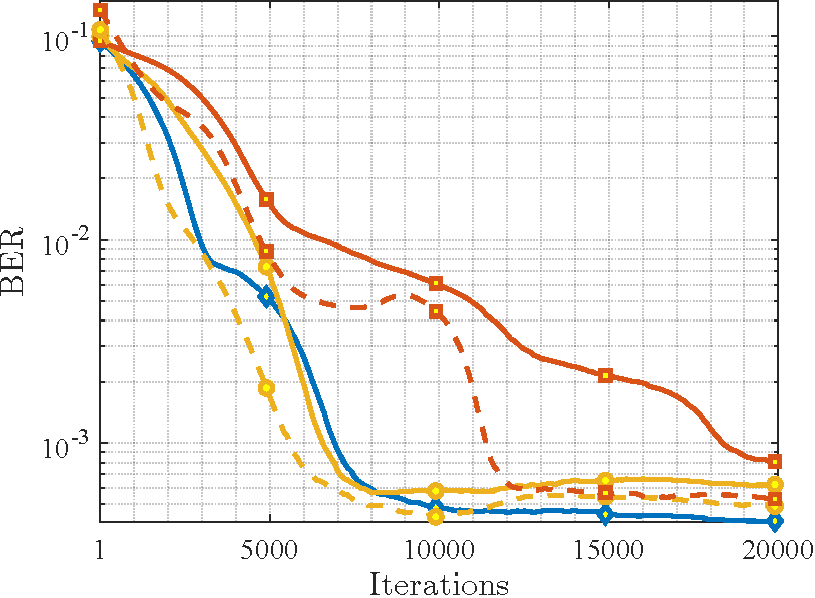
\includegraphics[width=\textwidth]{figures/BER_3.pdf}
%          \caption{BER}
%          \label{fig:ber_3}
%      \end{subfigure}
%      \hfill
%      \begin{subfigure}[b]{0.48\textwidth}
%          \centering
%          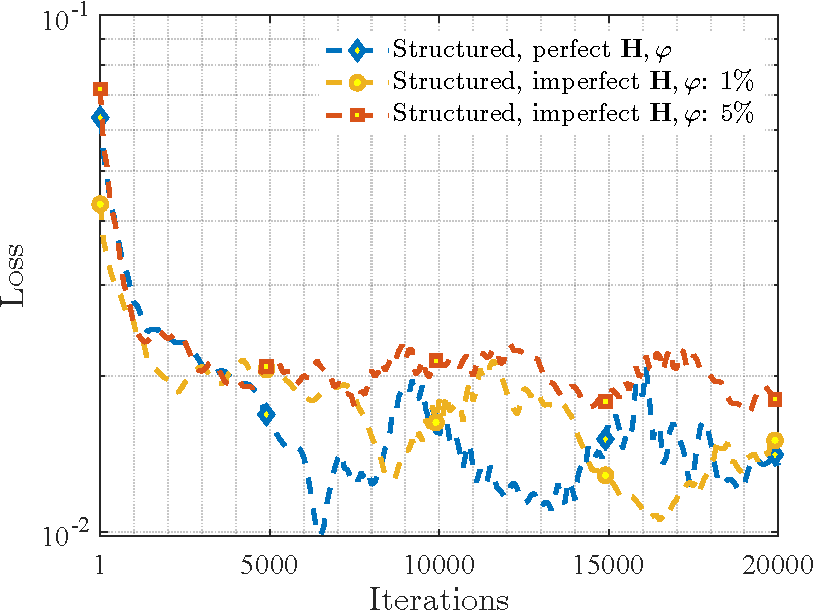
\includegraphics[width=\textwidth]{figures/Loss_3.pdf}
%          \caption{Mất mát}
%          \label{fig:loss_3}
%      \end{subfigure}
%      \hfill
%     \begin{subfigure}{\linewidth}
%         \centering
%         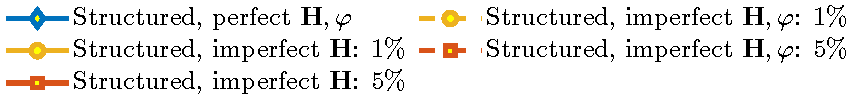
\includegraphics[width=.8\linewidth]{figures/lg_performance_31.pdf}
%     \end{subfigure}
%     \caption{Sự hội tụ của quá trình đào tạo các mạng ISDNN có cấu trúc với các sai số kênh truyền và thông tin bên lề đầu vào khác nhau.}
%     \label{fig:training_3}
% \end{figure}

% Trên hình~\ref{fig:training_3} là kết quả đào tạo của mạng ISDNN có cấu trúc khi các bộ dữ liệu huấn luyện có cả sai số trong $\mathbf{H}$ và ${\boldsymbol{\varphi}}$. Với việc cả hai ma trận trên đều có sai số sẽ hình thành sai số tích lũy cho các đầu vào như $\hat{\mathbf{s}}, \hat{\mathbf{x}}, \mathbf{D},~\ldots$ có thể gây khó khăn cho bộ nhận dạng. Trước hết trên hình~\ref{fig:loss_3} là đầu ra của hàm mất mát thu được trong suốt quá trình đào tạo. Tuy có thêm sai số đầu vào từ DoA, nhưng giá trị đầu ra của hàm mất mát lại cho thấy điều ngược lại, khi có thêm sai số này, mạng ISDNN hội tụ nhanh hơn cả trường hợp khi chỉ có sai số của kênh truyền $\mathbf{H}$. Đặc biệt, với trường hợp cả $\mathbf{H}$ và ${\boldsymbol{\varphi}}$ đều có sai số $5\%$, sau $12.000$ vòng đào tạo, giá trị hàm mất mát đã đạt được giá trị hội tụ và ổn định như trường hợp không có sai số. Tương tự với kết quả của BER trong quá trình đào tạo trên hình~\ref{fig:ber_3}, khi có thêm sai số của $\boldsymbol{\varphi}$, đường BER còn có độ lớn hơn trong trường hợp chỉ có sai số của ma trận kênh truyền.
% Chỉ sau $3.000$ vòng đào tạo, cả ba bộ dữ liệu đều cho ra giá trị hàm mất mát khoảng $2*10^{-2}$. Sau đó, trong trường hợp không có sai số và sai số $1$\% trong tập huấn luyện, giá trị của hàm mất mát vẫn tiếp tục đi xuống nhưng vẫn biến thiên, không hội tụ. Trong khi đó, trường hợp sai số $5$\% lại cho ra giá trị khá ổn định xung quanh khoảng $2*10^{-2}$. Với BER trên hình~\ref{fig:ber_3}, cả ba tập dữ liệu đều có thời điểm đạt được $\operatorname{BER} \approx 10^{-3}$ nhưng đều không giữ được giá trị này mà tiếp tục biến thiên không theo quy luật.

% Mạng ISDNN có cấu trúc được lưu tại vòng lặp cuối cùng của việc học và thử nghiệm với các giá trị SNR khác nhau như trên hình. 
Khi có sai số về ma trận $\boldsymbol{\varphi}$, đường BER đầu ra sẽ cho kết quả kém hơn một chút so với khi chỉ có sai số về $\mathbf{H}$ như trên hình~\ref{fig:isdnn_3}. Tuy nhiên, cũng như trong quá trình học, đường BER khi sai số của $\mathbf{H}$ và $\boldsymbol{\varphi}$ ở mức $5\%$ cho kết quả không ổn định. Tại $\operatorname{SNR}=15$~dB, BER của ISDNN còn tốt hơn trường hợp chỉ có sai số $1\%$ của bộ dữ liệu. Nguyên nhân có thể xuất phát từ việc gieo ngẫu nhiên những sai số trong bộ dữ liệu đầu vào, tạo nên ma trận $\hat{\boldsymbol{\beta}}$ tốt hơn ở giá trị SNR này. Trong trong hợp này, so sánh với hình~\ref{fig:isdnn_1}, kết quả mô hình đầu ra trong hai trường hợp có sai số từ $\mathbf{H}$ và thông tin bên lề của mạng ISDNN có cấu trúc là tương đương với mạng ISDNN không sử dụng cấu trúc chỉ có sai số về ma trận kênh truyền.
% \section{Kết luận chương}
\begin{figure}[H]
    \centering
    \begin{subfigure}{\linewidth}
        \centering
        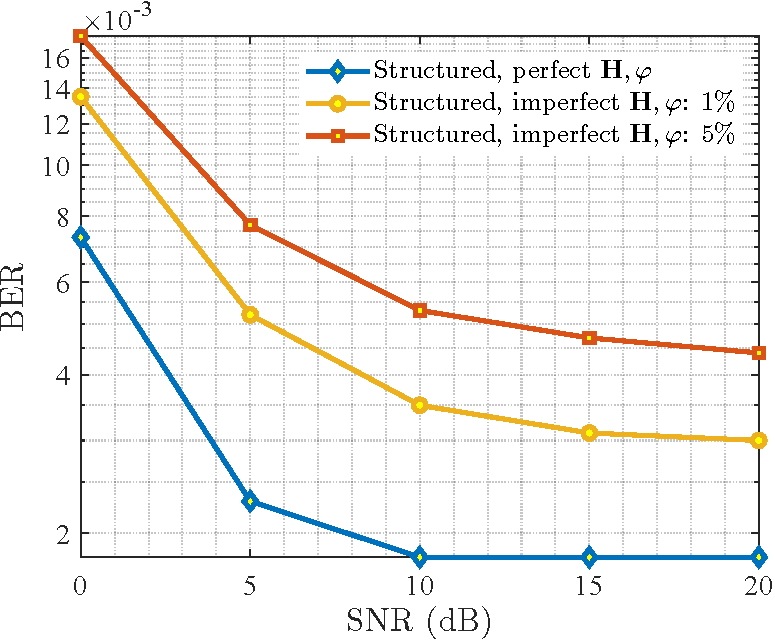
\includegraphics[width=.6\linewidth]{figures/performance_3.pdf}
    \end{subfigure}
    \hfill
    \begin{subfigure}{\linewidth}
        \centering
        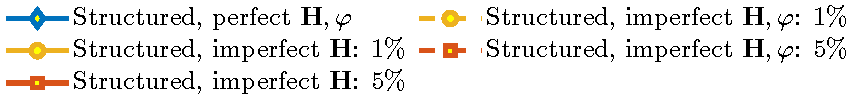
\includegraphics[width=.6\linewidth]{figures/lg_performance_31.pdf}
    \end{subfigure}
    \caption{Độ chính xác của mạng ISDNN có cấu trúc với các sai số kênh truyền và thông tin bên lề đầu vào khác nhau.}
    \label{fig:isdnn_3}
\end{figure}
% Trong chương này, tác giả đã trình bày khái quát về việc sử dụng DNN và mở rộng sâu cho việc nhận dạng kênh truyền. Tiếp đến, một kiến trúc mạng nơ-ron sâu tên DetNet đã được đề xuất trước đây được trình bày ngắn gọn. Từ một phương pháp nhận dạng không mù với độ phức tạp thấp ISD đã được công bố trước đó, kiến trúc ISDNN mới được đề xuất cho cả hai mô hình kênh truyền có cấu trúc và không sử dụng cấu trúc sử dụng phương pháp mở rộng sâu. Kết quả mô phỏng đã chỉ ra hiệu năng về độ chính xác và độ phức tạp của kiến trúc ISDNN được đề xuất. Trước hết, về độ chính xác, ISDNN cho kết quả vượt trội so với các thuật toán nhận dạng tuyến tính không mù như ZF, MMSE, và mạng nơ-ron sâu DetNet dù với số lượng lớp mạng ít hơn. Về độ phức tạp, so với các giải thuật tuyến tính, ISDNN cho độ lợi $\mathcal{O}(L)$ tương tự như DetNet. Hơn nữa, ISDNN chỉ cần $24$ tham số học cho $4$ lớp mạng khi so sánh với $105.416$ tham số của mạng DetNet cùng số lớp mạng. Từ hai khía cạnh trên, kết luận mạng ISDNN đã giải quyết cả hai vấn đề là độ phức tạp, và chính xác đã được đề ra ở phần Mở đầu. Kiến trúc ISDNN được đề xuất cho mô hình kênh truyền có cấu trúc cũng cho độ chính xác là tốt hơn so với ISDNN không sử dụng cấu trúc như đã chỉ ra trong chương~\ref{sec:CRB}.
% Ngoài ra, để xem xét khả năng ứng dụng vào thực tế, hiệu suất của ISDNN được xem xét nếu có sai số trong các bộ dữ liệu đầu vào, có thể xảy ra bởi sai số đo lượng. Các kết quả mô phỏng chỉ ra sự ảnh hưởng của tập dữ liệu huấn luyện đến kết quả đào tạo. Tuy nhiên, sai số cũng ở mức chấp nhận được và vẫn là tốt hơn nếu so sánh với các phương pháp đã kể trên. 
\newpage
\clearpage
\phantomsection

\addcontentsline{toc}{chapter}{KẾT LUẬN}
\chapter*{Kết luận}

Trong luận văn, tác giả tập trung giải quyết các thách thức về chi phí và độ phức tạp của các phương pháp nhận dạng trong các thế hệ mạng di động mới sử dụng mMIMO. Trước hết, các phương pháp mô hình kênh truyền trong mMIMO được khảo sát để chọn ra phương pháp phù hợp cho nghiên cứu trong luận văn. Tiếp đến,
một khảo sát về bốn phương pháp nhận dạng hệ thống viễn thông không dây được trình bày. Qua đó, chỉ ra được sự cần thiết của việc ứng dụng tri thức mới vào bài toán nhận dạng hệ thống thông qua hai hướng tiếp cận là bán mù và sử dụng học sâu. 
Từ đó, trong chương~\ref{sec:CRB}, tác giả xem xét sự ảnh hưởng của các cấu hình mảng ăng-ten khác nhau và giải thuật SB đến độ chính xác của việc ước lượng kênh truyền dựa trên CRB. Kết quả chỉ ra rằng việc mô hình kênh truyền có cấu trúc, sử dụng các mảng ăng-ten 3D như UCyA, hay phương pháp SB đều có thể giúp giảm sai số của việc ước lượng kênh truyền đi đáng kể. Ngoài ra việc sử dụng các mảng ăng-ten 3D sẽ giúp tiết kiệm diện tích lắp đặt cho các trạm cơ sở đi đáng kể khi so sánh với các cấu hình ULA truyền thống.
Trong chương~\ref{sec:ML}, hướng tiếp cận học sâu, sử dụng thêm thông tin bên lề về hướng sóng đến và cấu hình mảng ăng-ten, cũng được tác giả xem xét để nhận dạng kênh truyền cho hệ thống mMIMO. Cụ thể, một mạng ISDNN được đề xuất nhằm giảm thiểu độ phức tạp và chi phí so với thuật toán ISD gốc dựa trên bộ nhận dạng MMSE. Kiến trúc mạng nơ-ron sâu được đề xuất chỉ yêu cầu $24$ tham số học và $7$~KB cho mô hình được đào tạo với cấu hình gồm $4$ lớp mạng. Đây là số lượng rất nhỏ và hoàn toàn vượt trội khi so sánh với một mạng nơ-ron sâu khác cũng với cách tiếp cận tương tự là DetNet. Từ các kết quả mô phỏng, hiệu suất về thời gian đào tạo và độ chính xác của ISDNN cũng được kiểm chứng là vượt trội cả các phương pháp tuyến tính và mạng nơ-ron sâu DetNet.
Ngoài ra, tác giả cũng xem xét đến hiệu suất của mạng nếu dữ liệu đầu vào xuất hiện sai số trong việc đo lường. Kết quả thu được cho thấy sự ảnh hưởng rõ ràng của sai số từ dữ liệu huấn luyện đến mô hình. Tuy nhiên sau khi đào tạo, độ chính xác của mô hình được đề xuất vẫn giữ được dạng gốc và vẫn có phần vượt trội so với các phương pháp khác tương tự như khi không có sai số trong dữ liệu. 

Kết quả nghiên cứu của chương~\ref{sec:CRB} đã được công bố:
\begin{enumerate}
    \item[] \textbf{Do Hai Son} and Tran Thi Thuy Quynh (2023), ``Impact Analysis of Antenna Array Geometry on Performance of Semi-Blind Structured Channel Estimation for massive MIMO-OFDM systems,'' in \textit{IEEE Statistical Signal Processing Workshop (SSP)}, Hanoi, Vietnam, July. [accepted]
\end{enumerate}

\def\baselinestretch{1}
\vspace{-2cm}
% \clearpage
% \phantomsection
% \addcontentsline{toc}{chapter}{TÀI LIỆU THAM KHẢO}
% \renewcommand{\bibname}{Tài liệu tham khảo}
% \bibliographystyle{./footage/agsm_uet.bst}
% \bibliography{library.bib}

\end{document}